%%%%%%%%%%%%%%%%%%%%%%%%%%%%%%%%%%%%%%%%%%%%%%%%%%%%%%%%%%%%%%%%%%%%%
% Overleaf (WriteLaTeX) Example: Molecular Chemistry Presentation
%
% Source: http://www.overleaf.com
%
% In these slides we show how Overleaf can be used with standard 
% chemistry packages to easily create professional presentations.
% 
% Feel free to distribute this example, but please keep the referral
% to overleaf.com
% 
%%%%%%%%%%%%%%%%%%%%%%%%%%%%%%%%%%%%%%%%%%%%%%%%%%%%%%%%%%%%%%%%%%%%%%

\documentclass[dvipsnames]{beamer}

\mode<presentation>
{
  \usetheme{Madrid}       % or try default, Darmstadt, Warsaw, ...
  \usecolortheme{default} % or try albatross, beaver, crane, ...
  \usefonttheme{default}    % or try default, structurebold, ...
  \setbeamertemplate{navigation symbols}{}
  \setbeamertemplate{caption}[numbered]
} 

\usepackage[english]{babel}
\usepackage[utf8x]{inputenc}
\usepackage{graphicx}
\usepackage{hyperref}
  \hypersetup{colorlinks=true}
  \hypersetup{urlcolor=blue}
  \hypersetup{linkcolor = .}
\usepackage{xcolor}
\usepackage{siunitx}
  \sisetup{separate-uncertainty = true}
\usepackage{physics}
\usepackage[font=small,labelfont=bf]{caption}
\usepackage{subcaption}
\usepackage[en-GB]{datetime2}
\usepackage{overpic}
\usepackage{feynmp}
\DeclareGraphicsRule{*}{mps}{*}{}
\usepackage{scalerel}
\newcommand{\mylbrace}[2]{\vspace{#2pt}\hspace{6pt}\scaleleftright[\dimexpr5pt+#1\dimexpr0.06pt]{\lbrace}{\rule[\dimexpr2pt-#1\dimexpr0.5pt]{-4pt}{#1pt}}{.}}
\newcommand{\myrbrace}[2]{\vspace{#2pt}\scaleleftright[\dimexpr5pt+#1\dimexpr0.06pt]{.}{\rule[\dimexpr2pt-#1\dimexpr0.5pt]{-4pt}{#1pt}}{\rbrace}\hspace{6pt}}

% Trim in percent
\usepackage{adjustbox}

% No "Figure" prefix
\setbeamertemplate{caption}{\raggedright\insertcaption\par}

% Nice decay amplitude diagrams
\usepackage{amsmath,amssymb,tikz-cd}

% Strike out text
\usepackage[normalem]{ulem}

% Vector arrows
\usepackage[pdftex]{pict2e}

% Tikz with shapes
\usepackage{tikz}
\usetikzlibrary{positioning,shapes}

% Here's where the presentation starts, with the info for the title slide
\title[CERN LHC seminar]{The angle $\gamma$ of the Cabibbo-Kobayashi-Maskawa ansatz: a journey towards precision at LHCb}

\author[Martin Tat]{Martin Tat, on behalf of the LHCb collaboration}
\institute[University of Oxford]{\normalsize University of Oxford\\ \vspace{0.3cm}\normalsize CERN LHC seminar}
\date{25th July 2023}

\titlegraphic{
\includegraphics[height = 2.5cm]{lhcb.jpg}\hspace{2.5cm}~%
              
\includegraphics[height = 2.5cm]{OxfordLogo.pdf}}

\begin{document}

\begin{frame}
  \titlepage
\end{frame}

% These three lines create an automatically generated table of contents.
% \begin{frame}{Outline}
%   \tableofcontents
% \end{frame}

\section{Introduction to \texorpdfstring{$C\!P$}{CP} violation}
\begin{frame}{Introduction to $C\!P$ violation}
  \begin{center}
    {\huge Introduction to $C\!P$ violation} \\~\\
    {\large What is $\gamma$ and why measure it?}
  \end{center}
\end{frame}

\begin{frame}{Big Bang and matter-antimatter asymmetry}
  \begin{figure}
    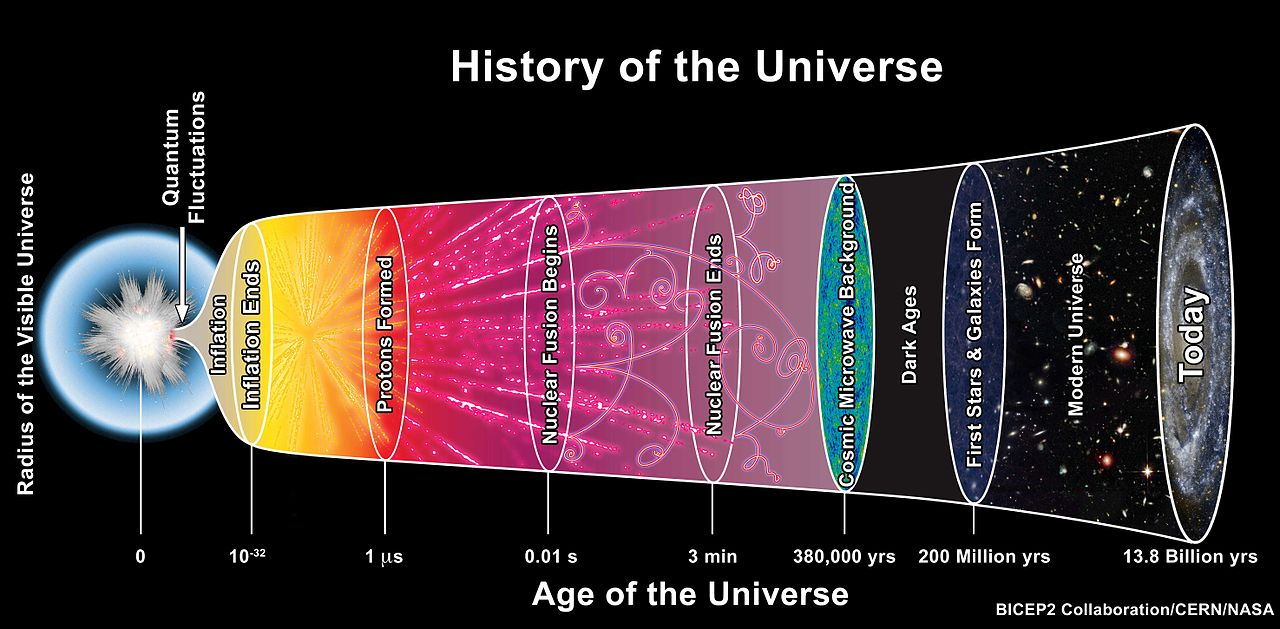
\includegraphics[height=5.5cm]{Plots/BigBangHistory.jpg}
  \end{figure}
  \begin{center}
    \Large Where is the antimatter in the universe?\phantom{yq}
  \end{center}
\end{frame}

\begin{frame}{Big Bang and matter-antimatter asymmetry}
  \begin{figure}
    \adjustbox{trim={0} {0} {0.838\width} {0},clip=true}{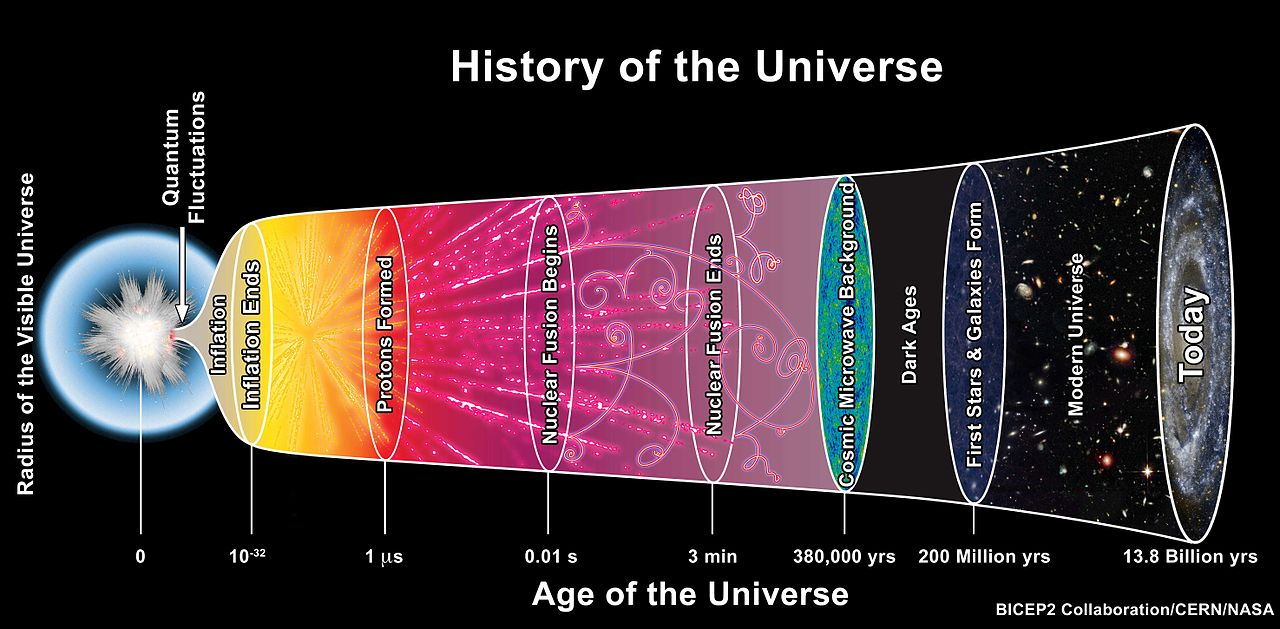
\includegraphics[height=5.5cm]{Plots/BigBangHistory.jpg}}%
    \adjustbox{trim={0.162\width} {0} {0} {0},clip=true}{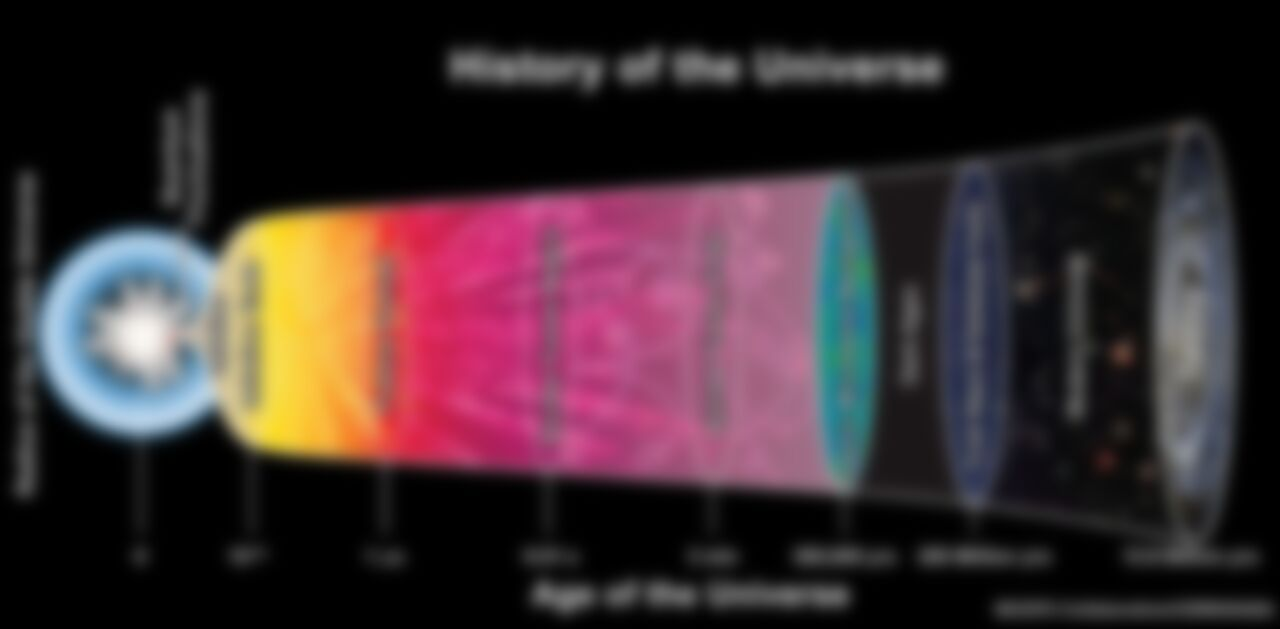
\includegraphics[height=5.5cm]{Plots/BigBangHistory_blur.jpg}}
  \end{figure}
  \begin{center}
    \Large Initially equal amounts of matter and antimatter...
  \end{center}
\end{frame}

\begin{frame}{Big Bang and matter-antimatter asymmetry}
  \begin{figure}
    \adjustbox{trim={0} {0} {0.18\width} {0},clip=true}{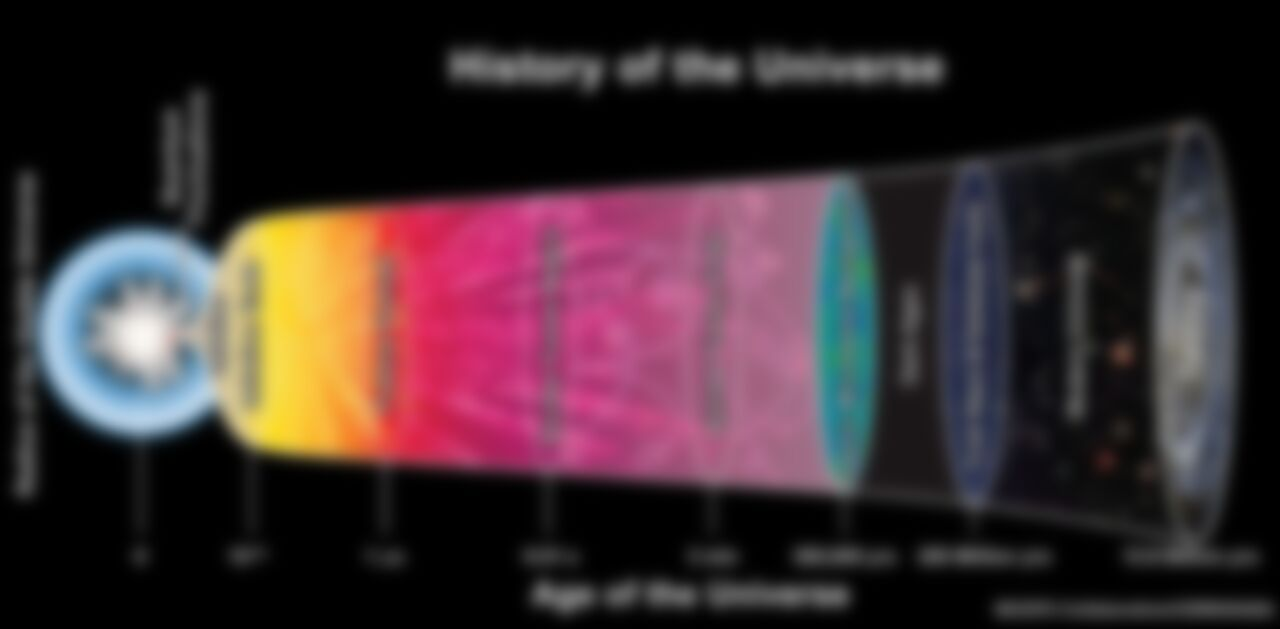
\includegraphics[height=5.5cm]{Plots/BigBangHistory_blur.jpg}}%
    \adjustbox{trim={0.82\width} {0} {0} {0},clip=true}{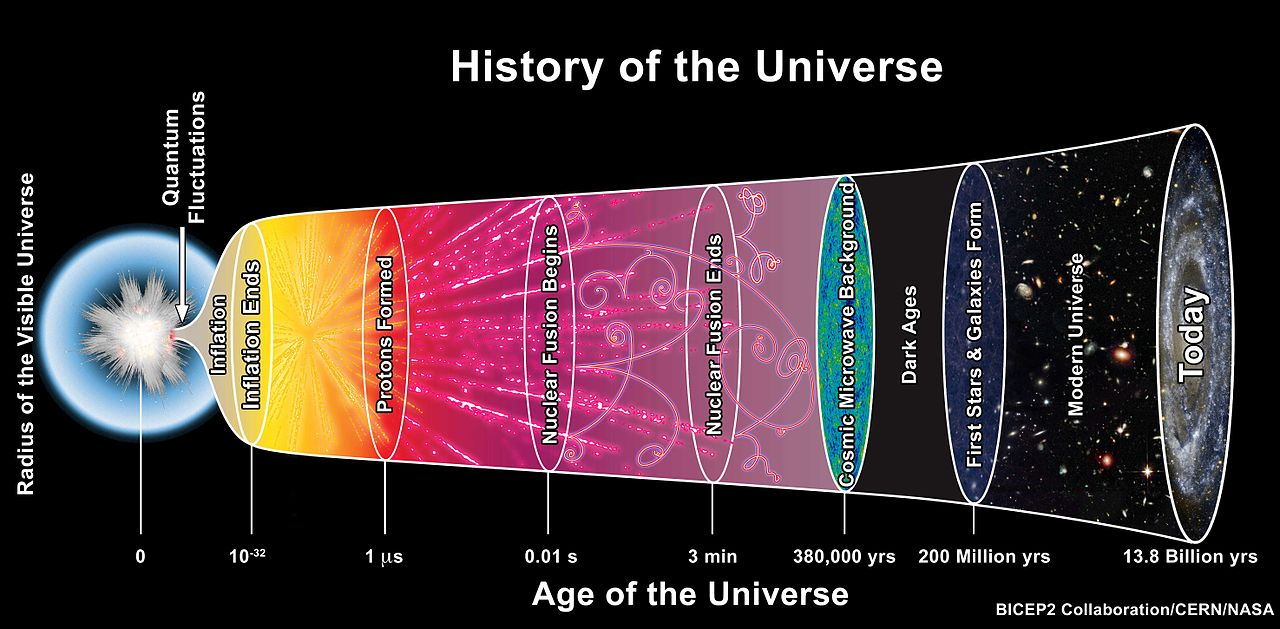
\includegraphics[height=5.5cm]{Plots/BigBangHistory.jpg}}
  \end{figure}
  \begin{center}
    \Large ... but today we only see matter!
  \end{center}
\end{frame}

\begin{frame}{Big Bang and matter-antimatter asymmetry}
  \begin{figure}
    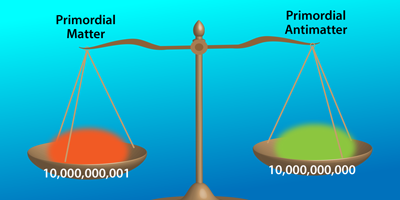
\includegraphics[width=0.8\textwidth,trim={0.9cm 0 0.9cm 0},clip=true]{Plots/PrimordialAntimatter.png}
    \caption*{\tiny APS/Alan Stonebraker}
  \end{figure}
  \vspace{-0.5cm}
  \begin{center}
    \Large The difference is very small...
  \end{center}
\end{frame}

\begin{frame}{Big Bang and matter-antimatter asymmetry}
  \begin{figure}
    
\includegraphics[width=0.45\textwidth]{Plots/MatterAntimatterBigAsymmetry.png}
    \caption*{\tiny Quantum Diaries: ``Why B physics? Why not A Physics?''}
  \end{figure}
  \vspace{-0.5cm}
  \begin{center}
    \Large ... but the effects we observe today are obviously huge! How can we explain this?
  \end{center}
\end{frame}

\begin{frame}{Big Bang and matter-antimatter asymmetry}
  \begin{columns}
    \begin{column}{0.4\textwidth}
      \begin{figure}
        
\includegraphics[width=1.0\textwidth]{Plots/NobelPeacePrize1975.png}
      \end{figure}
    \end{column}
    \begin{column}{0.6\textwidth}
      In 1967, Andrei Sakharov proposed three conditions for baryogenesis:
      \begin{itemize}
        \setlength\itemsep{1.0em}
        \item{Baryon number violation}
        \item{\underline{C and CP violation}}
        \item{Interactions out of thermal equilibrium}
      \end{itemize}
    \end{column}
  \end{columns}
  \vspace{0.5cm}
  \begin{center}
    \large Therefore, to understand matter-antimatter asymmetry, we must understand \underline{CP violation}
  \end{center}
\end{frame}

\begin{frame}{$C\!P$ violation}
  \begin{columns}
    \begin{column}{0.4\textwidth}
      \begin{figure}
        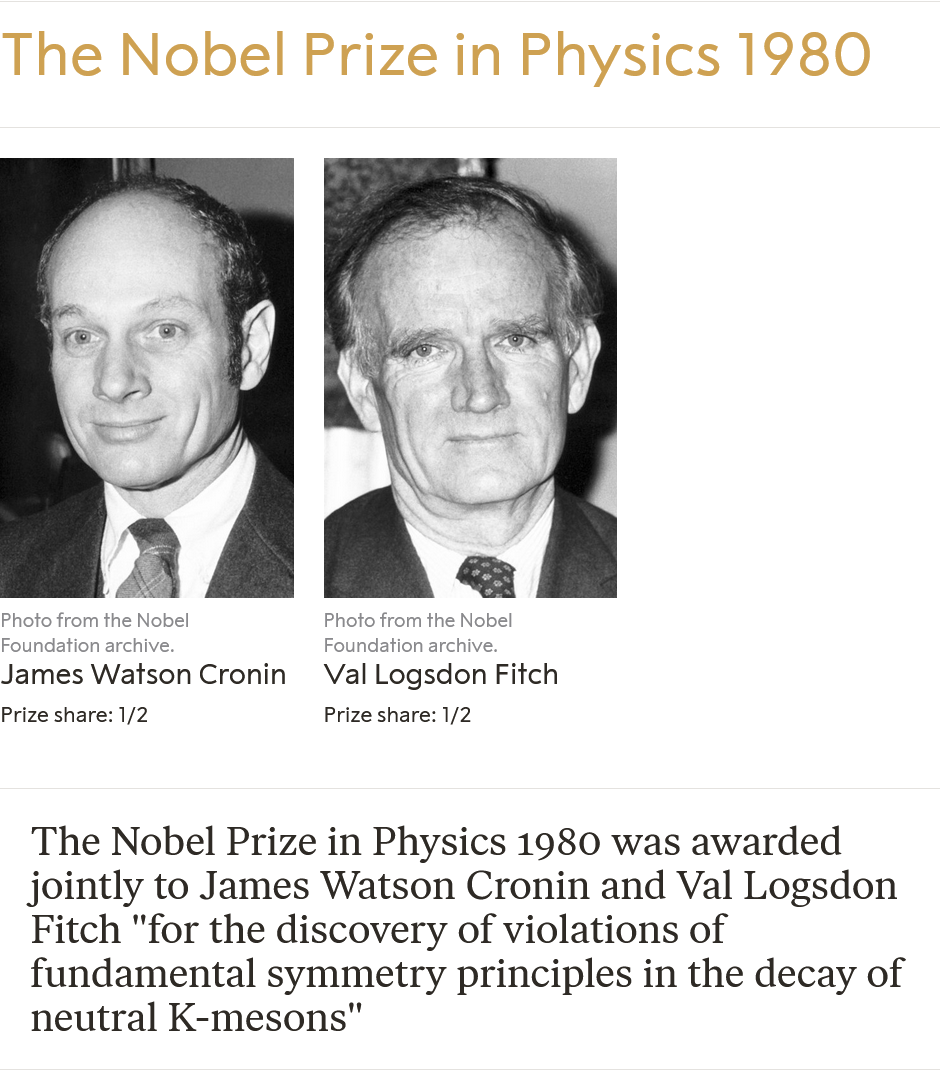
\includegraphics[width=1.0\textwidth]{Plots/NobelPrizePhysics1980.png}
      \end{figure}
    \end{column}
    \begin{column}{0.6\textwidth}
      \begin{itemize}
        \setlength\itemsep{1.0em}
        \item{$C\!P$ violation discovery in 1964}
        \item{Phys. Rev. Lett. \textbf{13}, 138}
        \item{Observed $K_L^0\to\pi^+\pi^-$}
        \item{Since, $C\!P$ violation has also been observed in the $B$, $B_s$ and $D$ systems}
      \end{itemize}
    \end{column}
  \end{columns}
  \vspace{0.5cm}
  \begin{center}
    \large Unfortunately, CPV in SM is too small to explain baryogenesis...\\... perhaps there are new physics effects?
  \end{center}
\end{frame}

\begin{frame}{The CKM matrix and the Unitary Triangle}
  \begin{center}
    In SM, the charged current $W^\pm$ interactions couple (left-handed) up- and down-type quarks, given by
  \end{center}
  \begin{equation*}
    \frac{-g}{\sqrt{2}}
    \begin{bmatrix}
      \bar{u_L} & \bar{c_L} & \bar{t_L}
    \end{bmatrix}
    \gamma^\mu W_\mu V_{\rm CKM}
    \begin{bmatrix}
      d_L \\
      s_L \\
      b_L
    \end{bmatrix}
     + {\rm h.c.}
  \end{equation*}
  \begin{figure}[H]
    \centering
    \vspace{0.3cm}
    \begin{subfigure}{0.5\textwidth}
      \centering
      \begin{fmffile}{fgraph/fgraph_W1}
        \setlength{\unitlength}{0.4cm}
        \begin{fmfgraph*}(6,6)
          \fmfstraight
          \fmfleft{i1}
          \fmfright{o1,o2}
          \fmflabel{$t$}{i1}
          \fmflabel{$b$}{o1}
          \fmflabel{$W^+$}{o2}
          \fmf{fermion}{i1,v}
          \fmf{fermion}{v,o1}
          \fmf{boson}{v,o2}
        \end{fmfgraph*}
      \end{fmffile}
      \vspace{0.5cm}
      \caption{$t\to bW^+$}
    \end{subfigure}%
    \begin{subfigure}{0.5\textwidth}
      \centering
      \begin{fmffile}{fgraph/fgraph_W2}
        \setlength{\unitlength}{0.4cm}
        \begin{fmfgraph*}(6,6)
          \fmfstraight
          \fmfleft{i1}
          \fmfright{o1,o2}
          \fmflabel{$b$}{i1}
          \fmflabel{$c$}{o1}
          \fmflabel{$W^-$}{o2}
          \fmf{fermion}{i1,v}
          \fmf{fermion}{v,o1}
          \fmf{boson}{v,o2}
        \end{fmfgraph*}
      \end{fmffile}
      \vspace{0.5cm}
      \caption{$b\to cW^-$}
    \end{subfigure}
  \end{figure}
\end{frame}

\begin{frame}{The CKM matrix and the Unitary Triangle}
  \begin{center}
    The Cabibbo-Kobayashi-Maskawa matrix $V_{\rm CKM}$ has a single complex phase that is responsible for all CPV in SM
  \end{center}
  \begin{equation*}
    \begin{bmatrix}
      V_{ud} & V_{us} & V_{ub} \\
      V_{cd} & V_{cs} & V_{cb} \\
      V_{td} & V_{ts} & V_{tb}
    \end{bmatrix} = 
    \setlength{\arraycolsep}{0pt}
    \begin{bmatrix}
      1 - \lambda^2/2              & \lambda         & \colorbox{Cerulean!30}{$A\lambda^3(\rho - i\eta)$} \\
      -\lambda                     & 1 - \lambda^2/2 & A\lambda^2 \\
      \colorbox{Cerulean!30}{$A\lambda^3(1 - \rho - i\eta)$} & -A\lambda^2     & 1 \\
    \end{bmatrix} + \mathcal{O}(\lambda^4)
  \end{equation*}
  \vspace{0.53cm}
  \begin{center}
    In SM, with only 3 generations of quarks, $V_{\rm CKM}$ must be unitary\\
    This gives us 9 constraints, one of which is:
  \end{center}
  \vspace{0.5cm}
  \begin{equation*}
    V^{\phantom{*}}_{ud}\colorbox{Cerulean!30}{$V^*_{ub}$} + V^{\phantom{*}}_{cd}V^*_{cb} + \colorbox{Cerulean!30}{$V^{\phantom{*}}_{td}$}V^*_{tb} = 0
  \end{equation*}
  \vspace{0.85cm}
\end{frame}

\begin{frame}{The CKM matrix and the Unitary Triangle}
  \begin{center}
    The Cabibbo-Kobayashi-Maskawa matrix $V_{\rm CKM}$ has a single complex phase that is responsible for all CPV in SM
  \end{center}
  \begin{equation*}
    \begin{bmatrix}
      V_{ud} & V_{us} & V_{ub} \\
      V_{cd} & V_{cs} & V_{cb} \\
      V_{td} & V_{ts} & V_{tb}
    \end{bmatrix} = 
    \setlength{\arraycolsep}{0pt}
    \begin{bmatrix}
      1 - \lambda^2/2              & \lambda         & \colorbox{Cerulean!30}{$A\lambda^3(\rho - i\eta)$} \\
      -\lambda                     & 1 - \lambda^2/2 & A\lambda^2 \\
      \colorbox{Cerulean!30}{$A\lambda^3(1 - \rho - i\eta)$} & -A\lambda^2     & 1 \\
    \end{bmatrix} + \mathcal{O}(\lambda^4)
  \end{equation*}
  \begin{figure}
    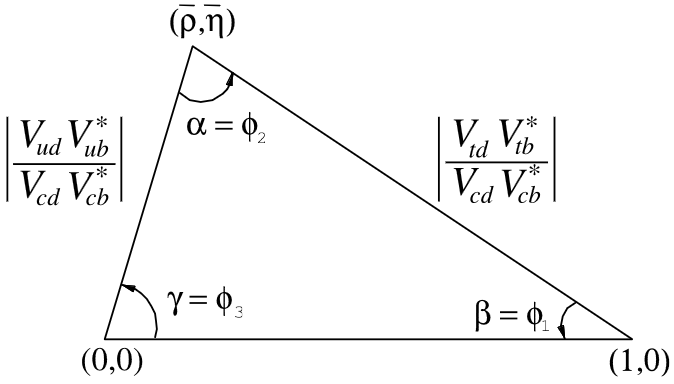
\includegraphics[width = 0.50\textwidth]{Plots/PDG_UnitaryTriangle.png}
    \vspace{-0.3cm}
    \caption*{\tiny R. L. Workman \textit{et al.} (Particle Data Group), Prog. Theor. Exp. Phys. 2022, 083C01 (2022)}
  \end{figure}
\end{frame}

\begin{frame}{The CKM matrix and the Unitary Triangle}
  \begin{columns}
    \begin{column}{0.4\textwidth}
      \begin{figure}
        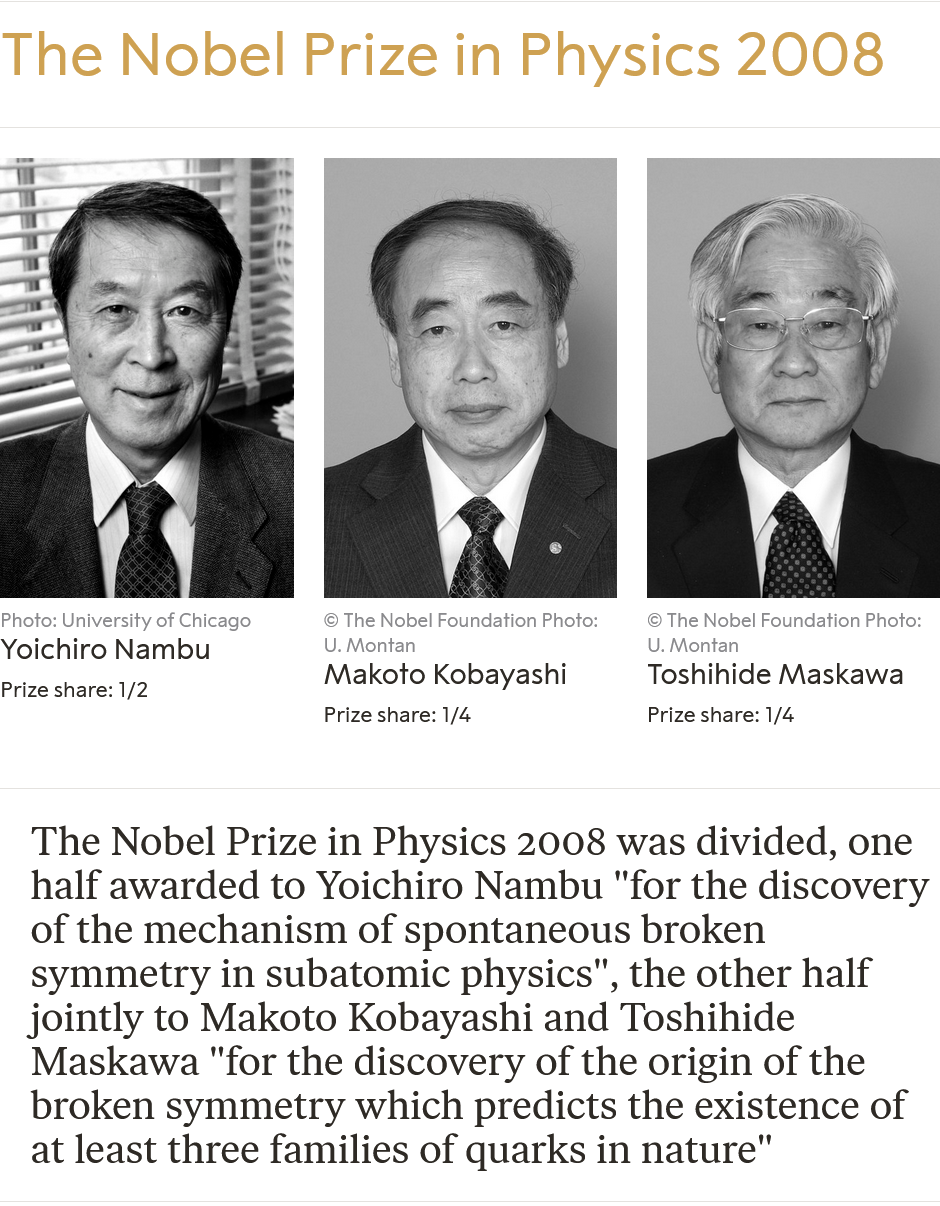
\includegraphics[width=1.0\textwidth]{Plots/NobelPrizePhysics2008.png}
      \end{figure}
    \end{column}
    \begin{column}{0.6\textwidth}
      \begin{itemize}
        \setlength\itemsep{1.0em}
        \item{Kobayashi and Maskawa extended Cabibbo's $2\times2$ rotation matrix}
        \item{The additional complex phase in $V_{\rm CKM}$ matrix explains CPV in SM}
        \item{This also predicted the third generation of quarks, which were discovered later}
      \end{itemize}
    \end{column}
  \end{columns}
  \begin{center}
    \large We must verify if $V_{\rm CKM}$ is unitary, and gain a deeper understanding of quark interactions
  \end{center}
\end{frame}

\begin{frame}{The CKM matrix and the Unitary Triangle}
  \begin{columns}
    \begin{column}{0.4\textwidth}
      \begin{figure}
        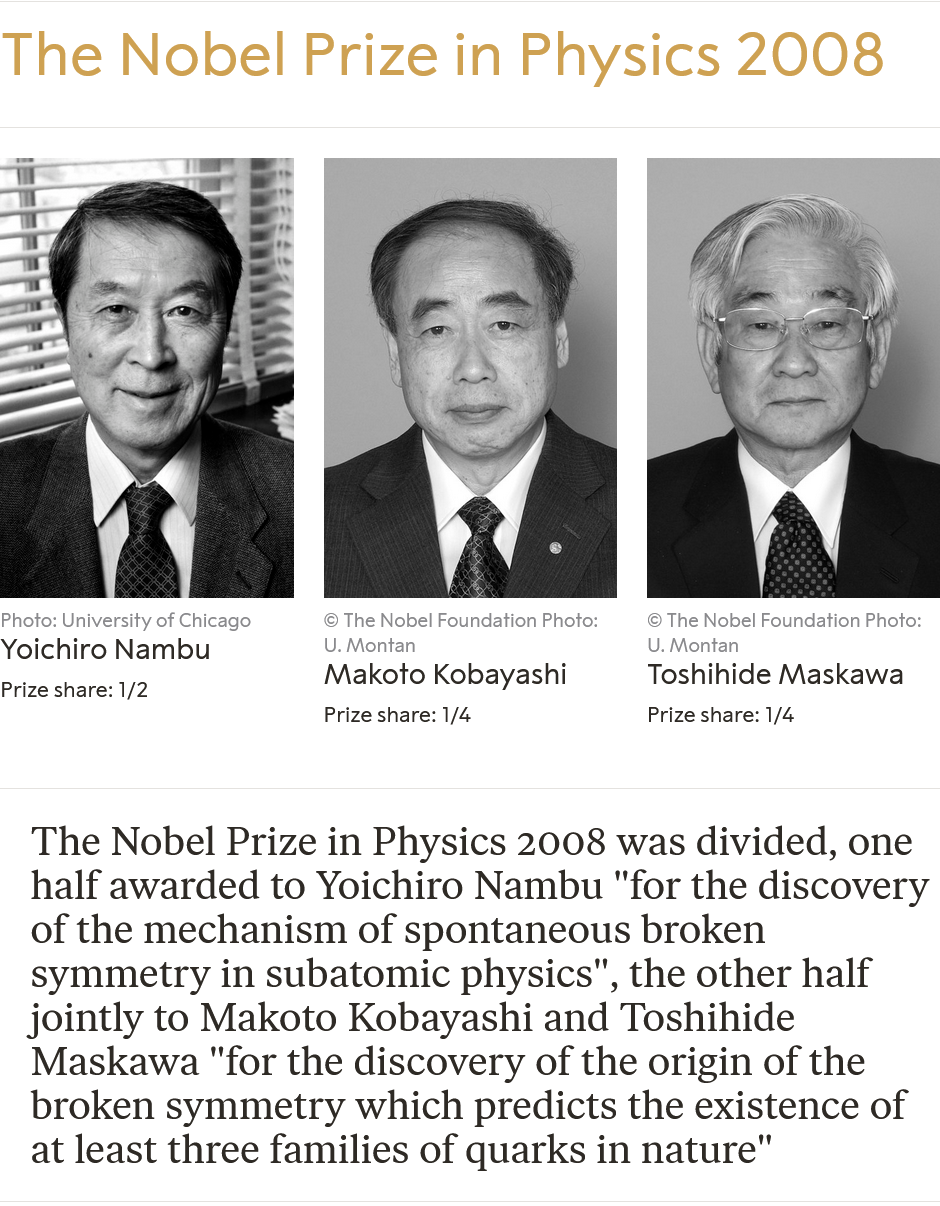
\includegraphics[width=1.0\textwidth]{Plots/NobelPrizePhysics2008.png}
      \end{figure}
    \end{column}
    \begin{column}{0.6\textwidth}
      \begin{itemize}
        \setlength\itemsep{1.0em}
        \item{Kobayashi and Maskawa extended Cabibbo's $2\times2$ rotation matrix}
        \item{The additional complex phase in $V_{\rm CKM}$ matrix explains CPV in SM}
        \item{This also predicted the third generation of quarks, which were discovered later}
      \end{itemize}
    \end{column}
  \end{columns}
  \begin{center}
    \large Precise knowledge of quark interactions will help us search for new physics with CPV, which may not have the same CKM structure
  \end{center}
\end{frame}

\begin{frame}{The CKM matrix and the Unitary Triangle}
  \begin{center}
    Before Belle and BaBar, the Unitary Triangle was poorly constrained
  \end{center}
  \vspace{-0.2cm}
  \begin{figure}
    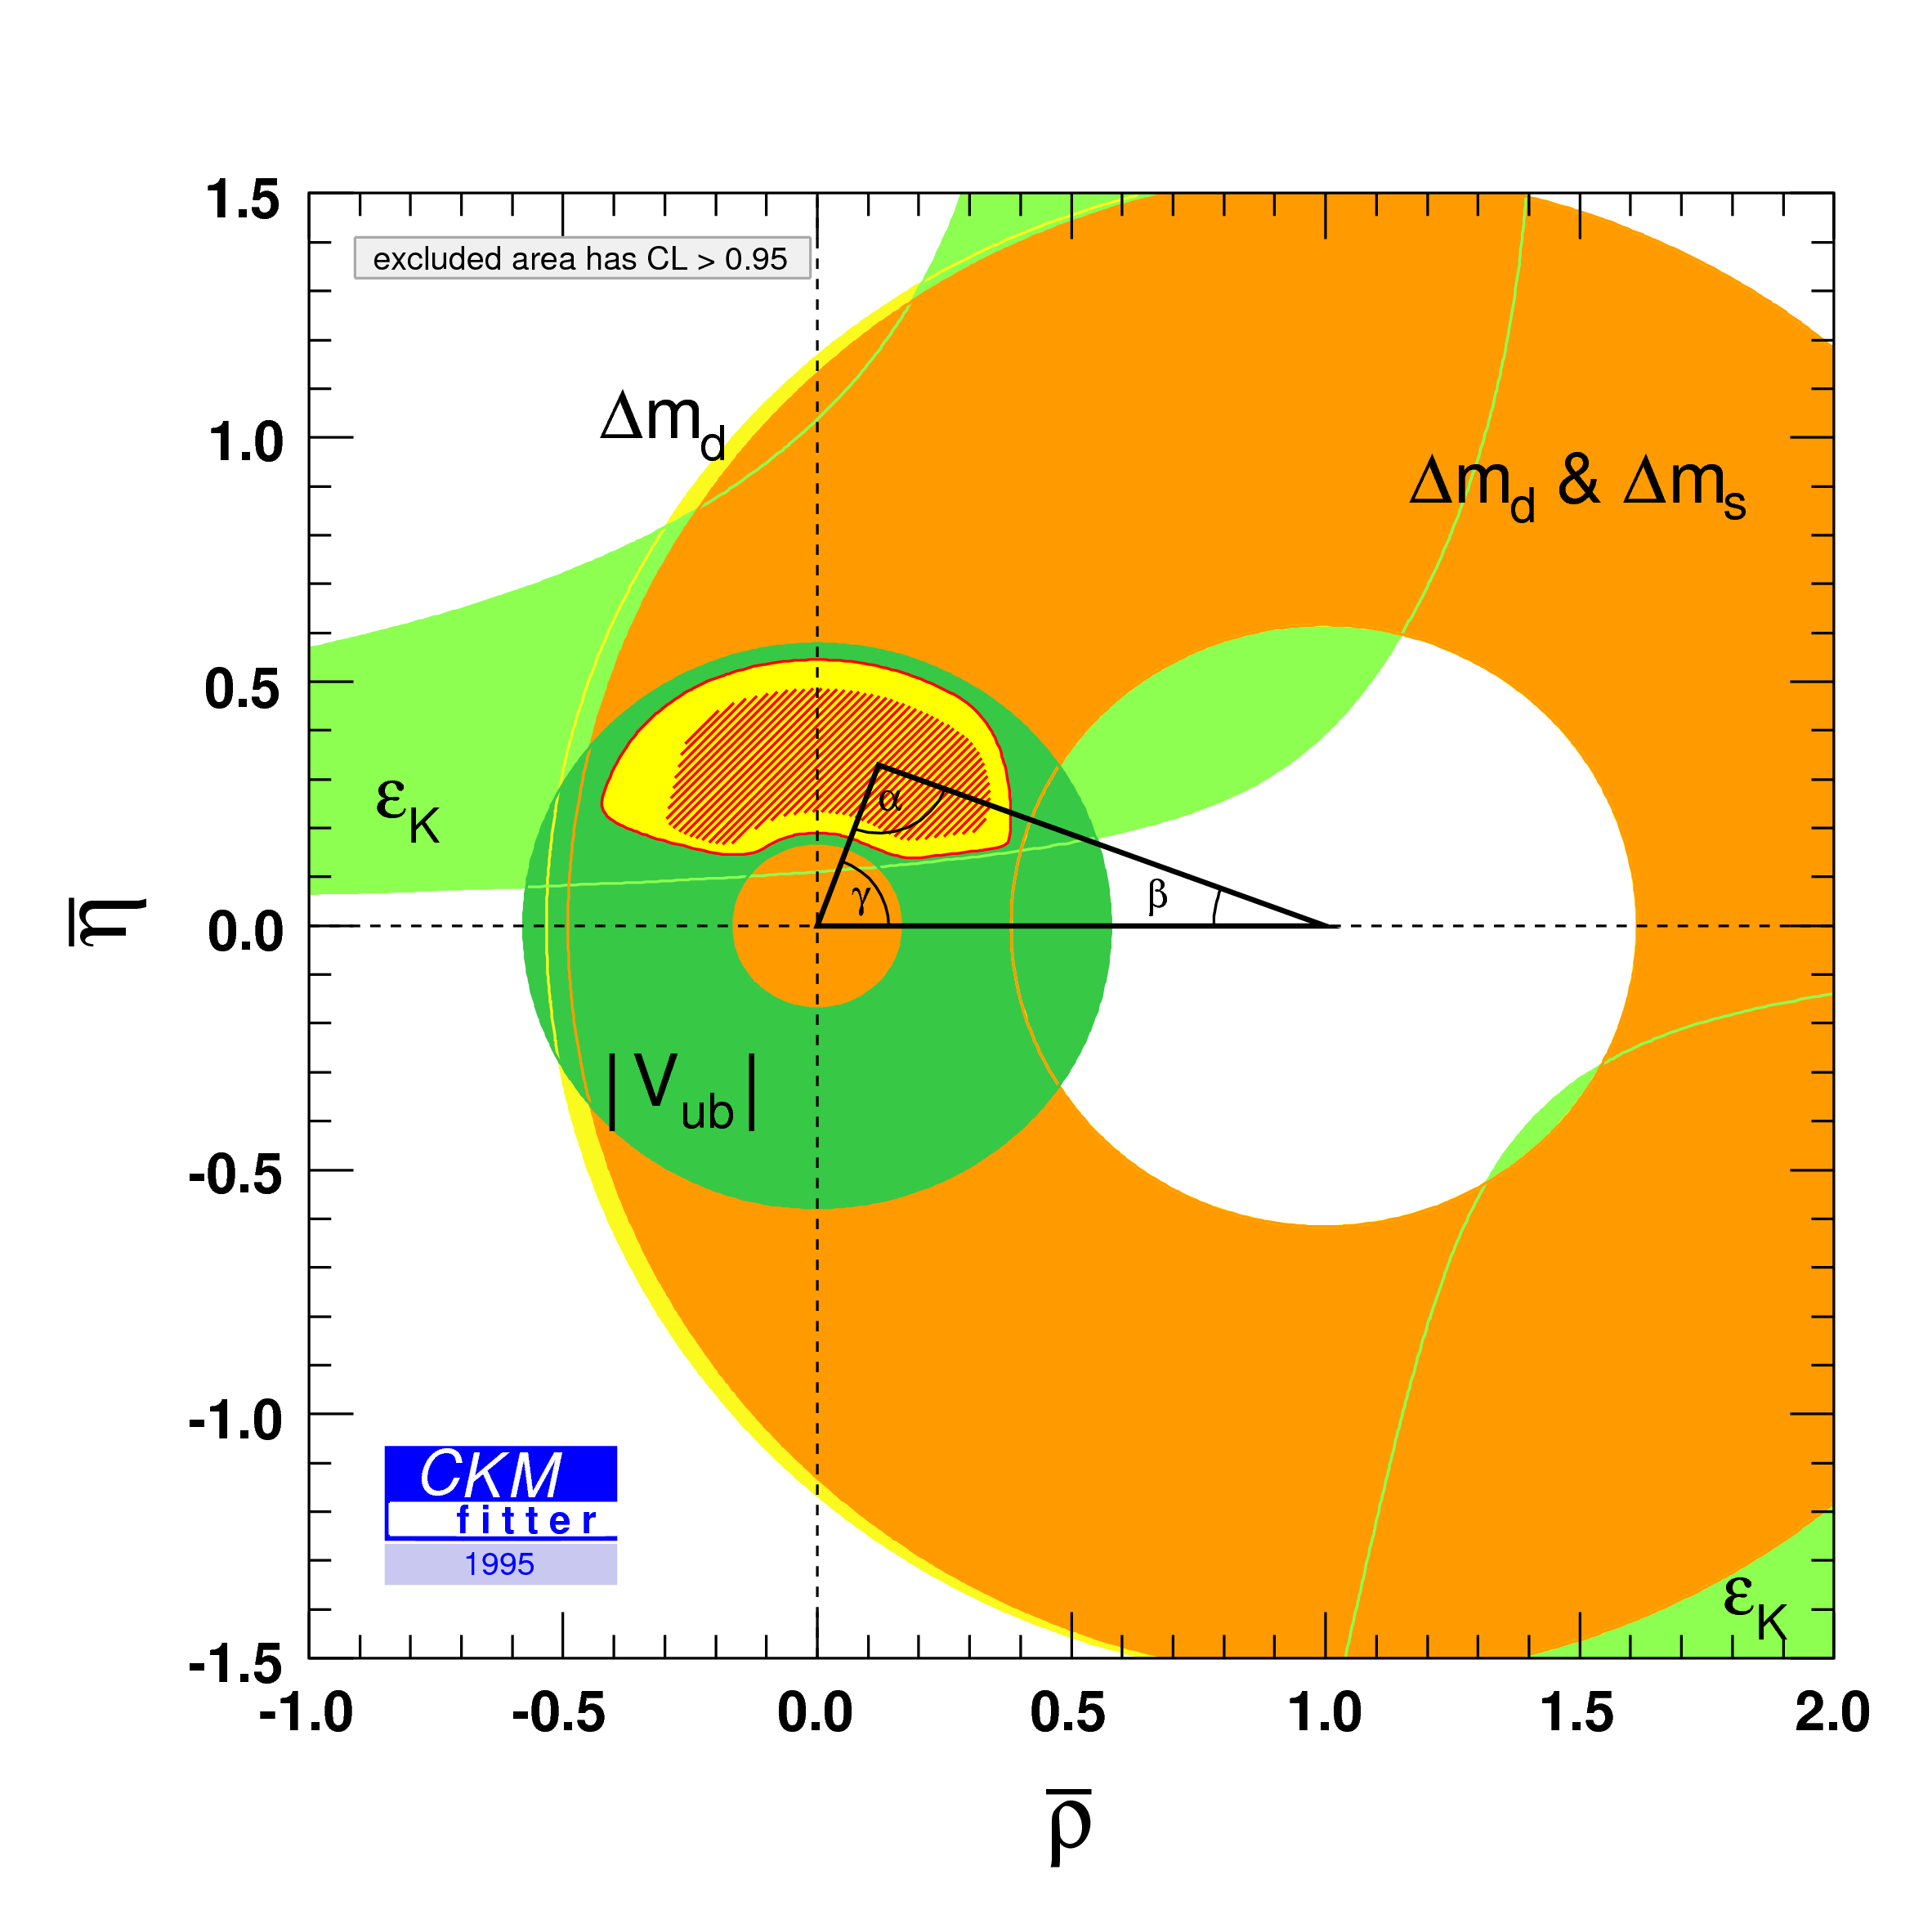
\includegraphics[width = 0.50\textwidth]{Plots/CKM_global_1995.png}
    \vspace{-0.3cm}
    \caption*{\centering\tiny CKMfitter Group (J. Charles et al.), Eur. Phys. J. C41, 1-131 (2005), updated results and plots available at: \href{http://ckmfitter.in2p3.fr}{http://ckmfitter.in2p3.fr}}
  \end{figure}
\end{frame}

\begin{frame}{The CKM matrix and the Unitary Triangle}
  \begin{center}
    Huge progess by b-factories, but $\gamma$ is the least precisely measured angle...
  \end{center}
  \vspace{-0.2cm}
  \begin{figure}
    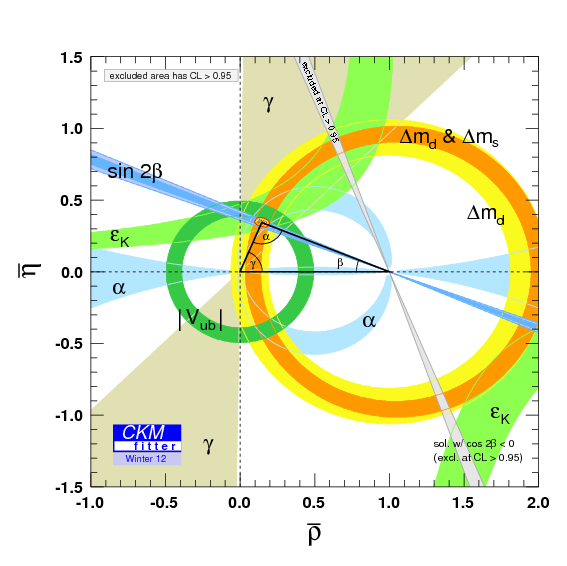
\includegraphics[width = 0.50\textwidth]{Plots/CKM_global_2012.png}
    \vspace{-0.3cm}
    \caption*{\centering\tiny CKMfitter Group (J. Charles et al.), Eur. Phys. J. C41, 1-131 (2005), updated results and plots available at: \href{http://ckmfitter.in2p3.fr}{http://ckmfitter.in2p3.fr}}
  \end{figure}
\end{frame}

\begin{frame}{The CKM matrix and the Unitary Triangle}
  \begin{center}
    ... but with LHCb, this is no longer the case!
  \end{center}
  \vspace{-0.2cm}
  \begin{figure}
    \begin{overpic}[percent,width=0.50\textwidth]{Plots/CKM_global_2021.png}
    \end{overpic}
    \vspace{-0.3cm}
    \caption*{\centering\tiny CKMfitter Group (J. Charles et al.), Eur. Phys. J. C41, 1-131 (2005), updated results and plots available at: \href{http://ckmfitter.in2p3.fr}{http://ckmfitter.in2p3.fr}}
  \end{figure}
\end{frame}

\begin{frame}{The CKM matrix and the Unitary Triangle}
  \begin{center}
    ... but with LHCb, this is no longer the case!
  \end{center}
  \vspace{-0.2cm}
  \begin{figure}
    \begin{overpic}[percent,width=0.50\textwidth]{Plots/CKM_global_2021.png}
      \put(0,7){\vector(1.0,1.35){50}}
      \put(0,7){\vector(1.0,0.8){35}}
      \put(-50,2){Direct $\gamma$ measurements}
    \end{overpic}
    \vspace{-0.3cm}
    \caption*{\centering\tiny CKMfitter Group (J. Charles et al.), Eur. Phys. J. C41, 1-131 (2005), updated results and plots available at: \href{http://ckmfitter.in2p3.fr}{http://ckmfitter.in2p3.fr}}
  \end{figure}
\end{frame}

\begin{frame}{The CKM matrix and the Unitary Triangle}
  \begin{center}
    ... but with LHCb, this is no longer the case!
  \end{center}
  \vspace{-0.2cm}
  \begin{figure}
    \begin{overpic}[percent,width=0.50\textwidth]{Plots/CKM_global_2021.png}
      \put(98,71){\vector(-1.0,-0.2){50}}
      \put(100,70){Global CKM fit}
    \end{overpic}
    \vspace{-0.3cm}
    \caption*{\centering\tiny CKMfitter Group (J. Charles et al.), Eur. Phys. J. C41, 1-131 (2005), updated results and plots available at: \href{http://ckmfitter.in2p3.fr}{http://ckmfitter.in2p3.fr}}
  \end{figure}
\end{frame}

\begin{frame}{The CKM matrix and the Unitary Triangle}
  \begin{center}
    Loop level measurements of $\gamma$ are dominated by $\sin(2\beta)$ and $B^0$/$B^0_s$ mixing
  \end{center}
  \vspace{-0.2cm}
  \begin{figure}
    \begin{overpic}[percent,width=0.50\textwidth]{Plots/CKM_global_2021.png}
      \put(98,71){\vector(-1.0,-0.2){50}}
      \put(100,70){Global CKM fit}
      \put(88,100){\vector(-1.0,-0.5){58}}
      \put(120,100){\vector(-1.0,-0.5){45}}
    \end{overpic}
    \vspace{-0.3cm}
    \caption*{\centering\tiny CKMfitter Group (J. Charles et al.), Eur. Phys. J. C41, 1-131 (2005), updated results and plots available at: \href{http://ckmfitter.in2p3.fr}{http://ckmfitter.in2p3.fr}}
  \end{figure}
\end{frame}

\begin{frame}{The CKM matrix and the Unitary Triangle}
  \begin{center}
    \Large LHC seminar by P. Li and V. Jevtic on 13th June 2023:\\
    \Large Single most precise measurement of $\sin(2\beta)$
  \end{center}
  \vspace{-0.3cm}
  \begin{figure}
    \centering
    \begin{subfigure}{0.55\textwidth}
      \begin{overpic}[width = 1.0\textwidth]{Plots/asym_sin2beta.pdf}
        \put(16.5,16.5){\tiny Preliminary}
      \end{overpic}
    \end{subfigure}%
    \begin{subfigure}{0.4\textwidth}
      \vspace{-0.45cm}
      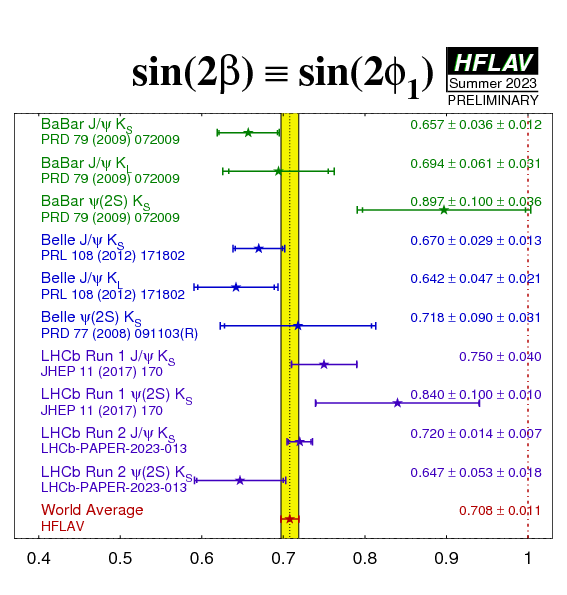
\includegraphics[width = 1.0\textwidth]{Plots/btoccsS_CP_woImprecise.png}
    \end{subfigure}
  \end{figure}
  \vspace{-0.5cm}
  \begin{center}
    \Large World average: $\sin(2\beta) = 0.708 \pm 0.011$\\
    \Large $\beta = (22.5 \pm 0.4)^\circ$
  \end{center}
\end{frame}

\begin{frame}{The CKM matrix and the Unitary Triangle}
  \begin{center}
    \Large From $B^0$/$B^0_s$ mixing, $\lvert V_{td}^{\phantom{*}}V_{tb}^*\rvert$ is measured\\
    \large This is dominated by lattice QCD uncertainties
  \end{center}
  \vspace{-0.3cm}
  \begin{figure}
    \centering
    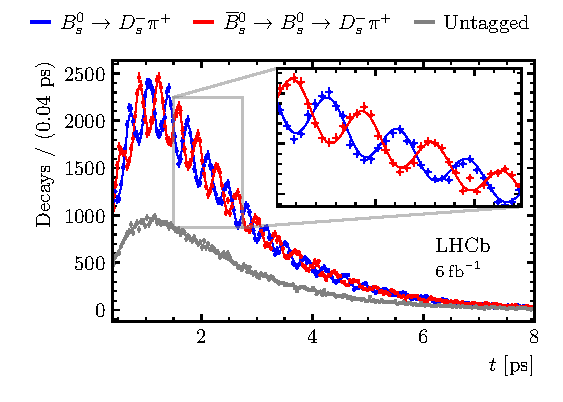
\includegraphics[width = 0.6\textwidth]{Plots/Bs_mixing.pdf}
    \vspace{-0.8cm}
    \caption*{\tiny Nature Physics \textbf{18}, (2022) 1}
  \end{figure}
  \vspace{-0.8cm}
  \begin{center}
    \Large HFLAV averages:\\
    \large $\Delta m_d = \SI{0.5065(19)}{\per\pico\second}$ \& $\Delta m_s = \SI{17.765(6)}{\per\pico\second}$
  \end{center}
\end{frame}

% TODO: This slide is a block of text
\begin{frame}{The CKM matrix and the Unitary Triangle}
  \begin{center}
    {\Large Why is the CKM angle $\gamma$ of interest?}
  \end{center}
  \begin{enumerate}
    \setlength\itemsep{0.0em}
    \item{Negligible theoretical uncertainties: Ideal SM benchmark}
    \begin{itemize}
      \item{Hadronic parameters are free parameters}
    \end{itemize}
    \item{Only CKM angle accessible in tree level decays}
    \begin{itemize}
      \item{Don't expect new physics at tree level, new particles appear in loops}
    \end{itemize}
    \item{We want to \underline{overconstrain} the Unitary Triangle}
  \end{enumerate}
  \vspace{-0.2cm}
  \begin{figure}
    \centering
    \begin{subfigure}{0.5\textwidth}
      \centering
      \begin{overpic}[width = 1.0\textwidth]{Plots/ckmfitter_loop.png}
        \put(100,28){\vector(-1.0,-0.25){55}}
        \put(100,30){Dominated by}
        \put(100,22){lattice QCD}
      \end{overpic}
      \caption*{Loop level: \colorbox{Cerulean!30}{$\gamma = \big(65.5^{+1.1}_{-2.7}\big)^\circ$}}
    \end{subfigure}
    \vspace{-0.3cm}
    \captionsetup{justification=centering}
    \caption*{\centering\tiny CKMfitter Group (J. Charles et al.), Eur. Phys. J. C41, 1-131 (2005), updated results and plots available at: \href{http://ckmfitter.in2p3.fr}{http://ckmfitter.in2p3.fr}}
  \end{figure}
  \vspace{-0.7cm}
  \begin{center}
    With precise $\gamma$ measurements, we can compare with the indirect loop level measurements, which assume unitarity (``SM prediction'')
  \end{center}
\end{frame}

\begin{frame}{The LHCb detector}
  \begin{center}
    {\huge The LHCb detector}\\~\\
    {\large (Original Run 1 and 2 detector)}
  \end{center}
\end{frame}

\begin{frame}{The LHCb detector}
  \begin{figure}
    \centering
    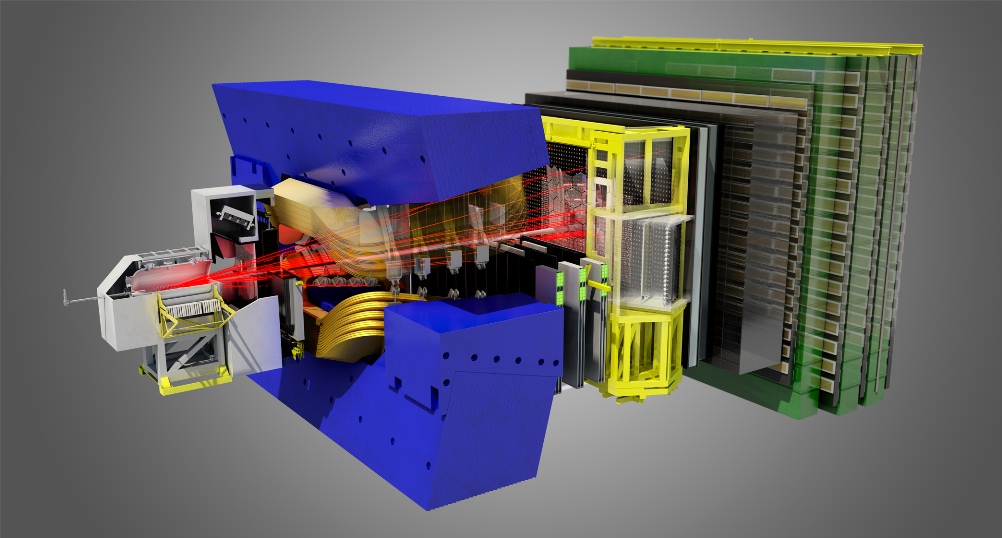
\includegraphics[width = 0.7\textwidth]{Plots/LHCbDetector.png}
  \end{figure}
  \begin{center}
    \Large LHCb: A beauty experiment with a lot of charm
  \end{center}
\end{frame}

\begin{frame}{The LHCb detector}
  \begin{figure}
    \centering
    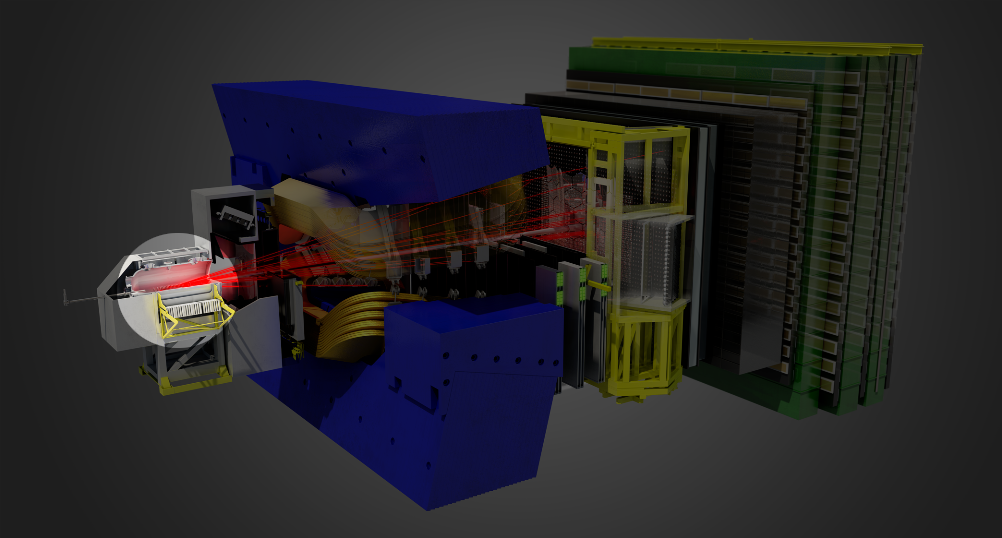
\includegraphics[width = 0.7\textwidth]{Plots/LHCbDetector_VELO.png}
  \end{figure}
  \begin{center}
    \Large VELO: Vertex locator to reconstruct $B$ and $D$ vertices\phantom{y}
  \end{center}
\end{frame}

\begin{frame}{The LHCb detector}
  \begin{figure}
    \centering
    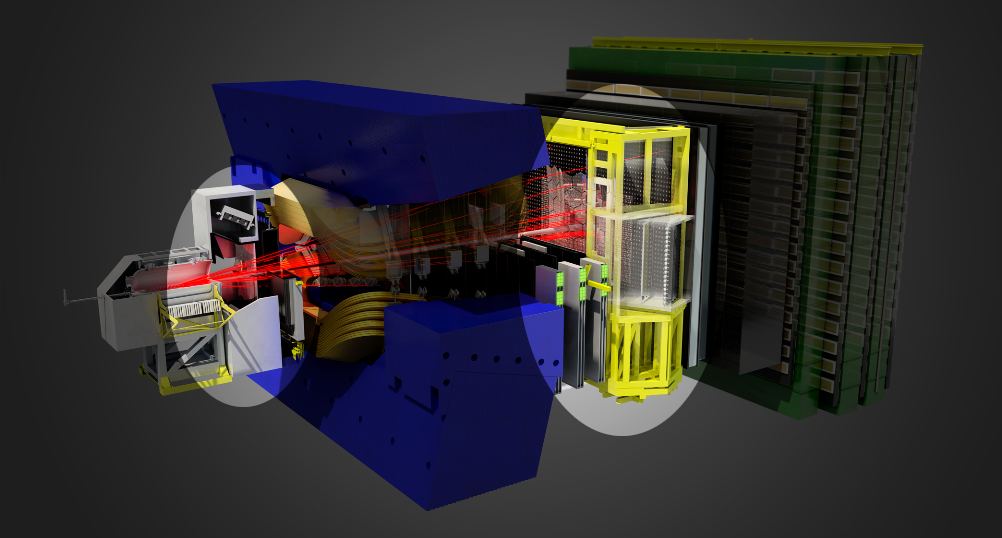
\includegraphics[width = 0.7\textwidth]{Plots/LHCbDetector_RICH.png}
  \end{figure}
  \begin{center}
    \Large RICH: Identify particles from $B$ and $D$
  \end{center}
\end{frame}

\section{How to measure \texorpdfstring{$\gamma$}{gamma}?}
\begin{frame}{How to measure $\gamma$?}
  \begin{center}
    {\huge How to measure $\gamma$?}\\~\\
    {\large It's all about interferences!}
  \end{center}
\end{frame}

\begin{frame}[fragile]{Sensitivity through interference}
  \begin{center}
    \Large Measure $\gamma$ through interference effects in $B^\pm\to DK^\pm$
  \end{center}
  \begin{figure}[H]
    \centering
    \begin{subfigure}{0.5\textwidth}
      \centering
      \begin{fmffile}{fgraph/fgraph_BtoDK1}
        \setlength{\unitlength}{0.4cm}
        \begin{fmfgraph*}(6,6)
          \fmfstraight
          \fmfleft{i1,B,i2,t1,t2,t3,t9,t10}
          \fmfright{o1,D,o2,t4,t5,o3,K,o4}
          \fmflabel{$\bar{u}$}{i1}
          \fmflabel{$b$}{i2}
          \fmfv{l.d=20,l.a=180,l={$B^-$\mylbrace{30}{-8}}}{B}
          \fmflabel{$\bar{u}$}{o1}
          \fmflabel{$c$}{o2}
          \fmflabel{$\bar{u}$}{o3}
          \fmflabel{$s$}{o4}
          \fmfv{l.d=15,l.a=0,l={\myrbrace{30}{-12}}$D^0$}{D}
          \fmfv{l.d=15,l.a=0,l={\myrbrace{30}{11}}$K^-$}{K}
          \fmf{fermion}{o1,i1}
          \fmf{fermion,tension=1.5}{i2,v1}
          \fmf{fermion}{v1,o2}
          \fmf{phantom,tension=1.5}{t9,v2}
          \fmf{boson,label=$W$,label.side=left,tension=0}{v1,v2}
          \fmf{fermion}{v2,o4}
          \fmf{fermion}{o3,v2}
        \end{fmfgraph*}
      \end{fmffile}
      \vspace{0.5cm}
      \caption*{Favoured $B^-\to D^0K^-$}
    \end{subfigure}%
    \begin{subfigure}{0.5\textwidth}
      \centering
      \begin{fmffile}{fgraph/fgraph_BtoDK2}
        \setlength{\unitlength}{0.4cm}
        \begin{fmfgraph*}(6,6)
          \fmfstraight
          \fmfleft{i1,t1,t2,B,t9,t10,i2}
          \fmfright{o1,K,o2,t4,t5,o3,D,o4}
          \fmflabel{$\bar{u}$}{i1}
          \fmflabel{$b$}{i2}
          \fmfv{l.d=20,l.a=180,l={$B^-$\mylbrace{100}{-8}}}{B}
          \fmflabel{$\bar{u}$}{o1}
          \fmflabel{$s$}{o2}
          \fmflabel{$\bar{c}$}{o3}
          \fmflabel{$u$}{o4}
          \fmfv{l.d=15,l.a=0,l={\myrbrace{30}{13}}$\bar{D^0}$}{D}
          \fmfv{l.d=15,l.a=0,l={\myrbrace{30}{-13}}$K^-$}{K}
          \fmf{fermion}{o1,i1}
          \fmf{fermion,tension=1.5}{i2,v1}
          \fmf{fermion}{v1,o4}
          \fmf{phantom,tension=1.5}{t2,v2}
          \fmf{boson,label=$W$,label.side=left,tension=0}{v1,v2}
          \fmf{fermion}{v2,o2}
          \fmf{fermion}{o3,v2}
        \end{fmfgraph*}
      \end{fmffile}
      \vspace{0.5cm}
      \caption*{CKM$+$colour suppressed $B^-\to\bar{D^0}K^-$}
    \end{subfigure}
  \end{figure}
  \begin{center}
    {\large Interference when $D^0$ and $\bar{D^0}$ decay to a common final state $f_D$}
  \end{center}
  \vspace{-0.26cm}
  \begin{equation*}
    \begin{tikzcd}[column sep=huge,row sep=tiny]
      & D^0K^- \arrow[dr] & \\
      B^- \arrow[ur] \arrow[dr] & [5cm] & f_DK^- \\
      & \bar{D^0}K^- \arrow[ur] & \\
    \end{tikzcd}
  \end{equation*}
  \vspace{-0.4cm}
\end{frame}

\begin{frame}{Sensitivity through interference}
  \begin{center}
    \Large Measure $\gamma$ through interference effects in $B^\pm\to DK^\pm$
  \end{center}
  \begin{figure}[H]
    \centering
    \begin{subfigure}{0.5\textwidth}
      \centering
      \begin{fmffile}{fgraph/fgraph_BtoDK1}
        \setlength{\unitlength}{0.4cm}
        \begin{fmfgraph*}(6,6)
          \fmfstraight
          \fmfleft{i1,B,i2,t1,t2,t3,t9,t10}
          \fmfright{o1,D,o2,t4,t5,o3,K,o4}
          \fmflabel{$\bar{u}$}{i1}
          \fmflabel{$b$}{i2}
          \fmfv{l.d=20,l.a=180,l={$B^-$\mylbrace{30}{-8}}}{B}
          \fmflabel{$\bar{u}$}{o1}
          \fmflabel{$c$}{o2}
          \fmflabel{$\bar{u}$}{o3}
          \fmflabel{$s$}{o4}
          \fmfv{l.d=15,l.a=0,l={\myrbrace{30}{-12}}$D^0$}{D}
          \fmfv{l.d=15,l.a=0,l={\myrbrace{30}{11}}$K^-$}{K}
          \fmf{fermion}{o1,i1}
          \fmf{fermion,tension=1.5}{i2,v1}
          \fmf{fermion}{v1,o2}
          \fmf{phantom,tension=1.5}{t9,v2}
          \fmf{boson,label=$W$,label.side=left,tension=0}{v1,v2}
          \fmf{fermion}{v2,o4}
          \fmf{fermion}{o3,v2}
        \end{fmfgraph*}
      \end{fmffile}
      \vspace{0.5cm}
      \caption*{Favoured $B^-\to D^0K^-$}
    \end{subfigure}%
    \begin{subfigure}{0.5\textwidth}
      \centering
      \begin{fmffile}{fgraph/fgraph_BtoDK2}
        \setlength{\unitlength}{0.4cm}
        \begin{fmfgraph*}(6,6)
          \fmfstraight
          \fmfleft{i1,t1,t2,B,t9,t10,i2}
          \fmfright{o1,K,o2,t4,t5,o3,D,o4}
          \fmflabel{$\bar{u}$}{i1}
          \fmflabel{$b$}{i2}
          \fmfv{l.d=20,l.a=180,l={$B^-$\mylbrace{100}{-8}}}{B}
          \fmflabel{$\bar{u}$}{o1}
          \fmflabel{$s$}{o2}
          \fmflabel{$\bar{c}$}{o3}
          \fmflabel{$u$}{o4}
          \fmfv{l.d=15,l.a=0,l={\myrbrace{30}{13}}$\bar{D^0}$}{D}
          \fmfv{l.d=15,l.a=0,l={\myrbrace{30}{-13}}$K^-$}{K}
          \fmf{fermion}{o1,i1}
          \fmf{fermion,tension=1.5}{i2,v1}
          \fmf{fermion}{v1,o4}
          \fmf{phantom,tension=1.5}{t2,v2}
          \fmf{boson,label=$W$,label.side=left,tension=0}{v1,v2}
          \fmf{fermion}{v2,o2}
          \fmf{fermion}{o3,v2}
        \end{fmfgraph*}
      \end{fmffile}
      \vspace{0.5cm}
      \caption*{CKM$+$colour suppressed $B^-\to\bar{D^0}K^-$}
    \end{subfigure}
  \end{figure}
  \vspace{-0.3cm}
  \begin{center}
    $b\to u\bar{c}s$ and $b\to c\bar{u}s$ interference $\to$ Sensitivity to $\gamma$
  \end{center}
  \vspace{-0.3cm}
  \begin{center}
    $\mathcal{A}(B^-)=\mathcal{A}_B\big(\mathcal{A}_{D^0} + \colorbox{white}{$r_B$}e^{i(\scriptsize\colorbox{white}{$\delta_B$} - \colorbox{white}{$\gamma$})}\mathcal{A}_{\bar{D^0}}\big)$ \\
    $\mathcal{A}(B^+)=\mathcal{A}_B\big(\mathcal{A}_{\bar{D^0}} + \colorbox{white}{$r_B$}e^{i(\scriptsize\colorbox{white}{$\delta_B$} + \colorbox{white}{$\gamma$})}\mathcal{A}_{D^0}\big)$ \\
  \end{center}
  \vspace{-0.3cm}
  \begin{center}
    \phantom{The magnitude of interference effects governed by $r_B\approx0.1$}
  \end{center}
\end{frame}

\begin{frame}{Sensitivity through interference}
  \begin{center}
    \Large Measure $\gamma$ through interference effects in $B^\pm\to DK^\pm$
  \end{center}
  \begin{figure}[H]
    \centering
    \begin{subfigure}{0.5\textwidth}
      \centering
      \begin{fmffile}{fgraph/fgraph_BtoDK1}
        \setlength{\unitlength}{0.4cm}
        \begin{fmfgraph*}(6,6)
          \fmfstraight
          \fmfleft{i1,B,i2,t1,t2,t3,t9,t10}
          \fmfright{o1,D,o2,t4,t5,o3,K,o4}
          \fmflabel{$\bar{u}$}{i1}
          \fmflabel{$b$}{i2}
          \fmfv{l.d=20,l.a=180,l={$B^-$\mylbrace{30}{-8}}}{B}
          \fmflabel{$\bar{u}$}{o1}
          \fmflabel{$c$}{o2}
          \fmflabel{$\bar{u}$}{o3}
          \fmflabel{$s$}{o4}
          \fmfv{l.d=15,l.a=0,l={\myrbrace{30}{-12}}$D^0$}{D}
          \fmfv{l.d=15,l.a=0,l={\myrbrace{30}{11}}$K^-$}{K}
          \fmf{fermion}{o1,i1}
          \fmf{fermion,tension=1.5}{i2,v1}
          \fmf{fermion}{v1,o2}
          \fmf{phantom,tension=1.5}{t9,v2}
          \fmf{boson,label=$W$,label.side=left,tension=0}{v1,v2}
          \fmf{fermion}{v2,o4}
          \fmf{fermion}{o3,v2}
        \end{fmfgraph*}
      \end{fmffile}
      \vspace{0.5cm}
      \caption*{Favoured $B^-\to D^0K^-$}
    \end{subfigure}%
    \begin{subfigure}{0.5\textwidth}
      \centering
      \begin{fmffile}{fgraph/fgraph_BtoDK2}
        \setlength{\unitlength}{0.4cm}
        \begin{fmfgraph*}(6,6)
          \fmfstraight
          \fmfleft{i1,t1,t2,B,t9,t10,i2}
          \fmfright{o1,K,o2,t4,t5,o3,D,o4}
          \fmflabel{$\bar{u}$}{i1}
          \fmflabel{$b$}{i2}
          \fmfv{l.d=20,l.a=180,l={$B^-$\mylbrace{100}{-8}}}{B}
          \fmflabel{$\bar{u}$}{o1}
          \fmflabel{$s$}{o2}
          \fmflabel{$\bar{c}$}{o3}
          \fmflabel{$u$}{o4}
          \fmfv{l.d=15,l.a=0,l={\myrbrace{30}{13}}$\bar{D^0}$}{D}
          \fmfv{l.d=15,l.a=0,l={\myrbrace{30}{-13}}$K^-$}{K}
          \fmf{fermion}{o1,i1}
          \fmf{fermion,tension=1.5}{i2,v1}
          \fmf{fermion}{v1,o4}
          \fmf{phantom,tension=1.5}{t2,v2}
          \fmf{boson,label=$W$,label.side=left,tension=0}{v1,v2}
          \fmf{fermion}{v2,o2}
          \fmf{fermion}{o3,v2}
        \end{fmfgraph*}
      \end{fmffile}
      \vspace{0.5cm}
      \caption*{CKM$+$colour suppressed $B^-\to\bar{D^0}K^-$}
    \end{subfigure}
  \end{figure}
  \vspace{-0.3cm}
  \begin{center}
    $b\to u\bar{c}s$ and $b\to c\bar{u}s$ interference $\to$ Sensitivity to $\gamma$
  \end{center}
  \vspace{-0.3cm}
  \begin{center}
    $\mathcal{A}(B^-)=\mathcal{A}_B\big(\mathcal{A}_{D^0} + \colorbox{Cerulean!30}{$r_B$}e^{i(\scriptsize\colorbox{white}{$\delta_B$} - \colorbox{white}{$\gamma$})}\mathcal{A}_{\bar{D^0}}\big)$ \\
    $\mathcal{A}(B^+)=\mathcal{A}_B\big(\mathcal{A}_{\bar{D^0}} + \colorbox{Cerulean!30}{$r_B$}e^{i(\scriptsize\colorbox{white}{$\delta_B$} + \colorbox{white}{$\gamma$})}\mathcal{A}_{D^0}\big)$ \\
  \end{center}
  \vspace{-0.3cm}
  \begin{center}
    The magnitude of interference effects governed by $r_B\approx0.1$
  \end{center}
\end{frame}

\begin{frame}{Sensitivity through interference}
  \begin{center}
    \Large Measure $\gamma$ through interference effects in $B^\pm\to DK^\pm$
  \end{center}
  \begin{figure}[H]
    \centering
    \begin{subfigure}{0.5\textwidth}
      \centering
      \begin{fmffile}{fgraph/fgraph_BtoDK1}
        \setlength{\unitlength}{0.4cm}
        \begin{fmfgraph*}(6,6)
          \fmfstraight
          \fmfleft{i1,B,i2,t1,t2,t3,t9,t10}
          \fmfright{o1,D,o2,t4,t5,o3,K,o4}
          \fmflabel{$\bar{u}$}{i1}
          \fmflabel{$b$}{i2}
          \fmfv{l.d=20,l.a=180,l={$B^-$\mylbrace{30}{-8}}}{B}
          \fmflabel{$\bar{u}$}{o1}
          \fmflabel{$c$}{o2}
          \fmflabel{$\bar{u}$}{o3}
          \fmflabel{$s$}{o4}
          \fmfv{l.d=15,l.a=0,l={\myrbrace{30}{-12}}$D^0$}{D}
          \fmfv{l.d=15,l.a=0,l={\myrbrace{30}{11}}$K^-$}{K}
          \fmf{fermion}{o1,i1}
          \fmf{fermion,tension=1.5}{i2,v1}
          \fmf{fermion}{v1,o2}
          \fmf{phantom,tension=1.5}{t9,v2}
          \fmf{boson,label=$W$,label.side=left,tension=0}{v1,v2}
          \fmf{fermion}{v2,o4}
          \fmf{fermion}{o3,v2}
        \end{fmfgraph*}
      \end{fmffile}
      \vspace{0.5cm}
      \caption*{Favoured $B^-\to D^0K^-$}
    \end{subfigure}%
    \begin{subfigure}{0.5\textwidth}
      \centering
      \begin{fmffile}{fgraph/fgraph_BtoDK2}
        \setlength{\unitlength}{0.4cm}
        \begin{fmfgraph*}(6,6)
          \fmfstraight
          \fmfleft{i1,t1,t2,B,t9,t10,i2}
          \fmfright{o1,K,o2,t4,t5,o3,D,o4}
          \fmflabel{$\bar{u}$}{i1}
          \fmflabel{$b$}{i2}
          \fmfv{l.d=20,l.a=180,l={$B^-$\mylbrace{100}{-8}}}{B}
          \fmflabel{$\bar{u}$}{o1}
          \fmflabel{$s$}{o2}
          \fmflabel{$\bar{c}$}{o3}
          \fmflabel{$u$}{o4}
          \fmfv{l.d=15,l.a=0,l={\myrbrace{30}{13}}$\bar{D^0}$}{D}
          \fmfv{l.d=15,l.a=0,l={\myrbrace{30}{-13}}$K^-$}{K}
          \fmf{fermion}{o1,i1}
          \fmf{fermion,tension=1.5}{i2,v1}
          \fmf{fermion}{v1,o4}
          \fmf{phantom,tension=1.5}{t2,v2}
          \fmf{boson,label=$W$,label.side=left,tension=0}{v1,v2}
          \fmf{fermion}{v2,o2}
          \fmf{fermion}{o3,v2}
        \end{fmfgraph*}
      \end{fmffile}
      \vspace{0.5cm}
      \caption*{CKM$+$colour suppressed $B^-\to\bar{D^0}K^-$}
    \end{subfigure}
  \end{figure}
  \vspace{-0.3cm}
  \begin{center}
    $b\to u\bar{c}s$ and $b\to c\bar{u}s$ interference $\to$ Sensitivity to $\gamma$
  \end{center}
  \vspace{-0.3cm}
  \begin{center}
    $\mathcal{A}(B^-)=\mathcal{A}_B\big(\mathcal{A}_{D^0} + \colorbox{white}{$r_B$}e^{i(\scriptsize\colorbox{Cerulean!30}{$\delta_B$} - \colorbox{white}{$\gamma$})}\mathcal{A}_{\bar{D^0}}\big)$ \\
    $\mathcal{A}(B^+)=\mathcal{A}_B\big(\mathcal{A}_{\bar{D^0}} + \colorbox{white}{$r_B$}e^{i(\scriptsize\colorbox{Cerulean!30}{$\delta_B$} + \colorbox{white}{$\gamma$})}\mathcal{A}_{D^0}\big)$ \\
  \end{center}
  \vspace{-0.3cm}
  \begin{center}
    The strong-phase difference $\delta_B$ accounts for all unknown QCD phase shifts
  \end{center}
\end{frame}

\begin{frame}{Sensitivity through interference}
  \begin{center}
    \Large Measure $\gamma$ through interference effects in $B^\pm\to DK^\pm$
  \end{center}
  \begin{figure}[H]
    \centering
    \begin{subfigure}{0.5\textwidth}
      \centering
      \begin{fmffile}{fgraph/fgraph_BtoDK1}
        \setlength{\unitlength}{0.4cm}
        \begin{fmfgraph*}(6,6)
          \fmfstraight
          \fmfleft{i1,B,i2,t1,t2,t3,t9,t10}
          \fmfright{o1,D,o2,t4,t5,o3,K,o4}
          \fmflabel{$\bar{u}$}{i1}
          \fmflabel{$b$}{i2}
          \fmfv{l.d=20,l.a=180,l={$B^-$\mylbrace{30}{-8}}}{B}
          \fmflabel{$\bar{u}$}{o1}
          \fmflabel{$c$}{o2}
          \fmflabel{$\bar{u}$}{o3}
          \fmflabel{$s$}{o4}
          \fmfv{l.d=15,l.a=0,l={\myrbrace{30}{-12}}$D^0$}{D}
          \fmfv{l.d=15,l.a=0,l={\myrbrace{30}{11}}$K^-$}{K}
          \fmf{fermion}{o1,i1}
          \fmf{fermion,tension=1.5}{i2,v1}
          \fmf{fermion}{v1,o2}
          \fmf{phantom,tension=1.5}{t9,v2}
          \fmf{boson,label=$W$,label.side=left,tension=0}{v1,v2}
          \fmf{fermion}{v2,o4}
          \fmf{fermion}{o3,v2}
        \end{fmfgraph*}
      \end{fmffile}
      \vspace{0.5cm}
      \caption*{Favoured $B^-\to D^0K^-$}
    \end{subfigure}%
    \begin{subfigure}{0.5\textwidth}
      \centering
      \begin{fmffile}{fgraph/fgraph_BtoDK2}
        \setlength{\unitlength}{0.4cm}
        \begin{fmfgraph*}(6,6)
          \fmfstraight
          \fmfleft{i1,t1,t2,B,t9,t10,i2}
          \fmfright{o1,K,o2,t4,t5,o3,D,o4}
          \fmflabel{$\bar{u}$}{i1}
          \fmflabel{$b$}{i2}
          \fmfv{l.d=20,l.a=180,l={$B^-$\mylbrace{100}{-8}}}{B}
          \fmflabel{$\bar{u}$}{o1}
          \fmflabel{$s$}{o2}
          \fmflabel{$\bar{c}$}{o3}
          \fmflabel{$u$}{o4}
          \fmfv{l.d=15,l.a=0,l={\myrbrace{30}{13}}$\bar{D^0}$}{D}
          \fmfv{l.d=15,l.a=0,l={\myrbrace{30}{-13}}$K^-$}{K}
          \fmf{fermion}{o1,i1}
          \fmf{fermion,tension=1.5}{i2,v1}
          \fmf{fermion}{v1,o4}
          \fmf{phantom,tension=1.5}{t2,v2}
          \fmf{boson,label=$W$,label.side=left,tension=0}{v1,v2}
          \fmf{fermion}{v2,o2}
          \fmf{fermion}{o3,v2}
        \end{fmfgraph*}
      \end{fmffile}
      \vspace{0.5cm}
      \caption*{CKM$+$colour suppressed $B^-\to\bar{D^0}K^-$}
    \end{subfigure}
  \end{figure}
  \vspace{-0.3cm}
  \begin{center}
    $b\to u\bar{c}s$ and $b\to c\bar{u}s$ interference $\to$ Sensitivity to $\gamma$
  \end{center}
  \vspace{-0.3cm}
  \begin{center}
    $\mathcal{A}(B^-)=\mathcal{A}_B\big(\mathcal{A}_{D^0} + \colorbox{white}{$r_B$}e^{i(\scriptsize\colorbox{white}{$\delta_B$} - \colorbox{Cerulean!30}{$\gamma$})}\mathcal{A}_{\bar{D^0}}\big)$ \\
    $\mathcal{A}(B^+)=\mathcal{A}_B\big(\mathcal{A}_{\bar{D^0}} + \colorbox{white}{$r_B$}e^{i(\scriptsize\colorbox{white}{$\delta_B$} + \colorbox{Cerulean!30}{$\gamma$})}\mathcal{A}_{D^0}\big)$ \\
  \end{center}
  \vspace{-0.3cm}
  \begin{center}
    The weak phase $\gamma$ swaps sign under CP
  \end{center}
\end{frame}

\begin{frame}{Sensitivity through interference}
  \begin{center}
    \Large Measure $\gamma$ through interference effects in $B^\pm\to DK^\pm$
  \end{center}
  \begin{figure}[H]
    \centering
    \begin{subfigure}{0.5\textwidth}
      \centering
      \begin{fmffile}{fgraph/fgraph_BtoDK1}
        \setlength{\unitlength}{0.4cm}
        \begin{fmfgraph*}(6,6)
          \fmfstraight
          \fmfleft{i1,B,i2,t1,t2,t3,t9,t10}
          \fmfright{o1,D,o2,t4,t5,o3,K,o4}
          \fmflabel{$\bar{u}$}{i1}
          \fmflabel{$b$}{i2}
          \fmfv{l.d=20,l.a=180,l={$B^-$\mylbrace{30}{-8}}}{B}
          \fmflabel{$\bar{u}$}{o1}
          \fmflabel{$c$}{o2}
          \fmflabel{$\bar{u}$}{o3}
          \fmflabel{$s$}{o4}
          \fmfv{l.d=15,l.a=0,l={\myrbrace{30}{-12}}$D^0$}{D}
          \fmfv{l.d=15,l.a=0,l={\myrbrace{30}{11}}$K^-$}{K}
          \fmf{fermion}{o1,i1}
          \fmf{fermion,tension=1.5}{i2,v1}
          \fmf{fermion}{v1,o2}
          \fmf{phantom,tension=1.5}{t9,v2}
          \fmf{boson,label=$W$,label.side=left,tension=0}{v1,v2}
          \fmf{fermion}{v2,o4}
          \fmf{fermion}{o3,v2}
        \end{fmfgraph*}
      \end{fmffile}
      \vspace{0.5cm}
      \caption*{Favoured $B^-\to D^0K^-$}
    \end{subfigure}%
    \begin{subfigure}{0.5\textwidth}
      \centering
      \begin{fmffile}{fgraph/fgraph_BtoDK2}
        \setlength{\unitlength}{0.4cm}
        \begin{fmfgraph*}(6,6)
          \fmfstraight
          \fmfleft{i1,t1,t2,B,t9,t10,i2}
          \fmfright{o1,K,o2,t4,t5,o3,D,o4}
          \fmflabel{$\bar{u}$}{i1}
          \fmflabel{$b$}{i2}
          \fmfv{l.d=20,l.a=180,l={$B^-$\mylbrace{100}{-8}}}{B}
          \fmflabel{$\bar{u}$}{o1}
          \fmflabel{$s$}{o2}
          \fmflabel{$\bar{c}$}{o3}
          \fmflabel{$u$}{o4}
          \fmfv{l.d=15,l.a=0,l={\myrbrace{30}{13}}$\bar{D^0}$}{D}
          \fmfv{l.d=15,l.a=0,l={\myrbrace{30}{-13}}$K^-$}{K}
          \fmf{fermion}{o1,i1}
          \fmf{fermion,tension=1.5}{i2,v1}
          \fmf{fermion}{v1,o4}
          \fmf{phantom,tension=1.5}{t2,v2}
          \fmf{boson,label=$W$,label.side=left,tension=0}{v1,v2}
          \fmf{fermion}{v2,o2}
          \fmf{fermion}{o3,v2}
        \end{fmfgraph*}
      \end{fmffile}
      \vspace{0.5cm}
      \caption*{CKM$+$colour suppressed $B^-\to\bar{D^0}K^-$}
    \end{subfigure}
  \end{figure}
  \vspace{-0.3cm}
  \begin{center}
    $b\to u\bar{c}s$ and $b\to c\bar{u}s$ interference $\to$ Sensitivity to $\gamma$
  \end{center}
  \vspace{-0.3cm}
  \begin{center}
    $\mathcal{A}(B^-)=\mathcal{A}_B\big(\mathcal{A}_{D^0} + \colorbox{Cerulean!30}{$r_B$}e^{i(\scriptsize\colorbox{Cerulean!30}{$\delta_B$} - \colorbox{Cerulean!30}{$\gamma$})}\mathcal{A}_{\bar{D^0}}\big)$ \\
    $\mathcal{A}(B^+)=\mathcal{A}_B\big(\mathcal{A}_{\bar{D^0}} + \colorbox{Cerulean!30}{$r_B$}e^{i(\scriptsize\colorbox{Cerulean!30}{$\delta_B$} + \colorbox{Cerulean!30}{$\gamma$})}\mathcal{A}_{D^0}\big)$ \\
  \end{center}
  \vspace{-0.3cm}
  \begin{center}
    $\gamma$, $r_B$, $\delta_B$ are free parameters $\implies$ No need for inputs from theory
  \end{center}
\end{frame}

\begin{frame}{What $D$ final states?}
  \begin{center}
    \Large What $D$ final states should we consider?\\~\\
    \Large No single method is sufficient to determine $\gamma$ precisely!
  \end{center}
  \vspace{0.2cm}
  \begin{enumerate}
    \setlength\itemsep{1.0em}
    \item{GLW method: CP eigenstates}
    \begin{itemize}
      \item{$D\to K^+K^-$, $\pi^+\pi^-$, ...}
    \end{itemize}
    \item{\phantom{ADS method: Doubly-Cabibbo Suppressed decays}}
    \begin{itemize}
      \item[]{\phantom{$D\to K^-\pi^+$, $K^-\pi^+\pi^-\pi^+$, ...}}
    \end{itemize}
    \item{\phantom{BPGGSZ method: Multi-body final states}}
    \begin{itemize}
      \item[]{\phantom{$D\to K_S^0\pi^+\pi^-$, $K_S^0K^+K^-$, ...}}
    \end{itemize}
  \end{enumerate}
\end{frame}

\begin{frame}[fragile]{$D$ decays to a $C\!P$ eigenstate}
  \begin{center}
    Naively, we expect the size of CPV effects to be around $r_B\approx10\%$\\~\\
    For $C\!P$ eigenstates, $\mathcal{A}_{D^0} = \mathcal{A}_{\bar{D^0}}$
  \end{center}
  \begin{equation*}
    \begin{tikzcd}[column sep=huge]
      & D^0K^- \arrow[dr, bend left = 25, "\mathcal{A}_{D^0}"] & \\
      B^- \arrow[ur, bend left, line width = 1.7, "\mathcal{A}_B"] \arrow[dr, bend right, "\mathcal{A}_B r_B e^{i(\delta_B - \gamma)}"'] & [5cm] & DK^- \\
      & \bar{D^0}K^- \arrow[ur, bend right = 25, "\mathcal{A}_{D^0}"'] & \\
    \end{tikzcd}
  \end{equation*}
  \begin{equation*}
    \lvert\mathcal{A}(B^-)\lvert^2\propto1 + r_B^2 + 2r_B\cos(\delta_B - \gamma)
  \end{equation*}
\end{frame}

\begin{frame}{$D$ decays to a $C\!P$ eigenstate}
  \begin{figure}
    \centering
    \begin{subfigure}{0.45\textwidth}
      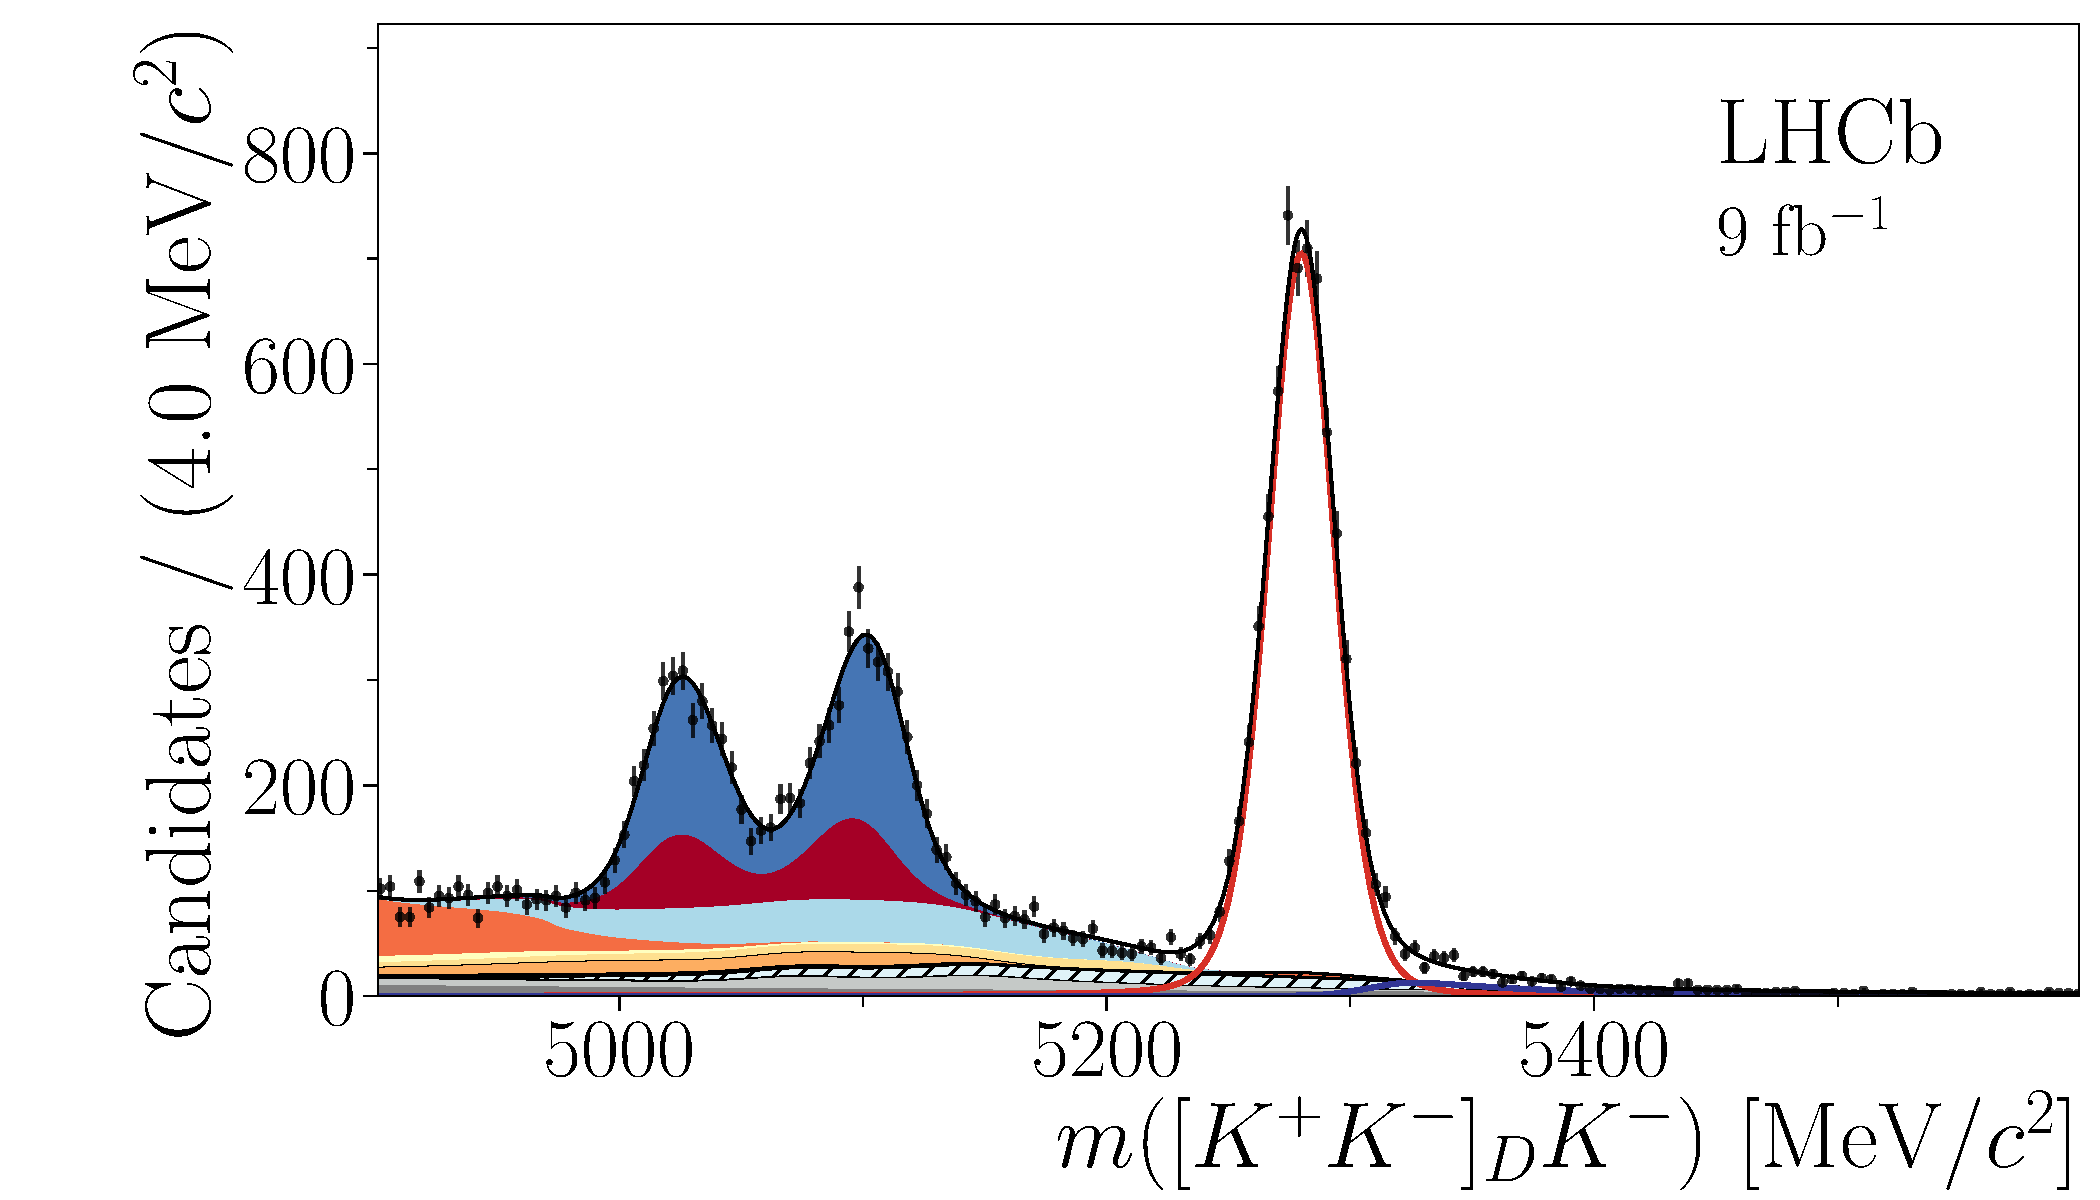
\includegraphics[width = 1.0\textwidth]{Plots/B2DK_D2KK_Minus.pdf}
    \end{subfigure}%
    \begin{subfigure}{0.45\textwidth}
      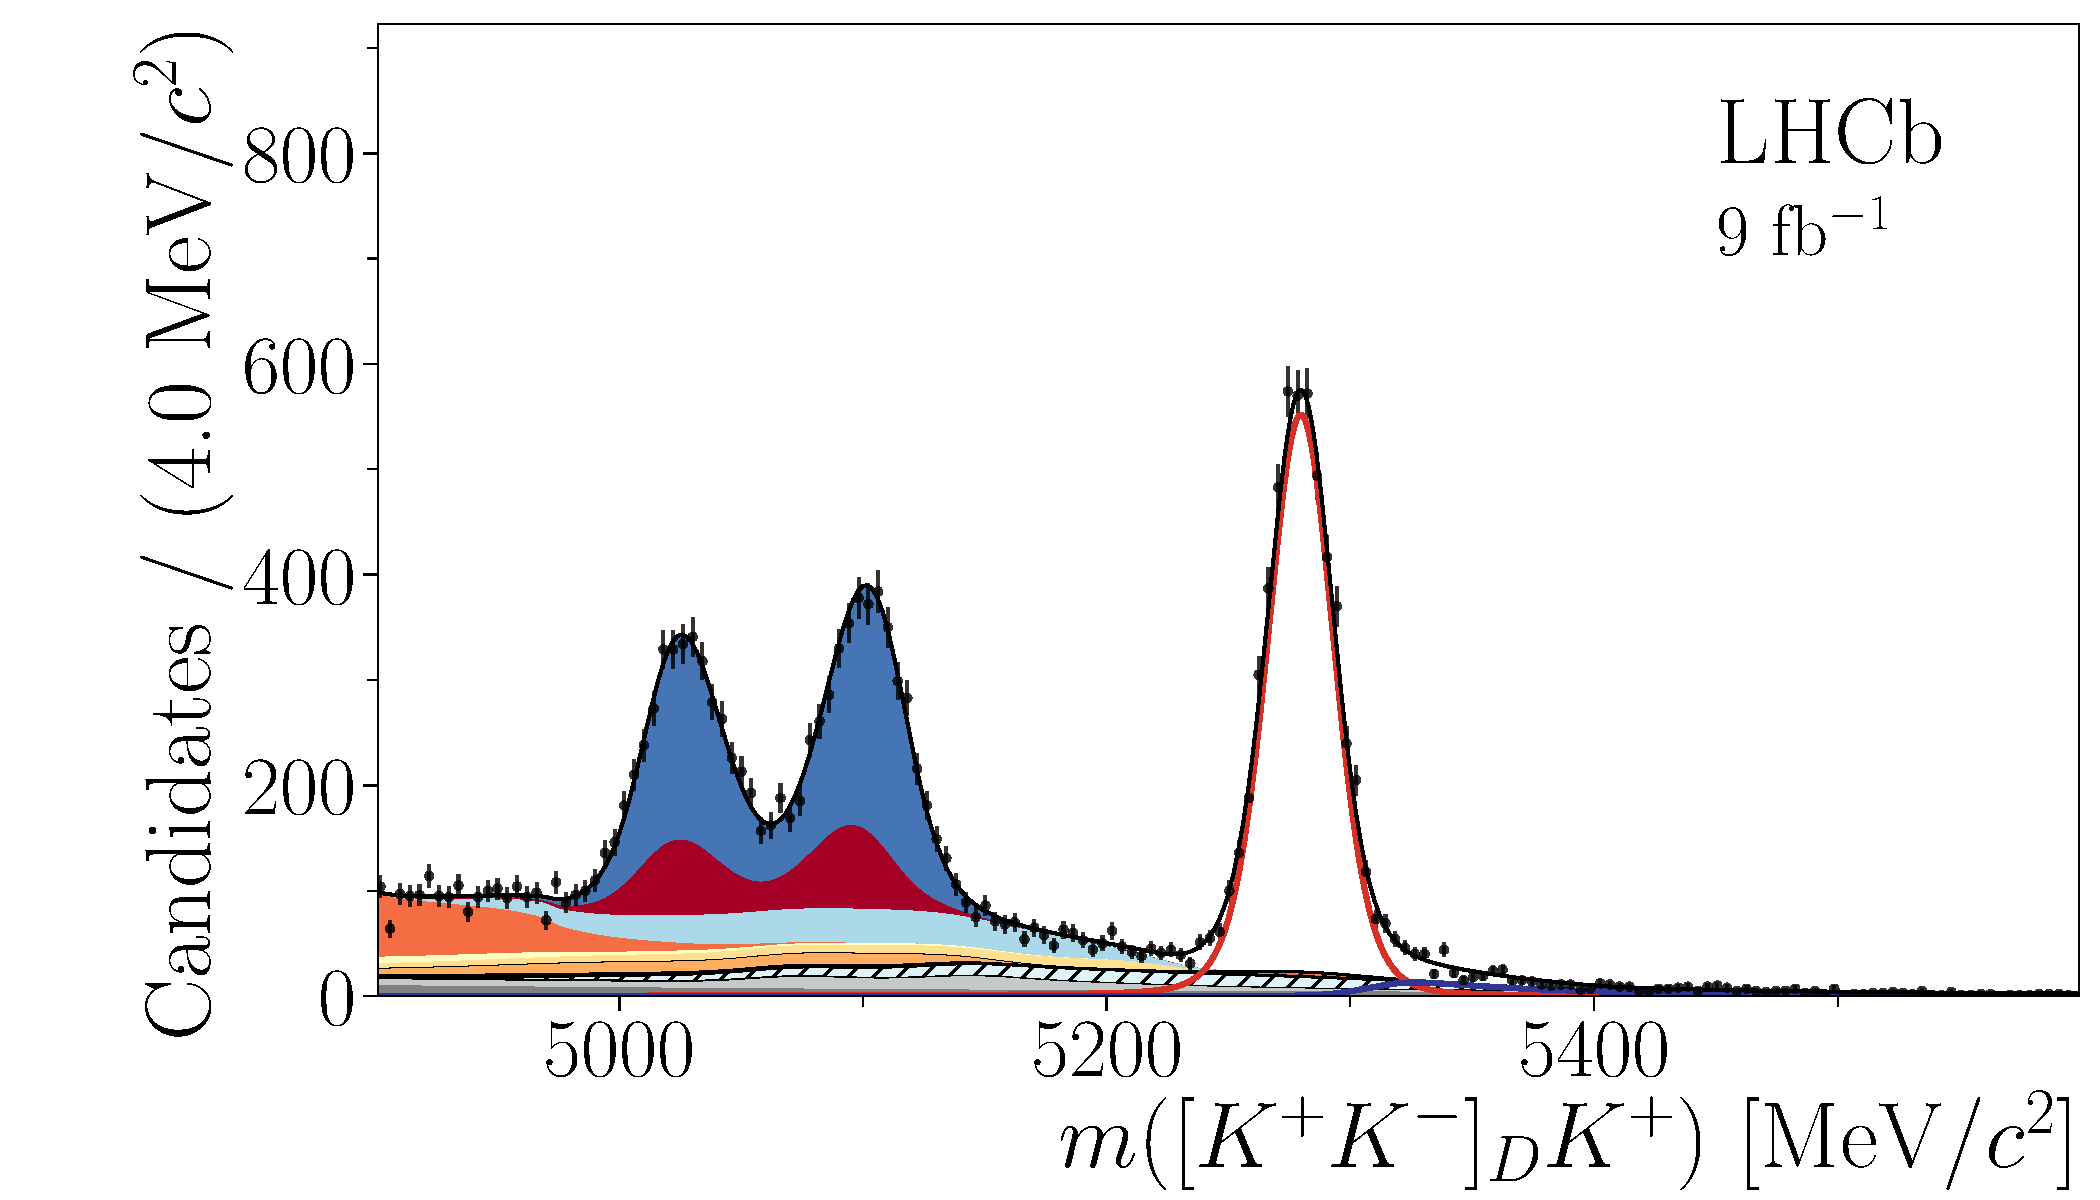
\includegraphics[width = 1.0\textwidth]{Plots/B2DK_D2KK_Plus.pdf}
    \end{subfigure}
    \begin{subfigure}{0.45\textwidth}
      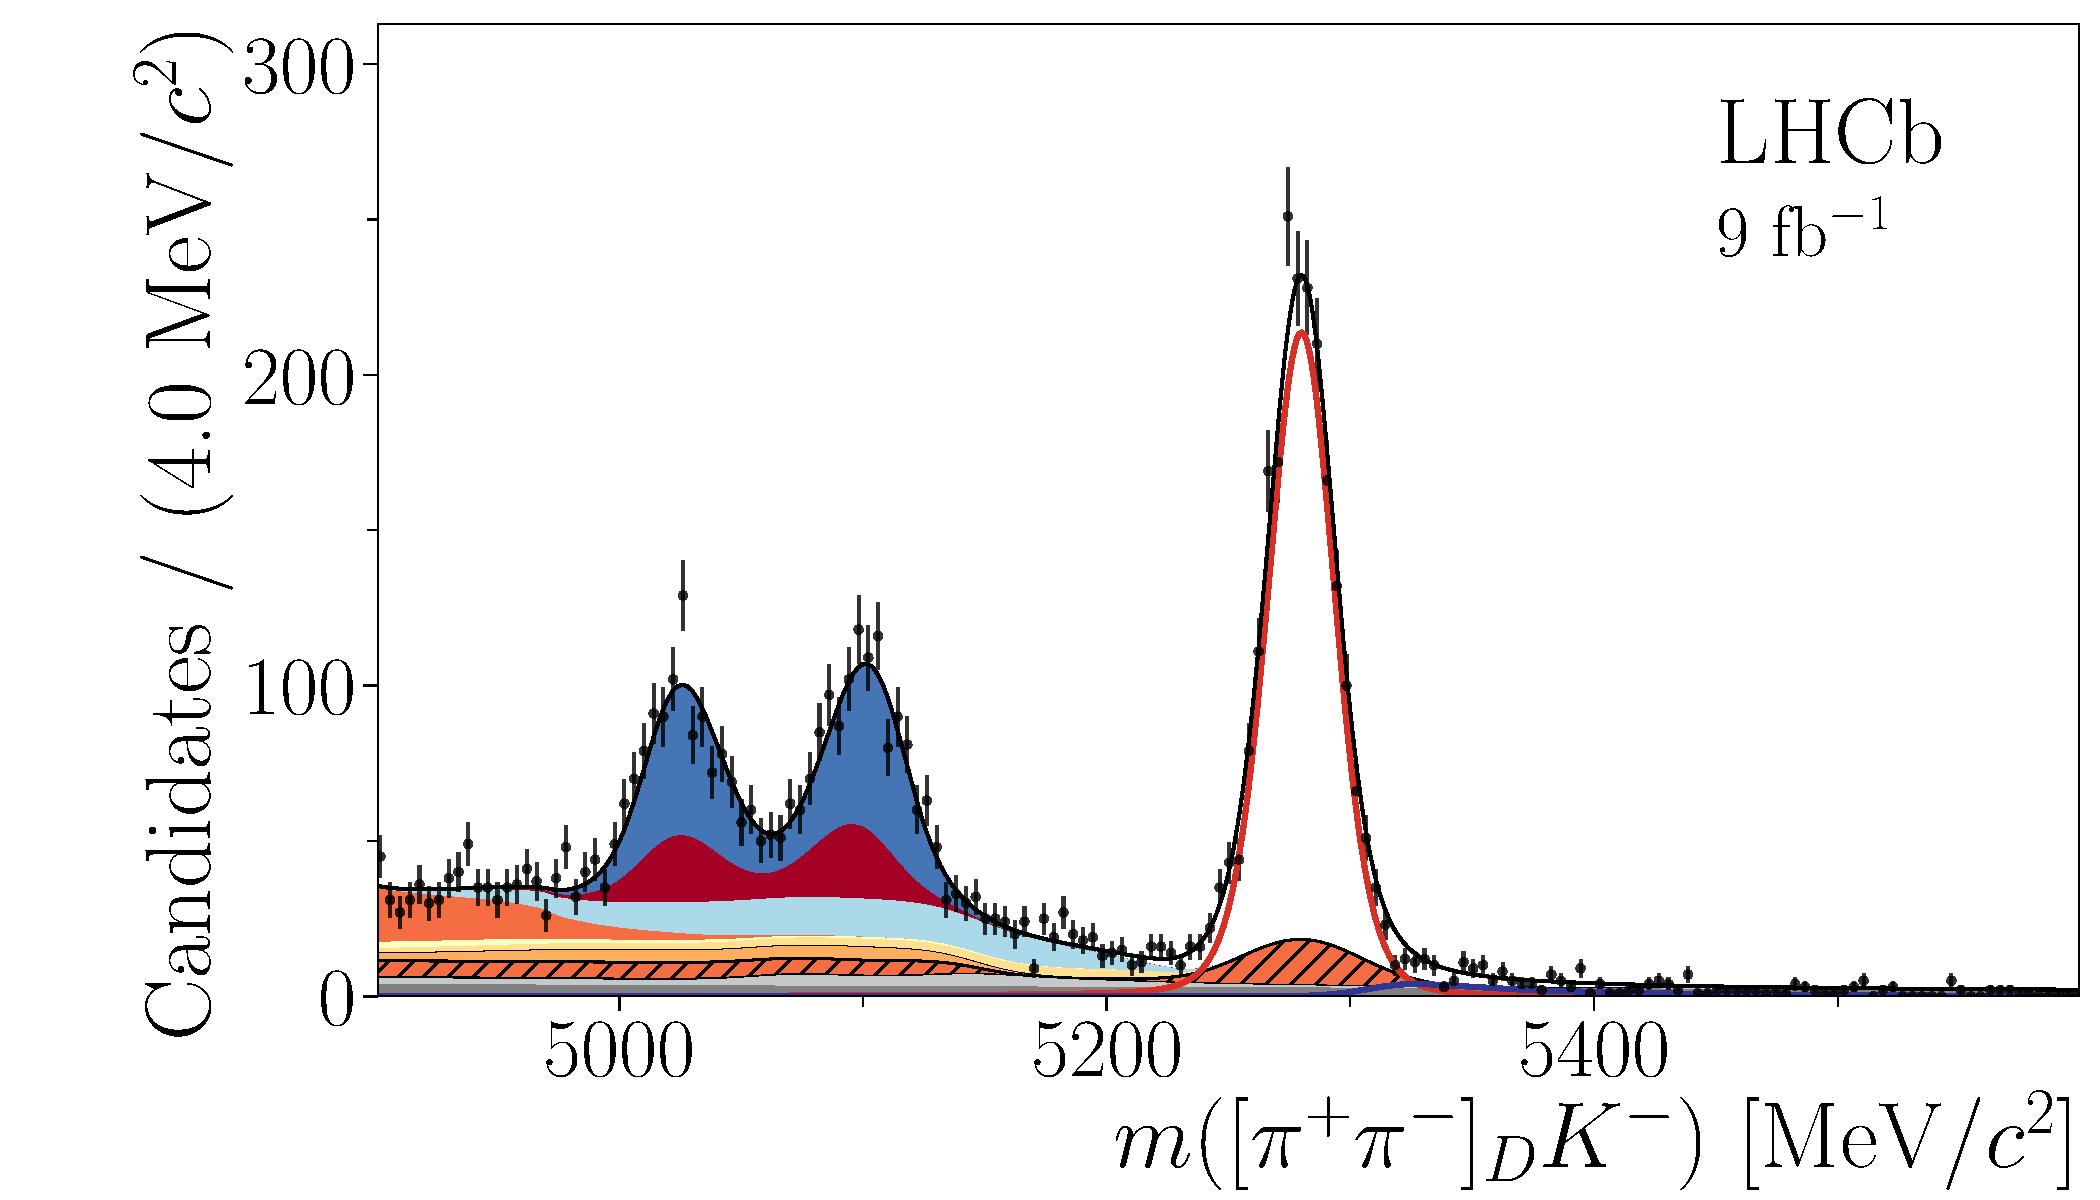
\includegraphics[width = 1.0\textwidth]{Plots/B2DK_D2pipi_Minus.pdf}
    \end{subfigure}%
    \begin{subfigure}{0.45\textwidth}
      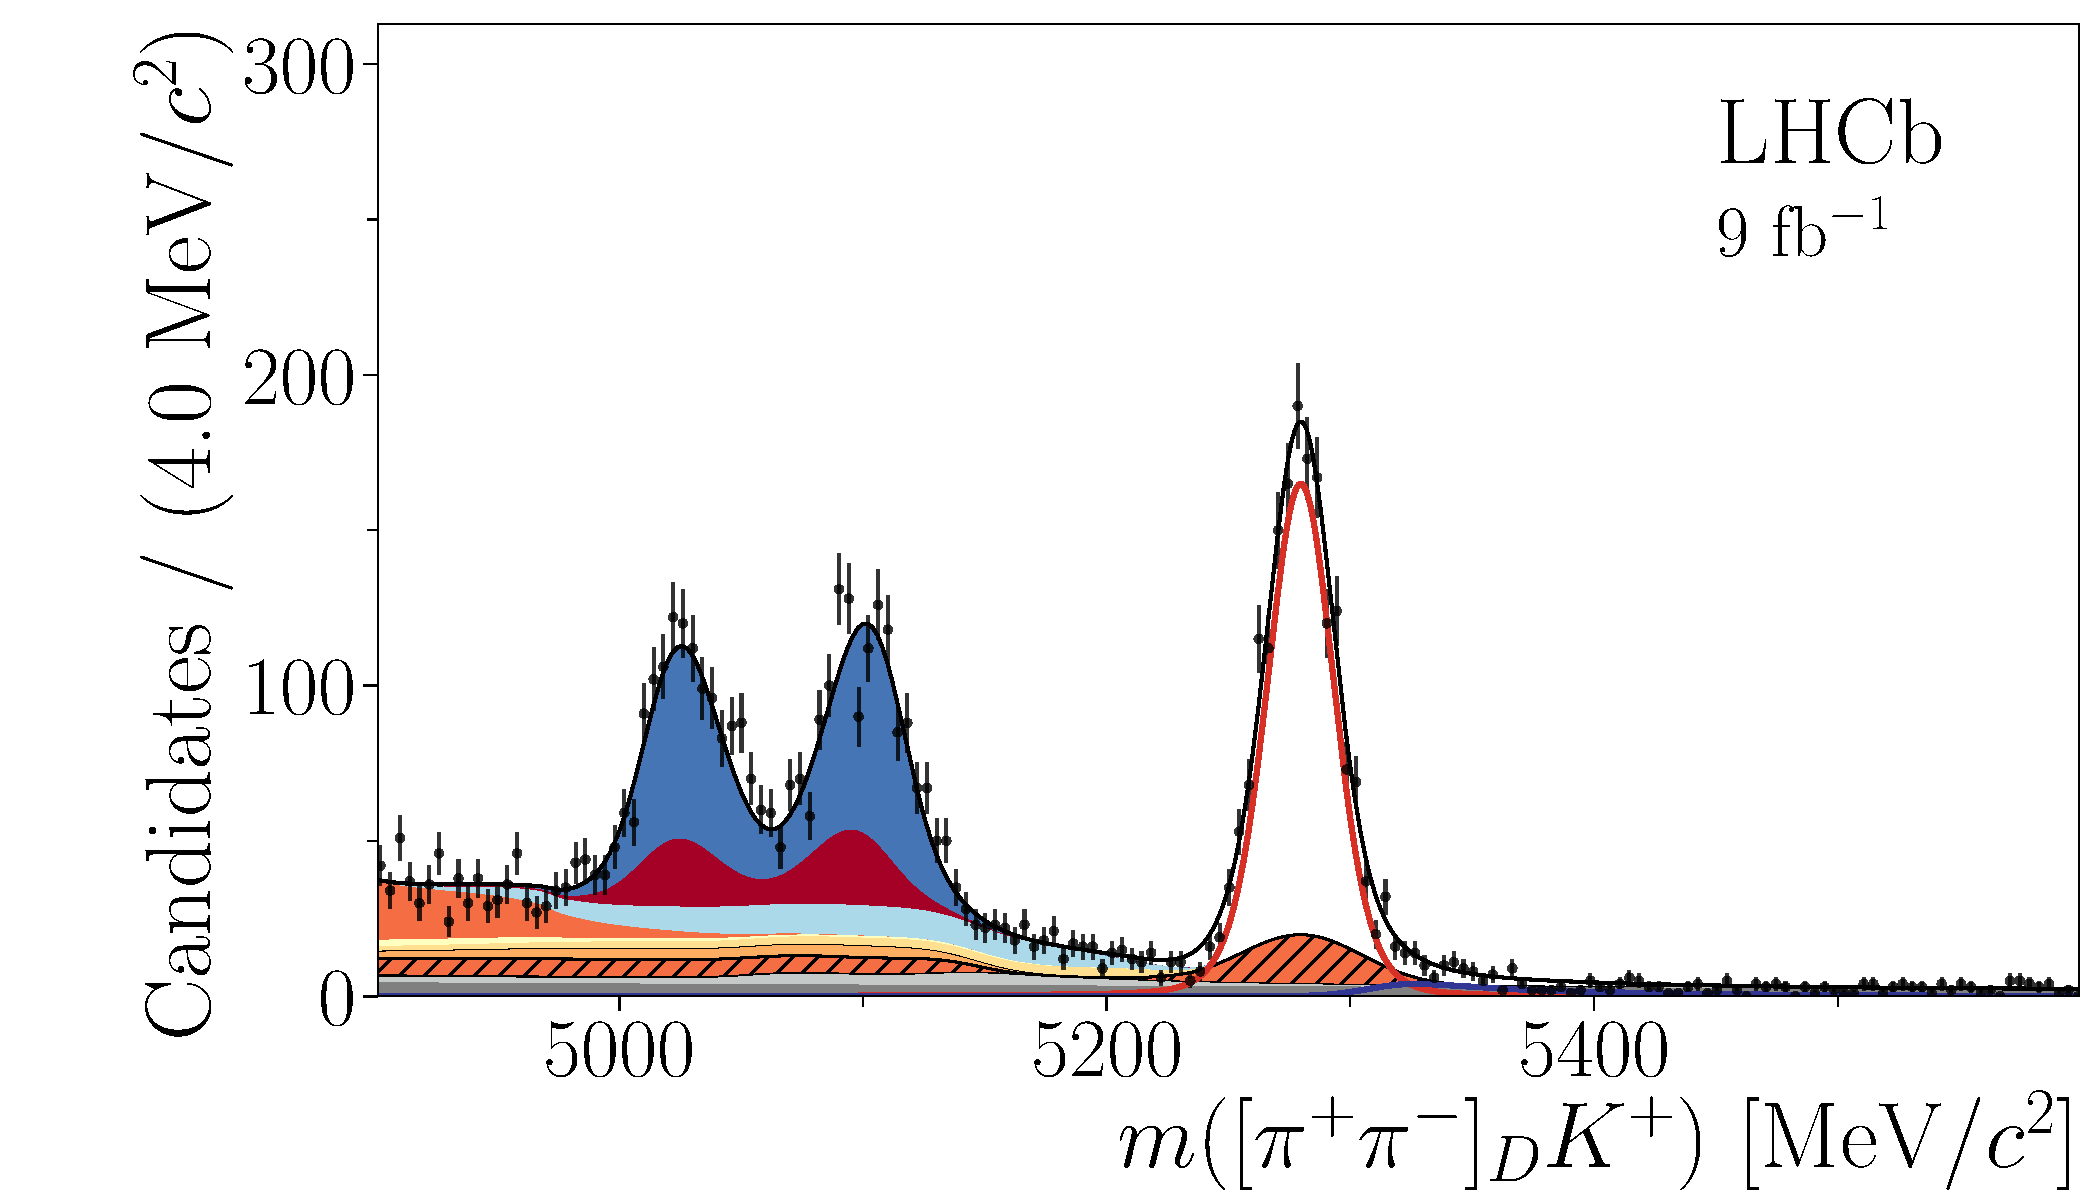
\includegraphics[width = 1.0\textwidth]{Plots/B2DK_D2pipi_Plus.pdf}
    \end{subfigure}
    \caption*{\tiny JHEP \textbf{04} (2021) 081}
  \end{figure}
  \vspace{-0.5cm}
  \begin{center}
    \Large In $B^\pm\to[h^+h^-]_DK^\pm$, we see significant CPV effects
  \end{center}
\end{frame}

\begin{frame}{What $D$ final states?}
  \begin{center}
    \Large What $D$ final states should we consider?\\~\\
    \Large No single method is sufficient to determine $\gamma$ precisely!
  \end{center}
  \vspace{0.2cm}
  \begin{enumerate}
    \setlength\itemsep{1.0em}
    \item{GLW method: CP eigenstates}
    \begin{itemize}
      \item{$D\to K^+K^-$, $\pi^+\pi^-$, ...}
    \end{itemize}
    \item{ADS method: Doubly-Cabibbo Suppressed decays}
    \begin{itemize}
      \item{$D\to K^-\pi^+$, $K^-\pi^+\pi^-\pi^+$, ...}
    \end{itemize}
    \item{\phantom{BPGGSZ method: Multi-body final states}}
    \begin{itemize}
      \item[]{\phantom{$D\to K_S^0\pi^+\pi^-$, $K_S^0K^+K^-$, ...}}
    \end{itemize}
  \end{enumerate}
\end{frame}

\begin{frame}[fragile]{Doubly Suppressed Cabibbo $D$ decays}
  \begin{center}
    Interference effects can be greatly enhanced\\~\\
    Use a Doubly Suppressed Cabibbo decay: $\mathcal{A}_{D^0} = r_De^{i\delta_D}\mathcal{A}_{\bar{D^0}}$
  \end{center}
  \begin{equation*}
    \begin{tikzcd}[column sep=huge]
      & D^0K^- \arrow[dr, bend left = 25, "r_De^{i\delta_D}\mathcal{A}_{\bar{D^0}}"] & \\
      B^- \arrow[ur, bend left, line width = 1.7, "\mathcal{A}_B"] \arrow[dr, bend right, "\mathcal{A}_B r_B e^{i(\delta_B - \gamma)}"'] & [5cm] & DK^- \\
      & \bar{D^0}K^- \arrow[ur, bend right = 25, line width = 1.7, "\mathcal{A}_{\bar{D^0}}"'] & \\
    \end{tikzcd}
  \end{equation*}
  \begin{equation*}
    \lvert\mathcal{A}(B^-)\lvert^2\propto r_D^2 + r_B^2 + 2r_Br_D\cos(\delta_B - \gamma + \delta_D)
  \end{equation*}
\end{frame}

\begin{frame}{Doubly Suppressed Cabibbo $D$ decays}
  \begin{figure}
    \centering
    \begin{subfigure}{0.5\textwidth}
      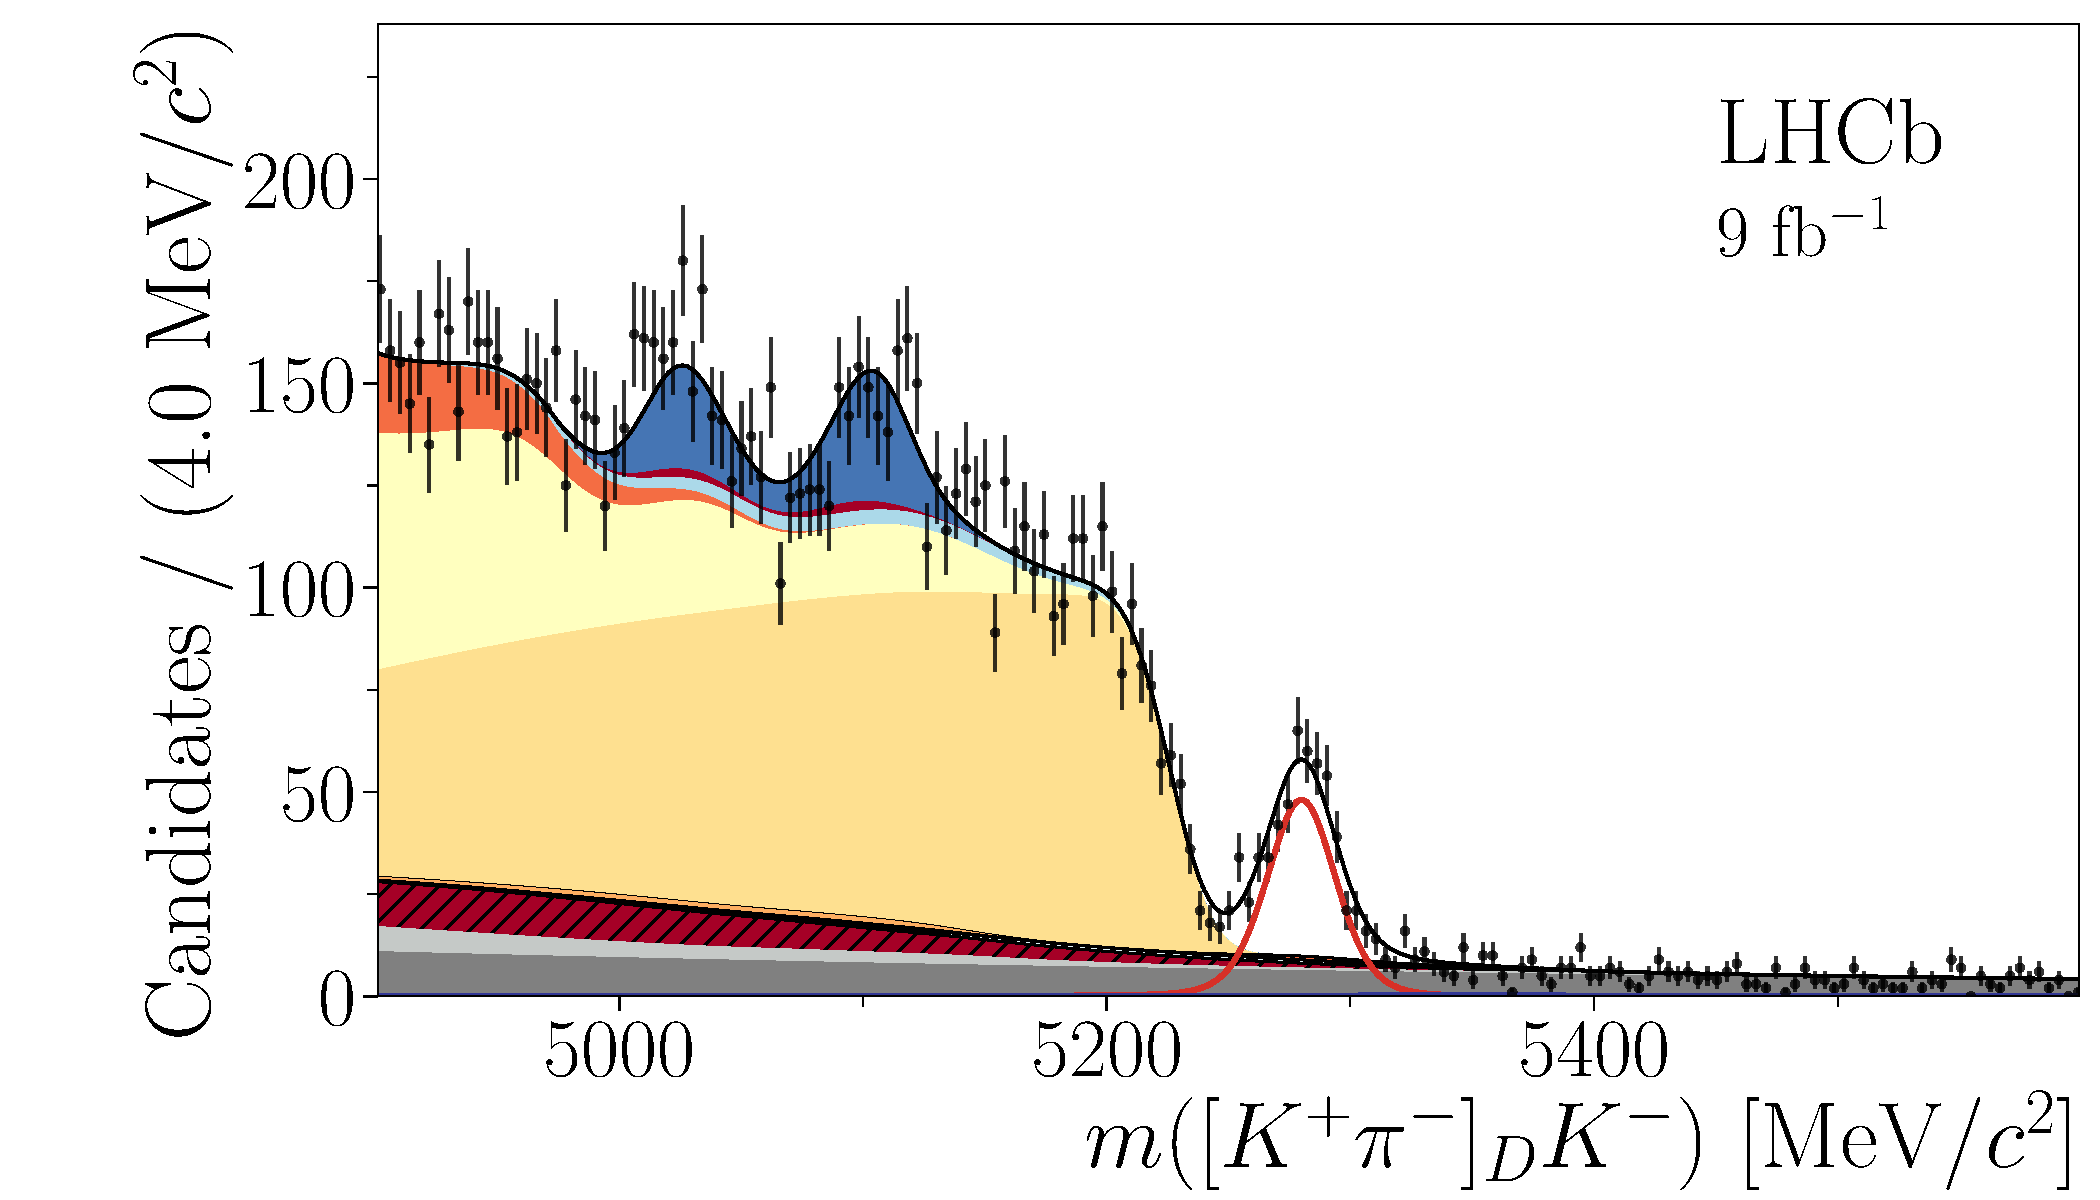
\includegraphics[width = 1.0\textwidth]{Plots/B2DK_D2Kpi_Minus.pdf}
    \end{subfigure}%
    \begin{subfigure}{0.5\textwidth}
      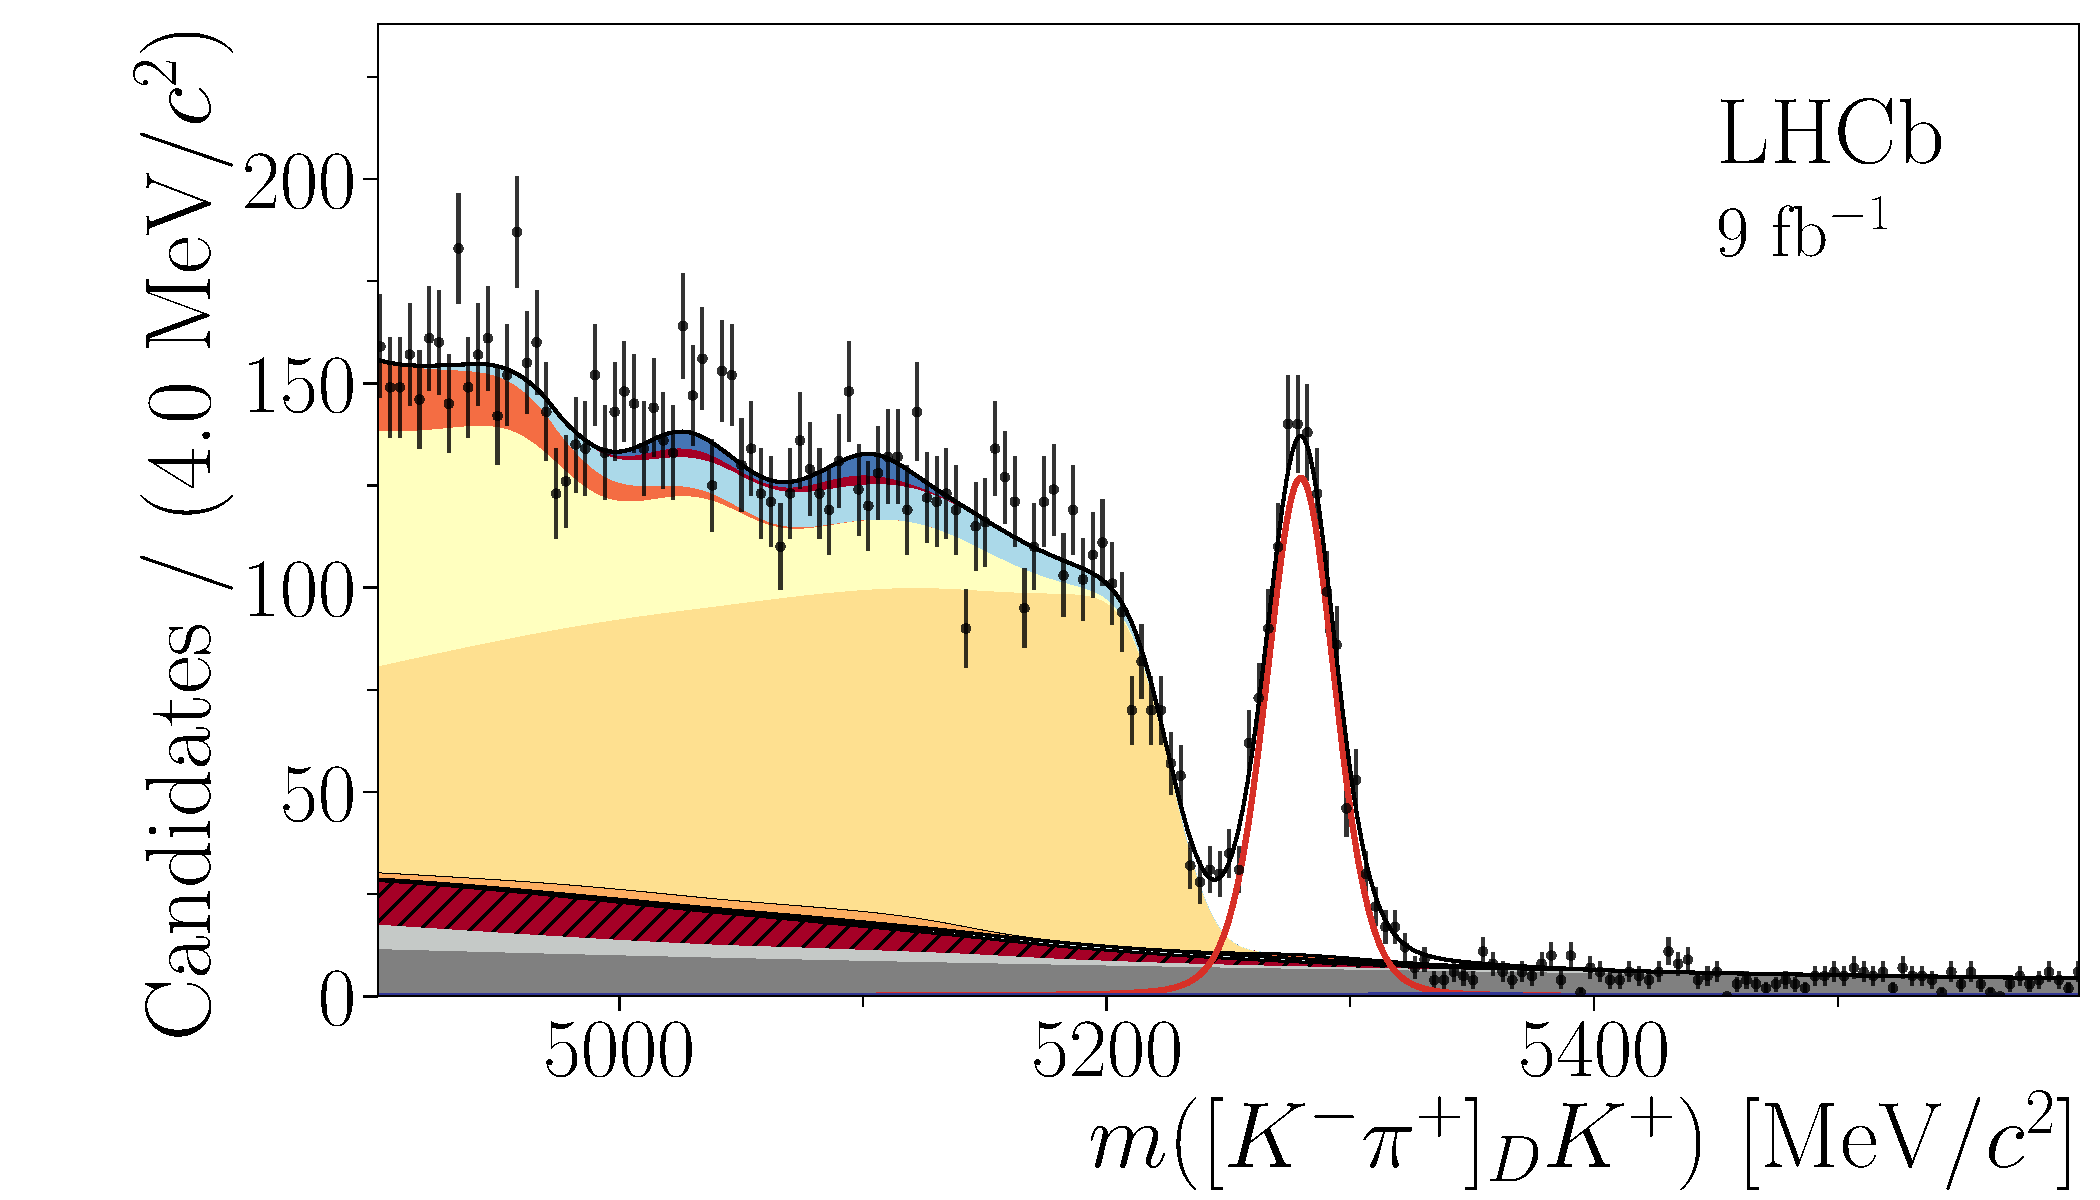
\includegraphics[width = 1.0\textwidth]{Plots/B2DK_D2Kpi_Plus.pdf}
    \end{subfigure}
    \caption*{\tiny JHEP \textbf{04} (2021) 081}
  \end{figure}
  \vspace{-0.5cm}
  \begin{center}
    \Large $B^\pm\to[K^\mp\pi^\pm]_DK^\pm$ has lower statistics, but a spectacular asymmetry!\\~\\
    \large Additionally, the partially reconstructed background has an equal but opposite asymmetry
  \end{center}
\end{frame}

\begin{frame}{What $D$ final states?}
  \begin{center}
    \Large What $D$ final states should we consider?\\~\\
    \Large No single method is sufficient to determine $\gamma$ precisely!
  \end{center}
  \vspace{0.2cm}
  \begin{enumerate}
    \setlength\itemsep{1.0em}
    \item{GLW method: CP eigenstates}
    \begin{itemize}
      \item{$D\to K^+K^-$, $\pi^+\pi^-$, ...}
    \end{itemize}
    \item{ADS method: Doubly-Cabibbo Suppressed decays}
    \begin{itemize}
      \item{$D\to K^-\pi^+$, $K^-\pi^+\pi^-\pi^+$, ...}
    \end{itemize}
    \item{BPGGSZ method: Multi-body final states}
    \begin{itemize}
      \item{$D\to K_S^0\pi^+\pi^-$, $K_S^0K^+K^-$, ...}
    \end{itemize}
  \end{enumerate}
\end{frame}

\begin{frame}[fragile]{Multi-body $D$ decays}
  \begin{center}
    The three-body $D$-decay phase space is two-dimensional $\implies$ Dalitz plot\\~\\
    $B^\pm$ decay rate depends on the $D^0$ and $\bar{D^0}$ strong-phase difference
  \end{center}
  \begin{equation*}
    \begin{tikzcd}[column sep=huge]
      & D^0K^- \arrow[dr, bend left = 25, dashed, "\mathcal{A}_{D^0}(\Phi)"] & \\
      B^- \arrow[ur, bend left, line width = 1.7, "\mathcal{A}_B"] \arrow[dr, bend right, "\mathcal{A}_B r_B e^{i(\delta_B - \gamma)}"'] & [5cm] & DK^- \\
      & \bar{D^0}K^- \arrow[ur, bend right = 25, dashed, "r_D(\Phi)e^{i\delta_D(\Phi)}\mathcal{A}_{D^0}(\Phi)"'] & \\
    \end{tikzcd}
  \end{equation*}
  \vspace{-0.5cm}
  \begin{equation*}
    \lvert\mathcal{A}(B^-)\lvert^2\propto1 + r_B^2r_D^2(\Phi) + 2r_Br_D(\Phi)\cos(\delta_B - \gamma + \delta_D(\Phi))
  \end{equation*}
\end{frame}

\begin{frame}{Multi-body $D$ decays}
  \begin{figure}
    \begin{subfigure}{0.5\textwidth}
      \begin{tikzpicture}
        \node(a){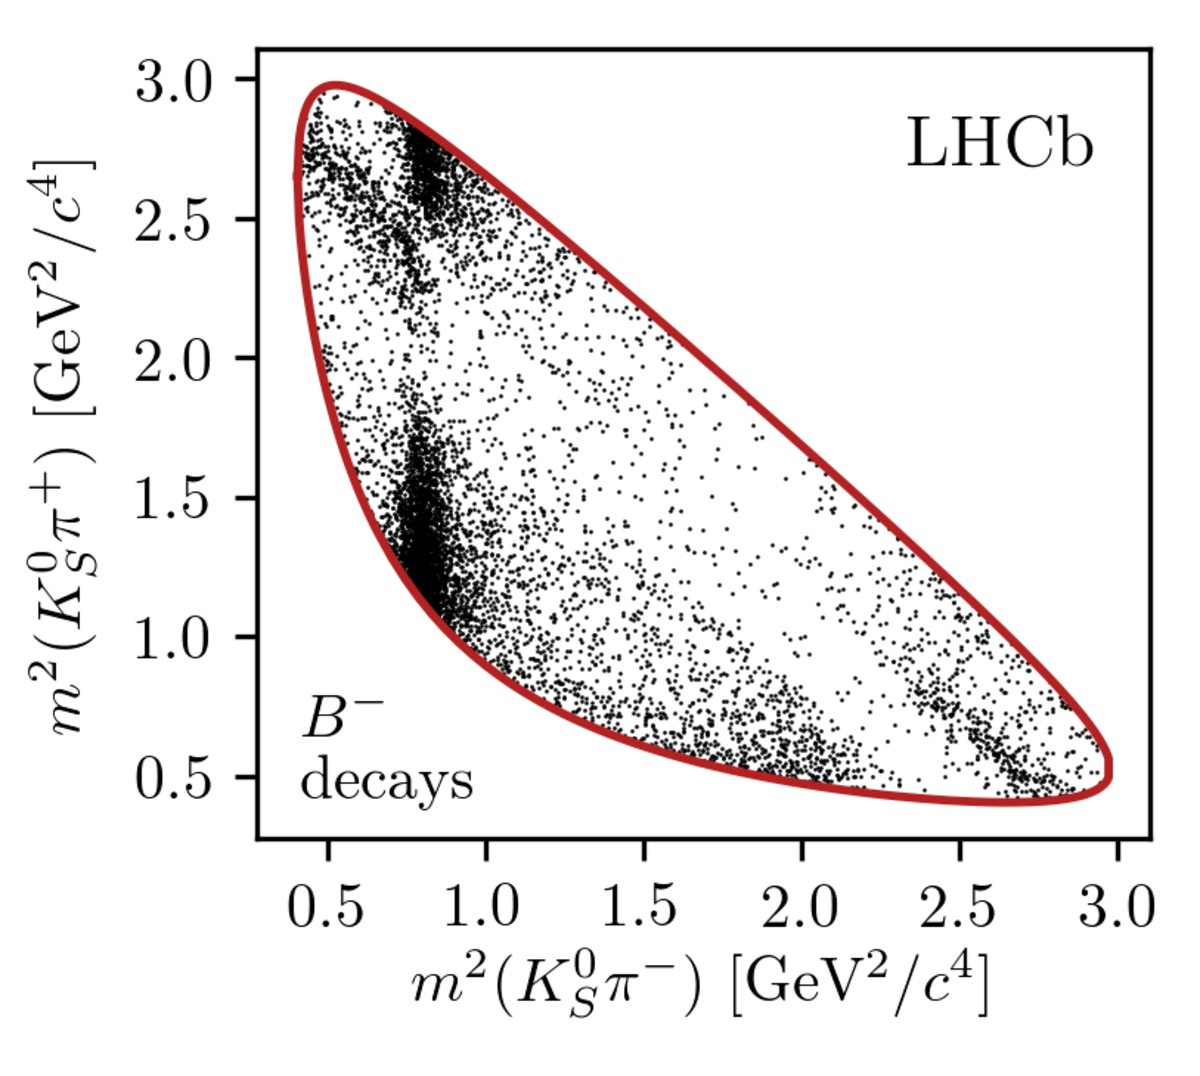
\includegraphics[width=1.0\textwidth]{Plots/KSpipi_Minus_Dalitz.png}};
      \end{tikzpicture}   
      \vspace{-0.8cm}
      \caption*{$B^-\to[K_S^0\pi^+\pi^-]_DK^-$}
    \end{subfigure}%
    \begin{subfigure}{0.5\textwidth}
      \begin{tikzpicture}
        \node(a){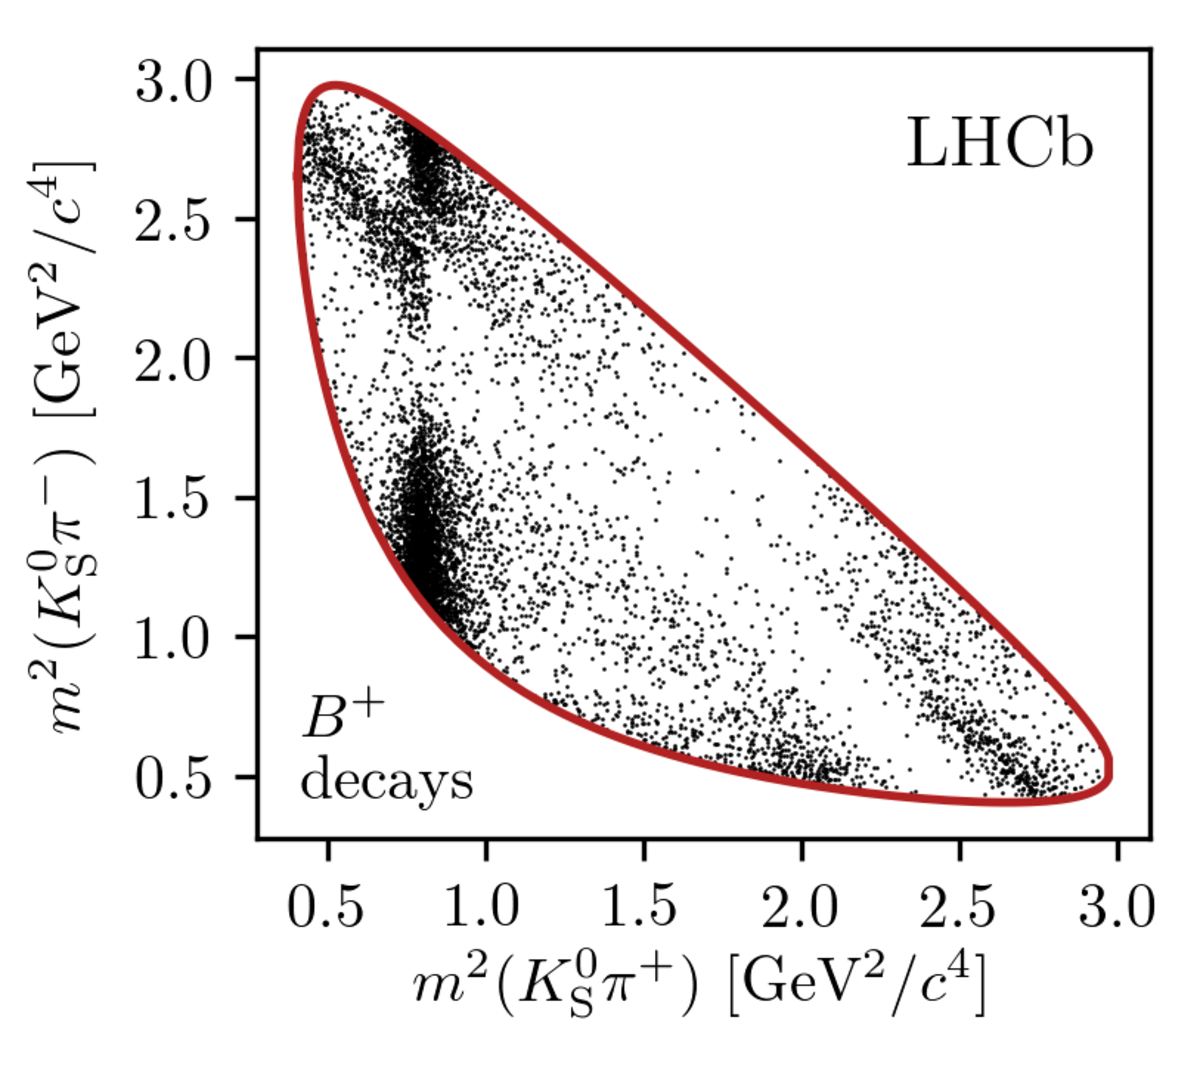
\includegraphics[width=1.0\textwidth]{Plots/KSpipi_Plus_Dalitz.png}};
      \end{tikzpicture}
      \vspace{-0.8cm}
      \caption*{$B^+\to[K_S^0\pi^+\pi^-]_DK^+$}
    \end{subfigure}
    \vspace{-0.3cm}
    \caption*{\tiny JHEP \textbf{02} (2021) 169}
  \end{figure}
  \vspace{-0.6cm}
  \begin{center}
    \Large Can you find the asymmetries?
  \end{center}
\end{frame}

\begin{frame}{Multi-body $D$ decays}
  \begin{figure}
    \begin{subfigure}{0.5\textwidth}
      \begin{tikzpicture}
        \node(a){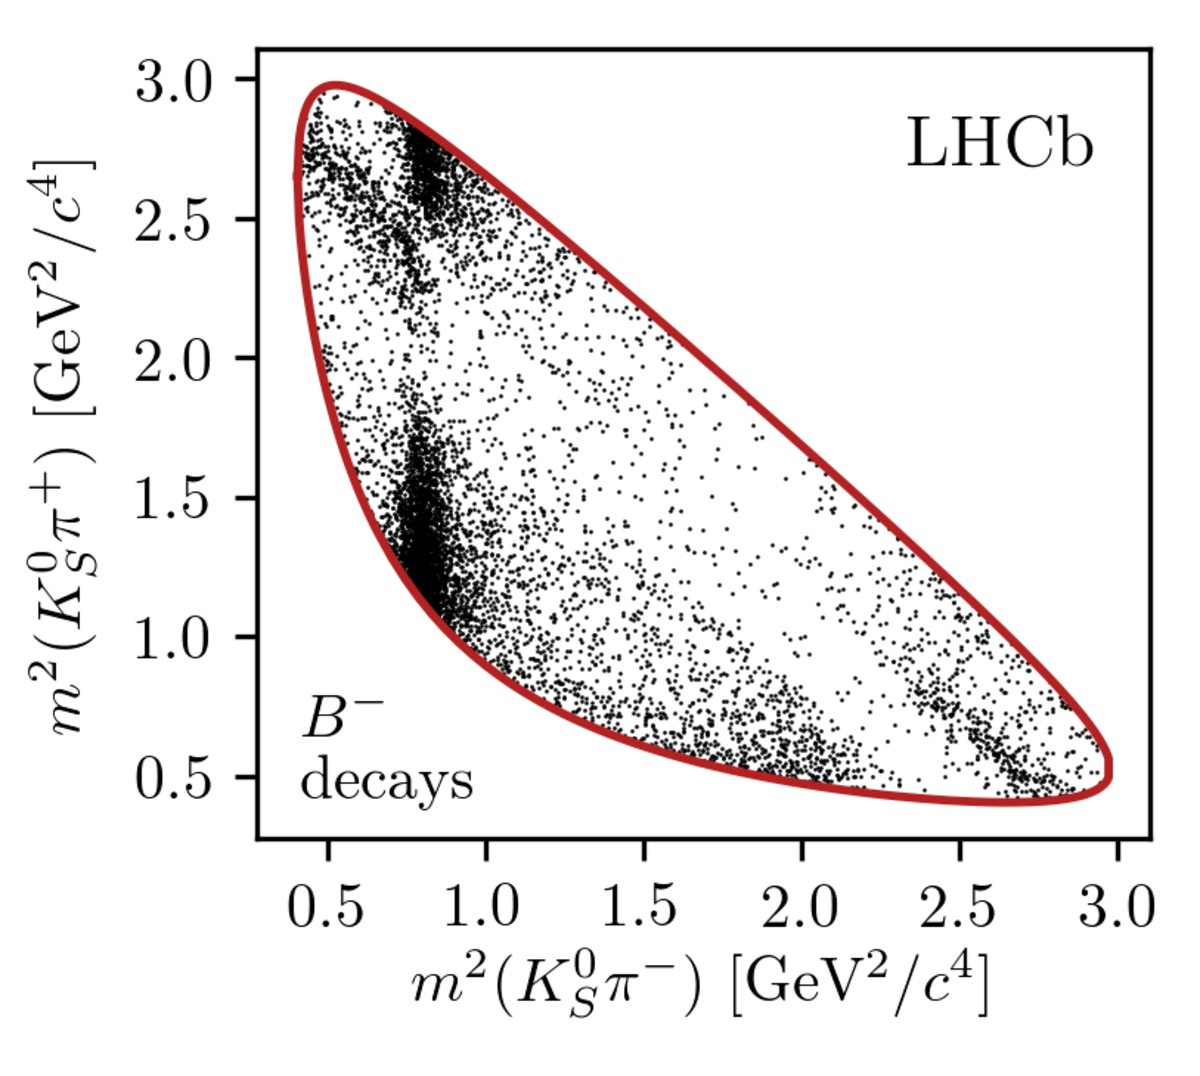
\includegraphics[width=1.0\textwidth]{Plots/KSpipi_Minus_Dalitz.png}};
        \node at(a.center)[draw, blue,line width=1pt,ellipse, minimum width=50pt, minimum height=20pt,rotate=0,yshift=-25pt,xshift=10pt]{};
      \end{tikzpicture}
      \vspace{-0.8cm}
      \caption*{$B^-\to[K_S^0\pi^+\pi^-]_DK^-$}
    \end{subfigure}%
    \begin{subfigure}{0.5\textwidth}
      \begin{tikzpicture}
        \node(a){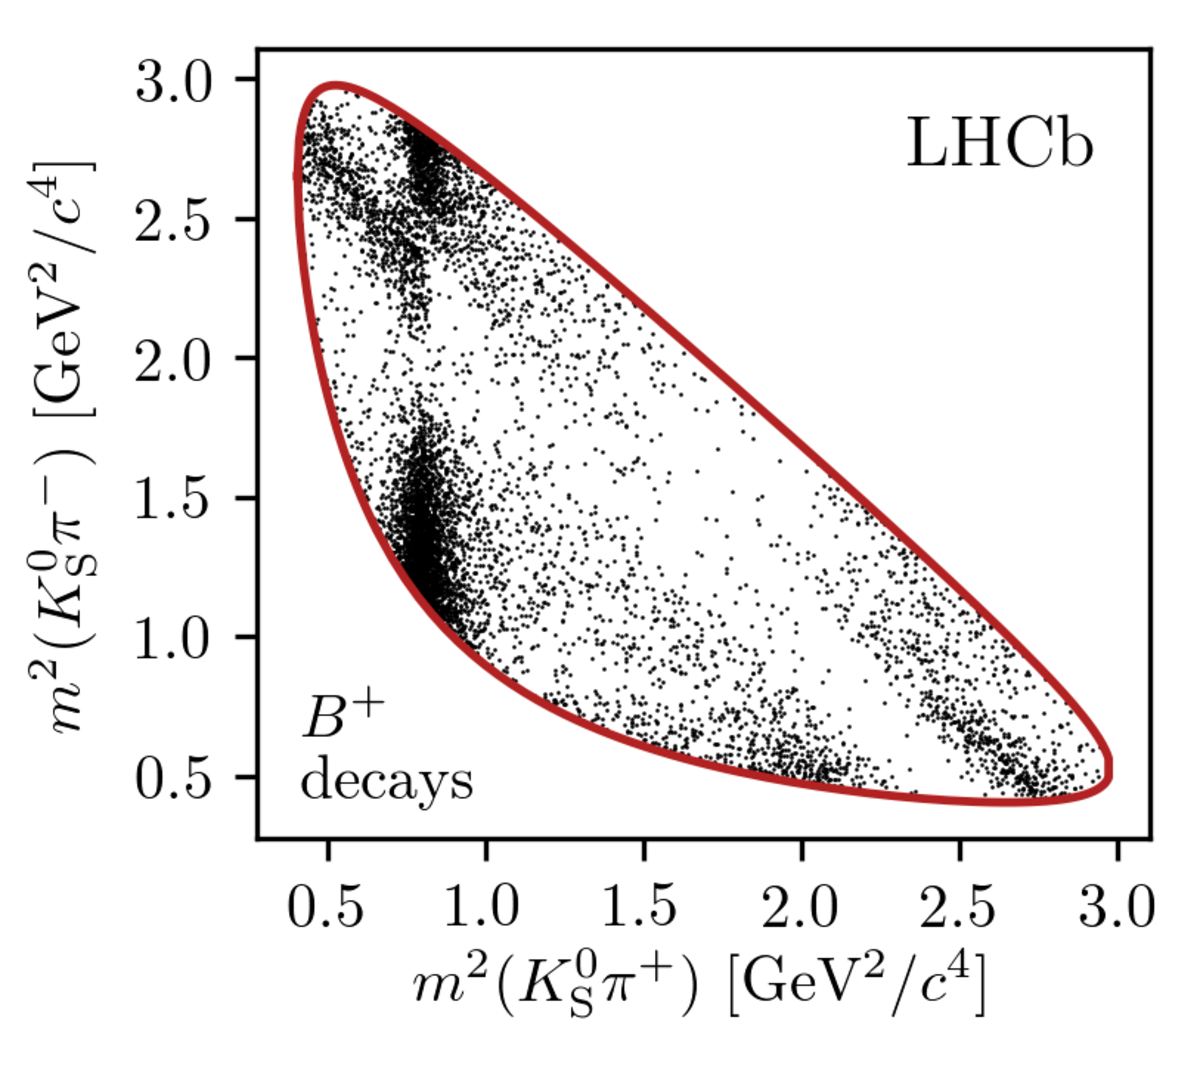
\includegraphics[width=1.0\textwidth]{Plots/KSpipi_Plus_Dalitz.png}};
        \node at(a.center)[draw, blue,line width=1pt,ellipse, minimum width=50pt, minimum height=20pt,rotate=0,yshift=-25pt,xshift=10pt]{};
      \end{tikzpicture}
      \vspace{-0.8cm}
      \caption*{$B^+\to[K_S^0\pi^+\pi^-]_DK^+$}
    \end{subfigure}
    \vspace{-0.3cm}
    \caption*{\tiny JHEP \textbf{02} (2021) 169}
  \end{figure}
  \vspace{-0.6cm}
  \begin{center}
    \Large Can you find the asymmetries?
  \end{center}
\end{frame}

\begin{frame}{Multi-body $D$ decays}
  \begin{figure}
    \begin{subfigure}{0.5\textwidth}
      \begin{tikzpicture}
        \node(a){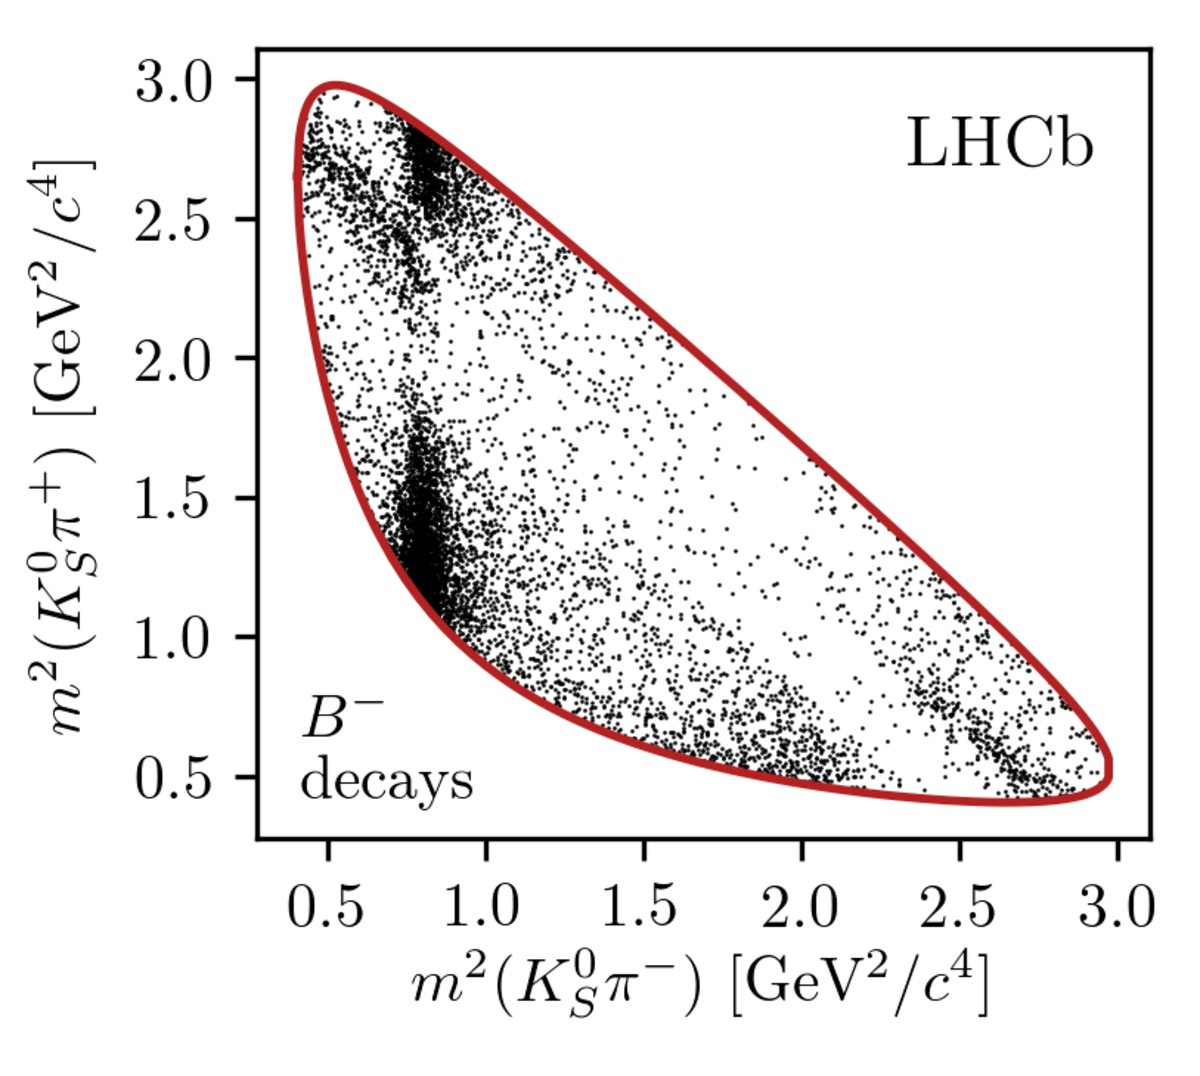
\includegraphics[width=1.0\textwidth]{Plots/KSpipi_Minus_Dalitz.png}};
        \node at(a.center)[draw, blue,line width=1pt,ellipse, minimum width=50pt, minimum height=20pt,rotate=0,yshift=-25pt,xshift=10pt]{};
        \node at(a.center)[draw, blue,line width=1pt,ellipse, minimum width=20pt, minimum height=40pt,rotate=0,yshift=40pt,xshift=-35pt]{};
      \end{tikzpicture}   
      \vspace{-0.8cm}
      \caption*{$B^-\to[K_S^0\pi^+\pi^-]_DK^-$}
    \end{subfigure}%
    \begin{subfigure}{0.5\textwidth}
      \begin{tikzpicture}
        \node(a){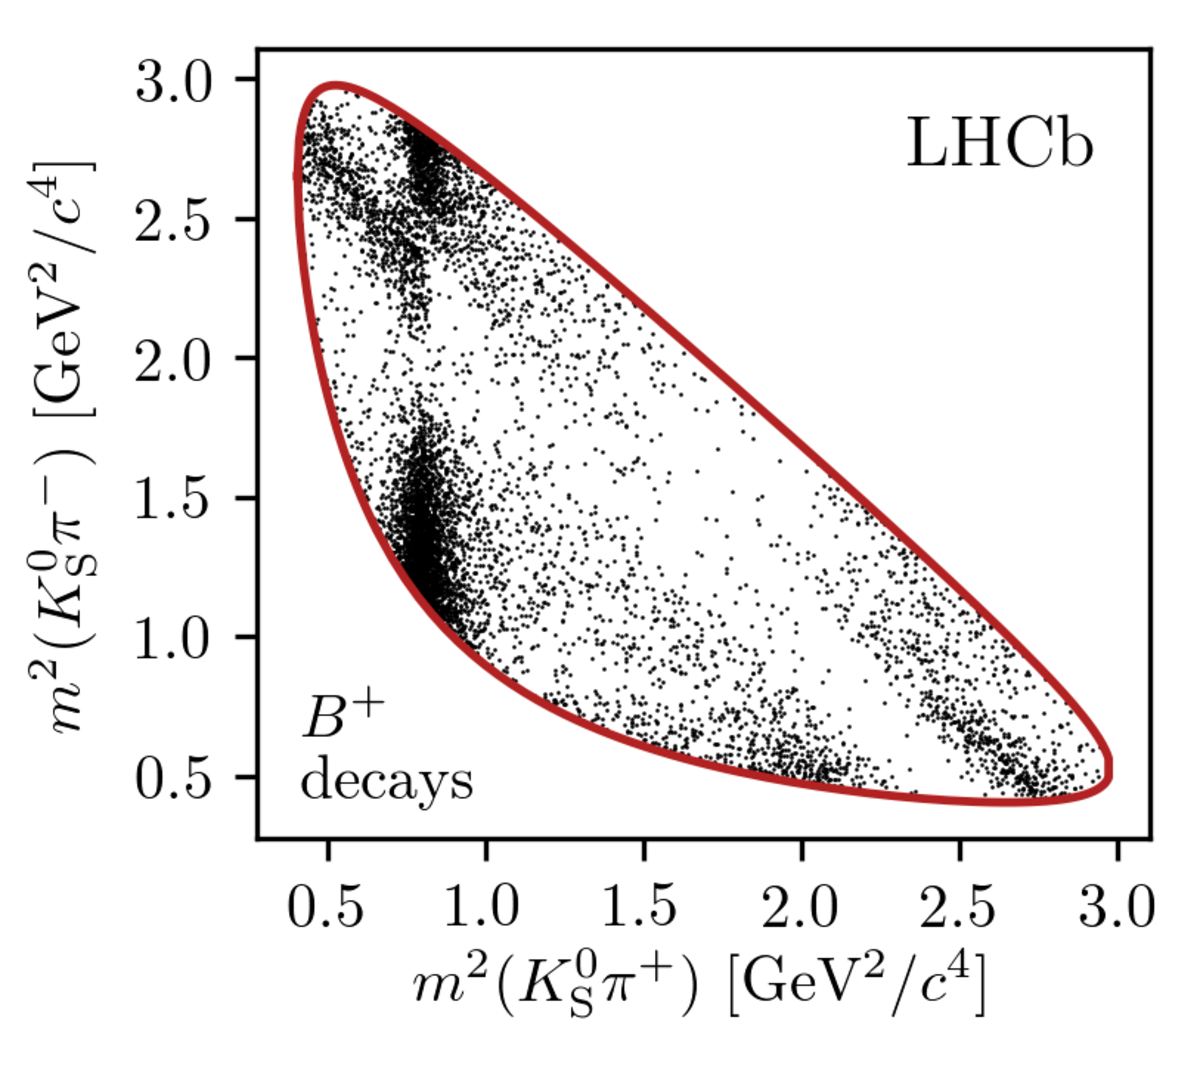
\includegraphics[width=1.0\textwidth]{Plots/KSpipi_Plus_Dalitz.png}};
        \node at(a.center)[draw, blue,line width=1pt,ellipse, minimum width=50pt, minimum height=20pt,rotate=0,yshift=-25pt,xshift=10pt]{};
        \node at(a.center)[draw, blue,line width=1pt,ellipse, minimum width=20pt, minimum height=40pt,rotate=0,yshift=40pt,xshift=-35pt]{};
      \end{tikzpicture}
      \vspace{-0.8cm}
      \caption*{$B^+\to[K_S^0\pi^+\pi^-]_DK^+$}
    \end{subfigure}
    \vspace{-0.3cm}
    \caption*{\tiny JHEP \textbf{02} (2021) 169}
  \end{figure}
  \vspace{-0.6cm}
  \begin{center}
    \Large Can you find the asymmetries?
  \end{center}
\end{frame}

\begin{frame}{Multi-body $D$ decays}
  \begin{itemize}
    \setlength\itemsep{0.5em}
    \item{Interpretation of $\gamma$ from the multi-body charm decays require external inputs of the charm strong-phase differences}
    \item{The three-body decays $D\to K_S^0h^+h^-$ have been studied extensively, using an optimised phase-space binning:}
    \begin{itemize}
      \item{CLEO \href{https://doi.org/10.1103/PhysRevD.82.112006}{Phys. Rev. \textbf{D82} (2010) 112006}}
      \item{BESIII \href{https://journals.aps.org/prd/abstract/10.1103/PhysRevD.101.112002}{Phys. Rev. \textbf{D101} (2020) 112002}}
    \end{itemize}
    \item{With charm inputs from CLEO and BESIII, the measurement of $\gamma$ becomes \underline{model independent}}
  \end{itemize}
  \begin{figure}
    \centering
    \begin{subfigure}{0.5\textwidth}
      \centering
      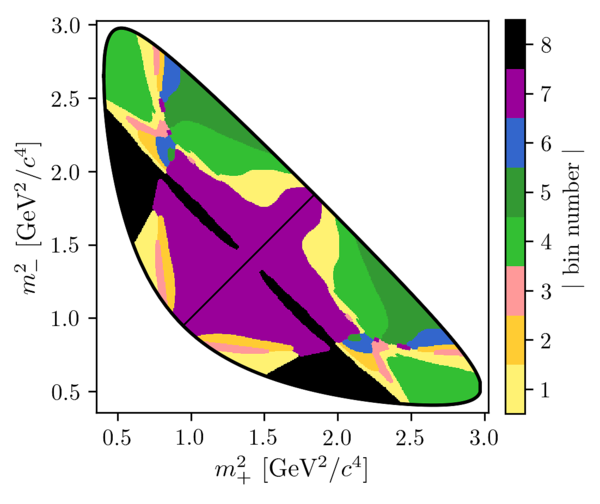
\includegraphics[height = 3.5cm]{Plots/KsPiPi_optimal.png}
      \vspace{-0.3cm}
      \caption*{$K_S^0\pi^+\pi^-$}
    \end{subfigure}%
    \begin{subfigure}{0.5\textwidth}
      \centering
      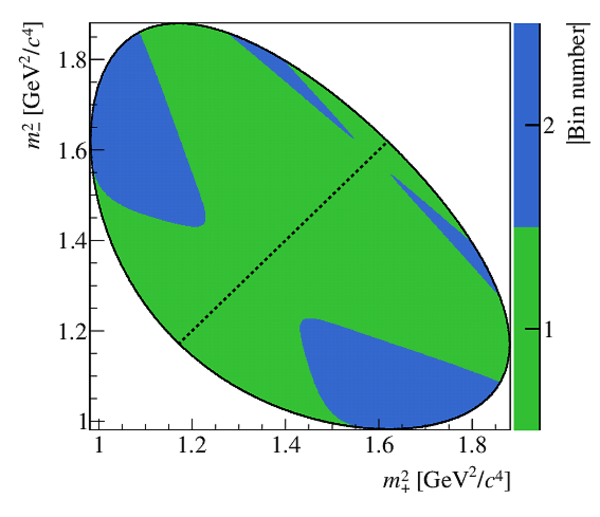
\includegraphics[height = 3.5cm]{Plots/KsKK_binning.png}
      \vspace{-0.3cm}
      \caption*{$K_S^0K^+K^-$}
    \end{subfigure}
    \vspace{-0.9cm}
    \caption*{\tiny JHEP \textbf{02} (2021) 169}
  \end{figure}
\end{frame}

\section{The LHCb \texorpdfstring{$\gamma$}{gamma} and charm combination}
\begin{frame}{The LHCb $\gamma$ and charm combination}
  \begin{center}
    {\huge The LHCb $\gamma$ and charm combination}\\~\\
    {\large Lots of beauty in charm!}
  \end{center}
\end{frame}

\begin{frame}{The LHCb $\gamma$ and charm combination}
  \begin{figure}
    \begin{overpic}[percent,width=0.7\textwidth]{Plots/gammacharm_lhcb_dhch_g_r_dk_2021.pdf}
    \end{overpic}
    \vspace{-0.5cm}
    \caption*{\tiny JHEP \textbf{12} (2021) 141}
  \end{figure}
  \begin{center}
    Currently, $\gamma$ measurements are dominated by $B^\pm\to Dh^\pm$
  \end{center}
\end{frame}

\begin{frame}{The LHCb $\gamma$ and charm combination}
  \begin{figure}
    \begin{overpic}[percent,width=0.7\textwidth]{Plots/gammacharm_lhcb_dhch_g_r_dk_2021.pdf}
      \put(5,-8){\vector(1.0,1.2){32}}
      \put(5,-8){\vector(1.0,0.6){64}}
    \end{overpic}
    \vspace{-0.5cm}
    \caption*{\tiny JHEP \textbf{12} (2021) 141}
  \end{figure}
  \begin{center}
    GLW+ADS: Narrow bands, but many degenerate solutions
  \end{center}
\end{frame}

\begin{frame}{The LHCb $\gamma$ and charm combination}
  \begin{figure}
    \begin{overpic}[percent,width=0.7\textwidth]{Plots/gammacharm_lhcb_dhch_g_r_dk_2021.pdf}
      \put(25,-8){\vector(1.0,1.7){20}}
    \end{overpic}
    \vspace{-0.5cm}
    \caption*{\tiny JHEP \textbf{12} (2021) 141}
  \end{figure}
  \begin{center}
    BPGGSZ: Wider, but unqiue solution
  \end{center}
\end{frame}

\begin{frame}{The LHCb $\gamma$ and charm combination}
  \begin{figure}
    \begin{overpic}[percent,width=0.7\textwidth]{Plots/gammacharm_lhcb_dhch_g_r_dk_2021.pdf}
    \end{overpic}
    \vspace{-0.5cm}
    \caption*{\tiny JHEP \textbf{12} (2021) 141}
  \end{figure}
  \begin{center}
    A combination of direct $\gamma$ measurements is necessary!
  \end{center}
\end{frame}

\begin{frame}{The LHCb $\gamma$ and charm combination}
  \begin{center}
    \Large Other $B$ decays are also interesting for $\gamma$ measurements:
  \end{center}
  \vspace{0.2cm}
  \begin{columns}
    \begin{column}{0.6\textwidth}
      \vspace{1.5cm}
      \begin{enumerate}
        \item{$B^\pm\to DK^\pm$}
        \item{$B^\pm\to D^{*0}K^\pm$}
        \item{$B^0\to DK^{*0}$}
        \item{$B_s^0\to D_s^-K^+$}
        \item[-]{And many more...}
      \end{enumerate}
      \vspace{1.5cm}
    \end{column}
    \begin{column}{0.4\textwidth}
    \end{column}
  \end{columns}
\end{frame}

\begin{frame}{The LHCb $\gamma$ and charm combination}
  \begin{center}
    \Large Other $B$ decays are also interesting for $\gamma$ measurements:
  \end{center}
  \vspace{0.2cm}
  \begin{columns}
    \begin{column}{0.6\textwidth}
      \vspace{1.5cm}
      \begin{enumerate}
        \item{$B^\pm\to DK^\pm$ $\leftarrow$ Golden mode}
        \item{$B^\pm\to D^{*0}K^\pm$}
        \item{$B^0\to DK^{*0}$}
        \item{$B_s^0\to D_s^-K^+$}
        \item[-]{And many more...}
      \end{enumerate}
      \vspace{1.5cm}
    \end{column}
    \begin{column}{0.4\textwidth}
    \end{column}
  \end{columns}
\end{frame}

\begin{frame}{The LHCb $\gamma$ and charm combination}
  \begin{center}
    \Large Other $B$ decays are also interesting for $\gamma$ measurements:
  \end{center}
  \vspace{0.2cm}
  \begin{columns}
    \begin{column}{0.6\textwidth}
      \vspace{1.5cm}
      \begin{enumerate}
        \item{$B^\pm\to DK^\pm$ $\leftarrow$ Golden mode}
        \item{$B^\pm\to D^{*0}K^\pm$ $\leftarrow$ New results!}
        \item{$B^0\to DK^{*0}$ $\leftarrow$ New results!}
        \item{$B_s^0\to D_s^-K^+$}
        \item[-]{And many more...}
      \end{enumerate}
      \vspace{1.5cm}
    \end{column}
    \begin{column}{0.4\textwidth}
    \end{column}
  \end{columns}
\end{frame}

\begin{frame}{The LHCb $\gamma$ and charm combination}
  \begin{center}
    \Large Other $B$ decays are also interesting for $\gamma$ measurements:
  \end{center}
  \vspace{0.2cm}
  \begin{columns}
    \begin{column}{0.6\textwidth}
      \vspace{1.5cm}
      \begin{enumerate}
        \item{$B^\pm\to DK^\pm$ $\leftarrow$ Golden mode}
        \item{$B^\pm\to D^{*0}K^\pm$ $\leftarrow$ New results!}
        \item{$B^0\to DK^{*0}$ $\leftarrow$ New results!}
        \item{$B_s^0\to D_s^-K^+$ $\leftarrow$ Not covered today}
        \item[-]{And many more...}
      \end{enumerate}
      \vspace{1.5cm}
    \end{column}
    \begin{column}{0.4\textwidth}
    \end{column}
  \end{columns}
\end{frame}

\begin{frame}{The LHCb $\gamma$ and charm combination}
  \begin{center}
    \Large Other $B$ decays are also interesting for $\gamma$ measurements:
  \end{center}
  \vspace{0.2cm}
  \begin{columns}
    \begin{column}{0.4\textwidth}
      \vspace{1.5cm}
      \begin{enumerate}
        \item{$B^\pm\to DK^\pm$}
        \item{$B^\pm\to D^{*0}K^\pm$}
        \item{$B^0\to DK^{*0}$}
        \item{$B_s^0\to D_s^-K^+$}
        \item[-]{And many more...}
      \end{enumerate}
      \vspace{1.5cm}
    \end{column}
    \begin{column}{0.6\textwidth}
      \begin{figure}
        \centering
        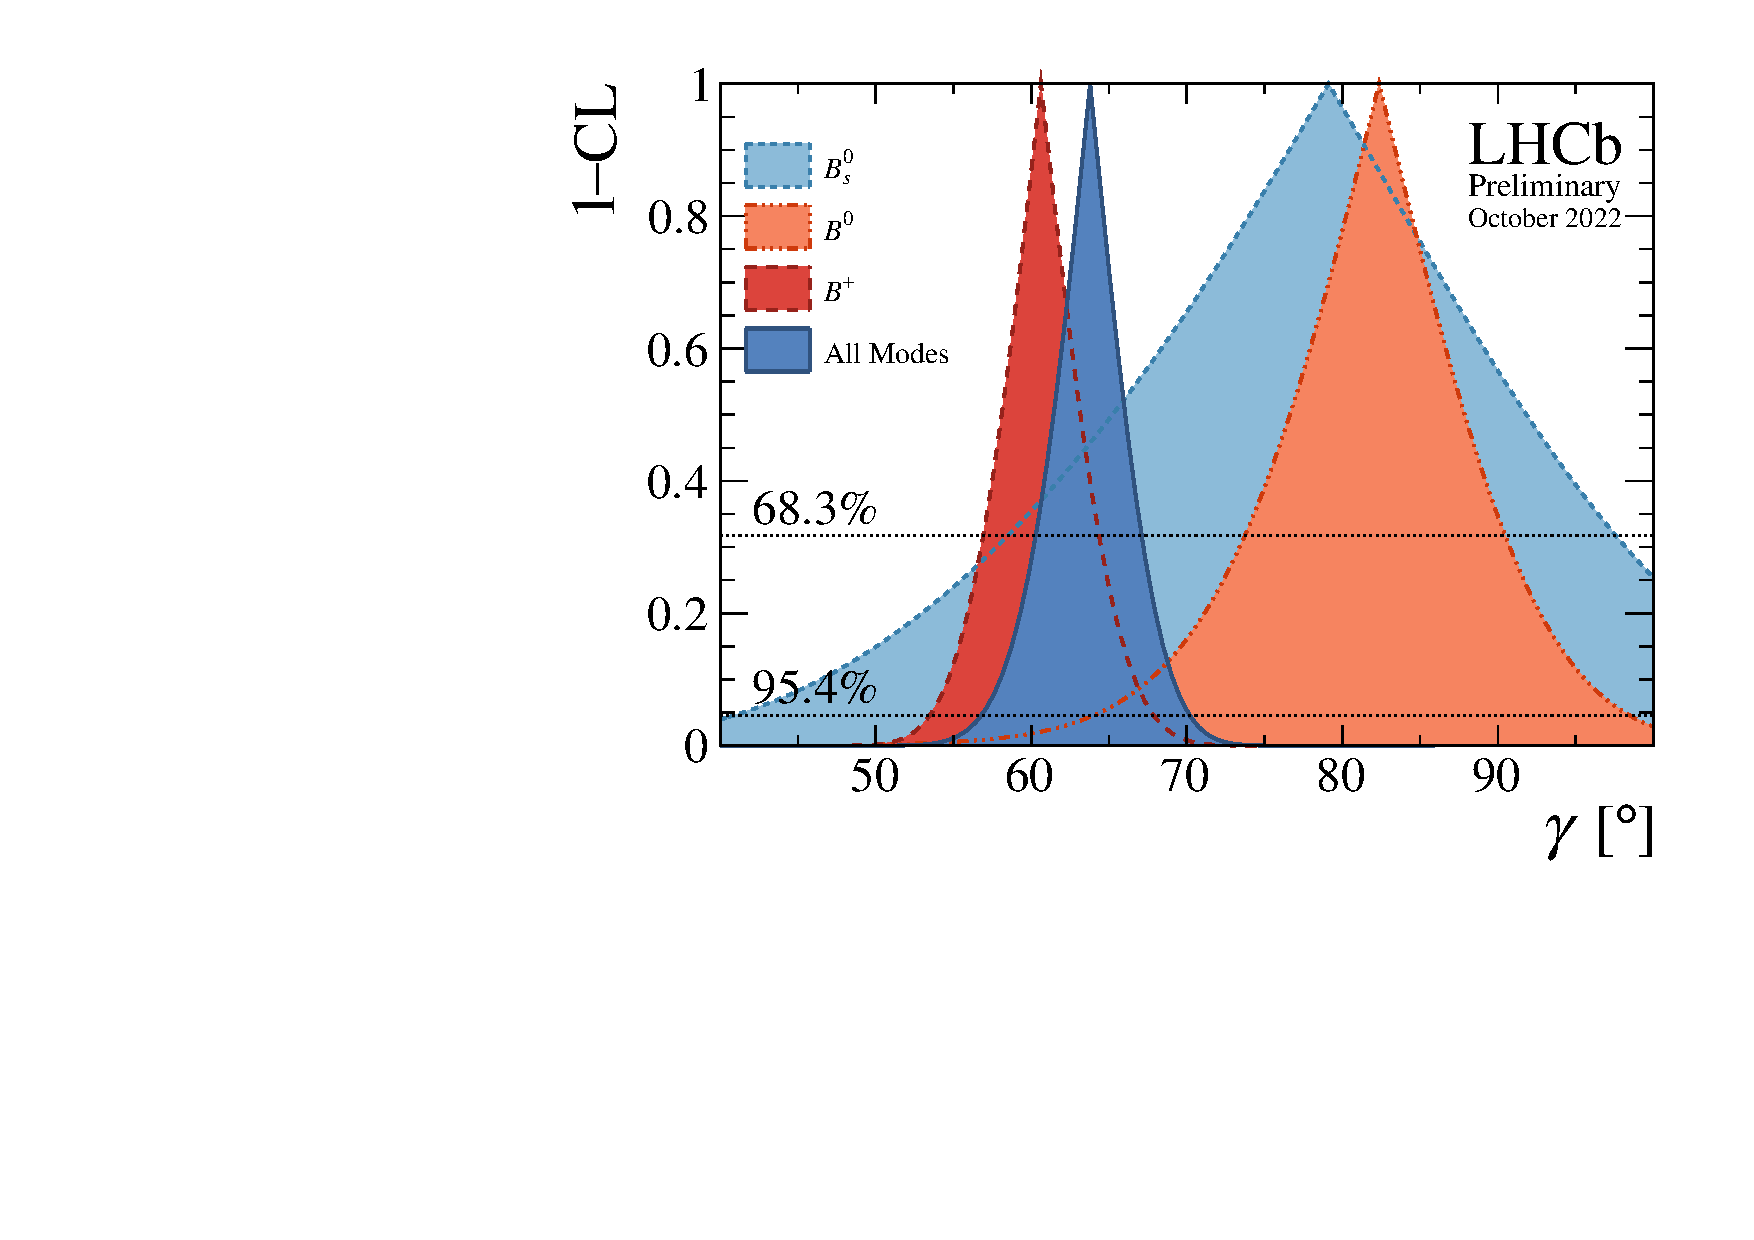
\includegraphics[width=0.8\textwidth]{Plots/gammacharm_lhcb_comp_flavour.pdf}
        \vspace{-0.5cm}
        \caption*{\tiny\href{https://lhcbproject.web.cern.ch/Publications/LHCbProjectPublic/LHCb-CONF-2022-003.html}{LHCb-CONF-2022-003}}
      \end{figure}
    \end{column}
  \end{columns}
\end{frame}

\begin{frame}{The LHCb $\gamma$ and charm combination}
  \begin{center}
    {\Large Our most precise knowledge of $\gamma$ comes from the combination of $\gamma$ and charm mixing parameters}\\~\\
  \end{center}
  \vspace{-0.5cm}
  \begin{figure}
    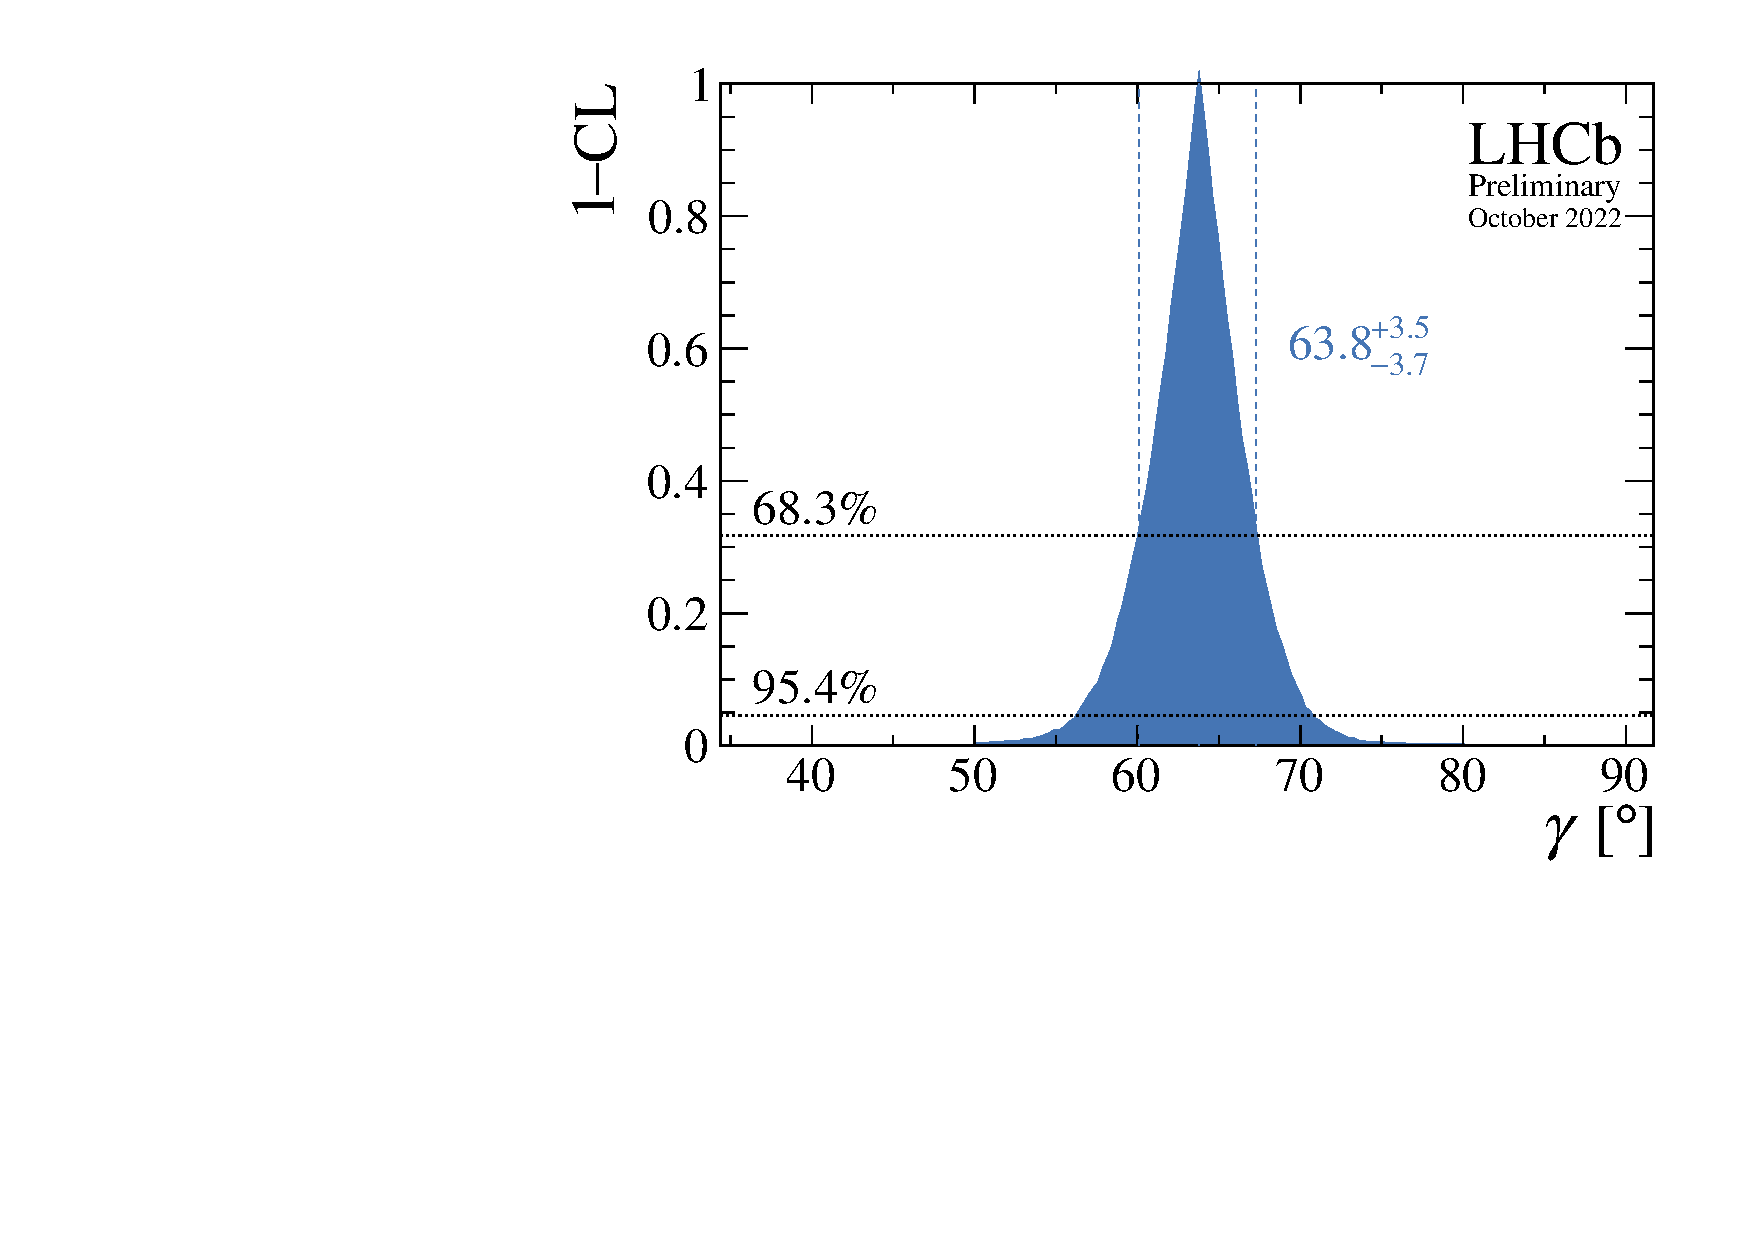
\includegraphics[height=5.0cm]{Plots/gammacharm_lhcb_gamma_only.pdf}
    \vspace{-0.5cm}
    \caption*{\tiny\href{https://lhcbproject.web.cern.ch/Publications/LHCbProjectPublic/LHCb-CONF-2022-003.html}{LHCb-CONF-2022-003}}
  \end{figure}
  \vspace{-0.5cm}
  \begin{center}
    This is the most precise determination of $\gamma$ by a single experiment!\\
    Charged $B^\pm$ modes dominate, but all measurements are consistent \phantom{$\delta_D^{K\pi}$}
  \end{center}
\end{frame}

\begin{frame}{The LHCb $\gamma$ and charm combination}
  \begin{center}
    {\Large Our most precise knowledge of $\gamma$ comes from the combination of $\gamma$ and charm mixing parameters}\\~\\
  \end{center}
  \vspace{-0.5cm}
  \begin{figure}
    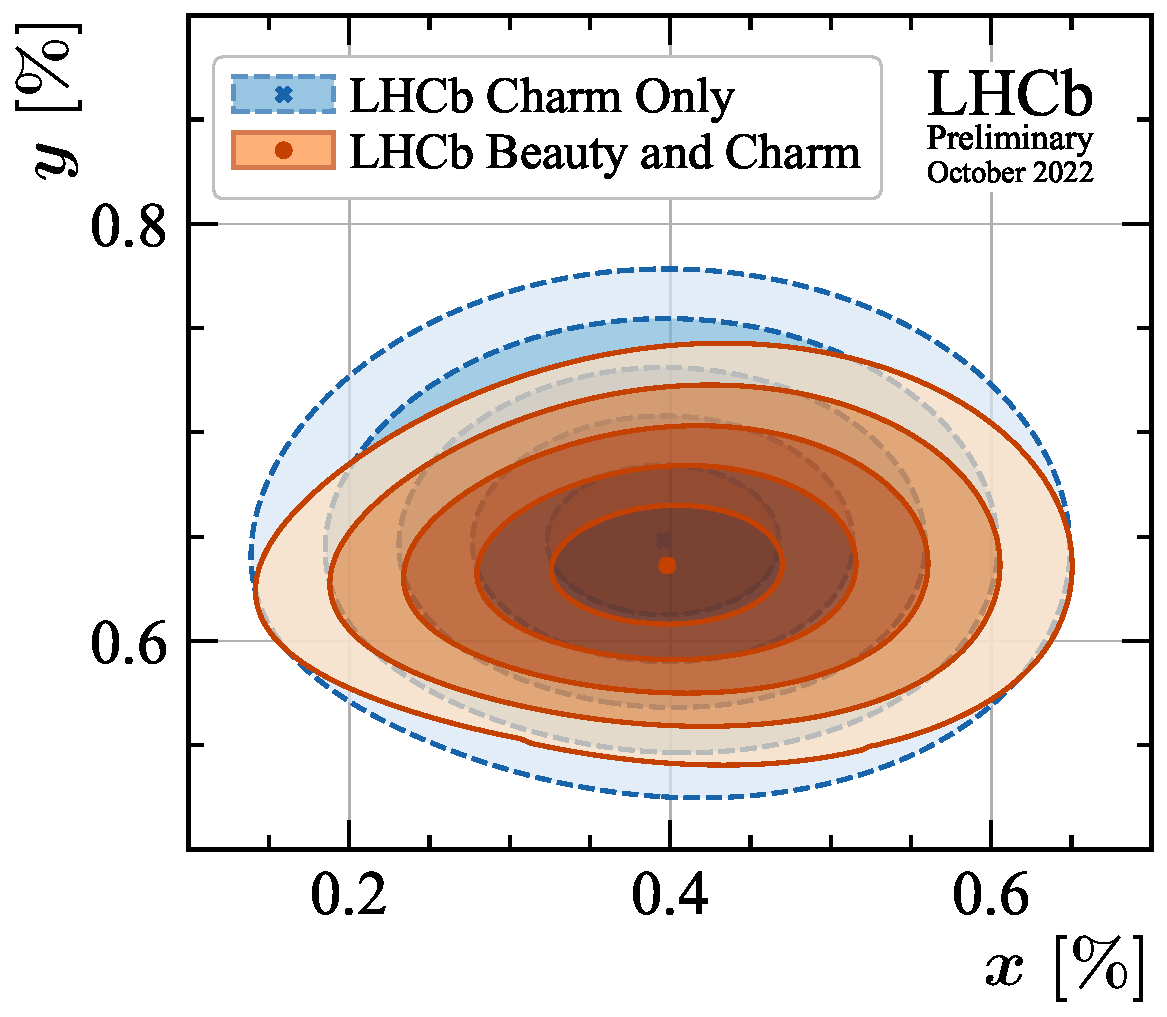
\includegraphics[height=5.0cm]{Plots/gammacharm_lhcb_xD_yD.pdf}
    \vspace{-0.5cm}
    \caption*{\tiny\href{https://lhcbproject.web.cern.ch/Publications/LHCbProjectPublic/LHCb-CONF-2022-003.html}{LHCb-CONF-2022-003}}
  \end{figure}
  \vspace{-0.5cm}
  \begin{center}
    Mixing effects to $\gamma$ measurements are approaching the statistical sensitivity\\
    Knowledge of $y$ is significantly improved through correlations with $\delta_D^{K\pi}$
  \end{center}
\end{frame}

\section{Neutral \texorpdfstring{$B$}{B} decays}
\begin{frame}{Neutral $B$ decays}
  \begin{center}
    {\huge Neutral $B$ decays} \\~\\
    {\large More interference with less statistics}
  \end{center}
\end{frame}

\begin{frame}{Neutral $B$ decays}
  \begin{center}
  {\Large Neutral $B$ decays are analysed with an identical strategy:}\\~\\
  {\large LHCb-PAPER-2023-009 (in preparation)\quad \colorbox{lime}{New results!}}\\
  \end{center}
  \vspace{0.5cm}
  \begin{figure}[H]
    \centering
    \begin{fmffile}{fgraph/fgraph_B02DKst_Kst2Kpi}
      \setlength{\unitlength}{0.7cm}
      \begin{fmfgraph*}(6,4)
        \fmfstraight
        \fmfleft{i1}
        \fmfv{decor.shape=circle,decor.filled=shaded,decor.size=0.2w,label=$B^0$,label.angle=180,label.dist=0.5cm}{i1}
        \fmfright{o1,o2,o3,g1,o4,o5}
        \fmflabel{$\pi^-$}{o1}
        \fmflabel{$\pi^+$}{o2}
        \fmflabel{$K_S^0$}{o3}
        \fmflabel{$\pi^-$}{o4}
        \fmflabel{$K^+$}{o5}
        \fmf{plain,tension=2.0}{i1,v1}
        \fmfv{decor.shape=circle,decor.filled=shaded,decor.size=0.15w,label=\small$K^*(892)^0$,label.angle=100,label.dist=1.7cm}{v1}
        \fmf{plain}{v1,o1}
        \fmf{plain}{v1,o2}
        \fmf{plain}{v1,o3}
        \fmf{dashes,tension=2.0}{i1,v2}
        \fmfv{decor.shape=circle,decor.filled=shaded,decor.size=0.15w,label=\footnotesize$D^0$,label.angle=-100,label.dist=1.6cm}{v2}
        \fmf{phantom}{v2,g1}
        \fmf{plain}{v2,o4}
        \fmf{plain}{v2,o5}
      \end{fmfgraph*}
    \end{fmffile}
  \end{figure}
  \vspace{0.5cm}
  \begin{center}
    {\Large $B^0\to(K_S^0h^+h^-)_D(K^+\pi^-)_{K^*}$}
  \end{center}
  \begin{center}
  {\large This results supersedes that of JHEP \textbf{08} (2016) 137}
  \end{center}
\end{frame}

\begin{frame}{Neutral $B$ decays}
  \begin{figure}
    \begin{subfigure}{0.45\textwidth}
      \centering
      \begin{overpic}[percent,height=4.0cm]{Plots/Kspp_LL_GF_B0toDKst.pdf}
        \put(58,32.7){\tiny Preliminary}
      \end{overpic}
      \caption*{LL}
    \end{subfigure}%
    \begin{subfigure}{0.45\textwidth}
      \centering
      \begin{overpic}[percent,height=4.0cm]{Plots/Kspp_DD_GF_B0toDKst.pdf}
        \put(58,32.7){\tiny Preliminary}
        \put(50,70){\vector(-1.0,-1.9){27}}
        \put(50,50){\vector(-1.0,-1.9){15}}
        \put(50,68){$B^0$ signal}
        \put(45,53){$B_s^0$ background}
      \end{overpic}
      \caption*{DD}
    \end{subfigure}
    \vspace{-0.5cm}
    \caption*{\tiny LHCb-PAPER-2023-009}
  \end{figure}
  \vspace{-0.5cm}
  \begin{itemize}
    \setlength\itemsep{0.5em}
    \item{Two separate selections of $K^0_S$:}
    \begin{itemize}
      \item{LL (long tracks): $K^0_S$ decays in the VELO}
      \item{DD (downstream tracks): $K^0_S$ decays downstream of the VELO}
    \end{itemize}
    \item{$B^0\to DK^{*0}$ candidates with $D\to K_S^0\pi^+\pi^-$ ($D\to K_S^0K^+K^-$):}
    \begin{itemize}
      \item{LL: $102 \pm 17$ ($12 \pm 6$)}
      \item{DD: $288 \pm 25$ ($32 \pm 8$)}
    \end{itemize}
  \end{itemize}
\end{frame}

\begin{frame}{Neutral $B$ decays}
  \begin{figure}
    \begin{subfigure}{0.5\textwidth}
      \begin{overpic}[percent,width=0.9\textwidth]{Plots/DP_pipi_Bzb_BtoDKst.pdf}
        \put(72,64){\tiny Preliminary}
      \end{overpic}
      \caption*{$\bar{B^0}$}
    \end{subfigure}%
    \begin{subfigure}{0.5\textwidth}
      \begin{overpic}[percent,width=0.9\textwidth]{Plots/DP_pipi_Bz_BtoDKst.pdf}
        \put(72,64){\tiny Preliminary}
      \end{overpic}
      \caption*{$B^0$}
    \end{subfigure}
    \caption*{$B^0\to[K_S^0\pi^+\pi^-]_DK^{*0}$ Dalitz plots}
  \end{figure}
  \vspace{-0.5cm}
  \begin{center}
    \Large Can you find the asymmetries?
  \end{center}
\end{frame}

\begin{frame}{Neutral $B$ decays}
  \begin{figure}
    \begin{overpic}[percent,height=5.0cm]{Plots/CPFitAsymmetry_B0toDKst.pdf}
      \put(34.5,39.5){\tiny Preliminary}
    \end{overpic}
    \vspace{-0.2cm}
    \caption*{\tiny LHCb-PAPER-2023-009}
  \end{figure}
  \begin{itemize}
    \setlength\itemsep{0.5em}
    \item{Non-zero bin asymmetries are seen:}
    \begin{itemize}
      \item{\underline{Large} asymmetries between $B^0$ ($\bar{B^0}$) bin pairs}
      \item{Very small CPV is expected in $B^0_s$ decays, and these are not looked for}
    \end{itemize}
    \item[]{\phantom{Asymmetries differ in size and magnitude across bins of phase space}}
  \end{itemize}
\end{frame}

\begin{frame}{Neutral $B$ decays}
  \begin{figure}
    \begin{overpic}[percent,height=5.0cm]{Plots/Asymmetry_110723_BtoDKst.pdf}
      \put(56.5,9.5){\tiny Preliminary}
    \end{overpic}
    \vspace{-0.2cm}
    \caption*{\tiny LHCb-PAPER-2023-009}
  \end{figure}
  \begin{itemize}
    \setlength\itemsep{0.5em}
    \item{Non-zero bin asymmetries are seen:}
    \begin{itemize}
      \item{\underline{Large} asymmetries between $B^0$ ($\bar{B^0}$) bin pairs}
      \item{Very small CPV is expected in $B^0_s$ decays, and these are not looked for}
    \end{itemize}
    \item{Asymmetries differ in size and magnitude across bins of phase space}
  \end{itemize}
\end{frame}

\begin{frame}{Neutral $B$ decays}
  \begin{figure}
    \centering
    \begin{subfigure}{0.45\textwidth}
      \centering
      \begin{overpic}[percent,height=4.0cm]{Plots/cp_contours_B0toDKst.pdf}
        \put(67,67.5){\tiny Preliminary}
      \end{overpic}
    \end{subfigure}%
    \begin{subfigure}{0.45\textwidth}
      \centering
      \begin{overpic}[percent,height=4.0cm]{Plots/B0ToDKStar_GGSZ_g_db_B0toDKst.pdf}
        \put(70.5,50){\tiny Preliminary}
      \end{overpic}
    \end{subfigure}
    \vspace{-0.2cm}
    \caption*{\tiny LHCb-PAPER-2023-009}
  \end{figure}
  \vspace{-0.5cm}
  \begin{itemize}
    \setlength\itemsep{0.5em}
    \item{Measured $C\!P$-violating observables:}
    \begin{center}
      $x_\pm\equiv r_{B^0}\cos(\delta_{B^0} \pm \gamma)$ and $y_\pm\equiv r_{B^0}\sin(\delta_{B^0} \pm \gamma)$
    \end{center}
    \item{Measured value of $\gamma$ is consistent with world average:}
    \begin{itemize}
      \item{$\gamma = (49 \pm 20)^\circ$}
      \item{$\delta_{B^0} = (236 \pm 19)^\circ$}
      \item{$r_{B^0} = 0.27 \pm 0.07$ $\leftarrow$ 3 times larger than the $B^\pm$ modes!}
    \end{itemize}
  \end{itemize}
\end{frame}






\section{\texorpdfstring{$B$}{B} decays to excited \texorpdfstring{$D^*$}{Dst} final states}
\begin{frame}{B decays to excited $D^*$ final states}
  \begin{center}
    {\huge B decays to excited $D^*$ final states}\\~\\
    {\large A measurement with neutral particles}
  \end{center}
\end{frame}

\begin{frame}{$B$ decays to excited $D^*$ final states}
  \begin{center}
  {\Large $B^-\to D^*K^-$ decays are also a powerful probe of CPV:}\\~\\
  {\large LHCb-PAPER-2023-012 (in preparation)\quad \colorbox{lime}{New results!}}
  \end{center}
  \vspace{0.5cm}
  \begin{figure}[H]
    \centering
    \begin{subfigure}{0.45\textwidth}
      \centering
      \begin{fmffile}{fgraph/fgraph_BtoDstK_pi0}
        \setlength{\unitlength}{0.7cm}
        \begin{fmfgraph*}(4,3)
          \fmfstraight
          \fmfleft{i1}
          \fmfv{decor.shape=circle,decor.filled=shaded,decor.size=0.2w,label=$B^-$,label.angle=180,label.dist=0.5cm}{i1}
          \fmfright{o1,o2,o3}
          \fmflabel{$K^-$}{o1}
          \fmflabel{$\pi^0$}{o2}
          \fmflabel{$D$}{o3}
          \fmf{dashes,tension=1.5}{i1,v1}
          \fmfv{decor.shape=circle,decor.filled=shaded,decor.size=0.15w,label=\small$D^*$,label.angle=100,label.dist=0.5cm}{v1}
          \fmf{plain}{v1,o2}
          \fmf{plain}{v1,o3}
          \fmf{plain}{i1,o1}
        \end{fmfgraph*}
      \end{fmffile}
      \vspace{0.5cm}
      \caption*{$B^-\to[D\pi^0]_{D^*}K^-$}
    \end{subfigure}%
    \begin{subfigure}{0.45\textwidth}
      \centering
      \begin{fmffile}{fgraph/fgraph_BtoDstK_gamma}
        \setlength{\unitlength}{0.7cm}
        \begin{fmfgraph*}(4,3)
          \fmfstraight
          \fmfleft{i1}
          \fmfv{decor.shape=circle,decor.filled=shaded,decor.size=0.2w,label=$B^-$,label.angle=180,label.dist=0.5cm}{i1}
          \fmfright{o1,o2,o3}
          \fmflabel{$K^-$}{o1}
          \fmflabel{$\gamma$}{o2}
          \fmflabel{$D$}{o3}
          \fmf{dashes,tension=1.5}{i1,v1}
          \fmfv{decor.shape=circle,decor.filled=shaded,decor.size=0.15w,label=\small$D^*$,label.angle=100,label.dist=0.5cm}{v1}
          \fmf{plain}{v1,o2}
          \fmf{plain}{v1,o3}
          \fmf{plain}{i1,o1}
        \end{fmfgraph*}
      \end{fmffile}
      \vspace{0.5cm}
      \caption*{$B^-\to[D\gamma]_{D^*}K^-$}
    \end{subfigure}
  \end{figure}
  \vspace{-0.5cm}
  \begin{columns}
    \begin{column}{0.5\textwidth}
      \begin{center}
        $\mathcal{A}(D^0) + r_Be^{i(\delta_B - \gamma)}\mathcal{A}(\bar{D^0})$
      \end{center}
    \end{column}
    \begin{column}{0.5\textwidth}
      \begin{center}
        $\mathcal{A}(D^0) - r_Be^{i(\delta_B - \gamma)}\mathcal{A}(\bar{D^0})$
      \end{center}
    \end{column}
  \end{columns}
  \begin{center}
    The relative sign swap, due to the phase difference of $\pi$ between $\pi^0$ and $\gamma$,  results in \underline{opposite} $C\!P$ asymmetries between $D^*\to D\pi^0$ and $D^*\to D\gamma$
  \end{center}
\end{frame}

\begin{frame}{$B$ decays to excited $D^*$ final states}
  \begin{figure}
    \centering
    \begin{subfigure}{0.5\textwidth}
      \centering
      \begin{overpic}[percent,width=0.8\textwidth]{Plots/massfitPage_canvas_pi0_d2kspipi_b2dk_LL_merge_BtoDstK.pdf}
        \put(59,82){\tiny Preliminary}
        \put(36,48){\vector(-1.0,1.9){14}}
        \put(36,48){\vector(-1.0,-1.5){14}}
        \put(37,47.5){\scriptsize Signal peak}
      \end{overpic}
      \caption*{$D^*\to D\pi^0$}
    \end{subfigure}%
    \begin{subfigure}{0.5\textwidth}
      \centering
      \begin{overpic}[percent,width=0.8\textwidth]{Plots/massfitPage_canvas_gamma_d2kspipi_b2dk_LL_merge_BtoDstK.pdf}
        \put(59,82){\tiny Preliminary}
        \put(26,49){\vector(1.0,30.0){0.8}}
        \put(26,49){\vector(1.0,-0.8){31}}
        \put(0,49){\scriptsize Signal peak}
      \end{overpic}
      \caption{$D^*\to D\gamma$}
    \end{subfigure}
    \vspace{-0.5cm}
    \caption*{\tiny LHCb-PAPER-2023-012}
  \end{figure}
  \vspace{-0.5cm}
  \begin{center}
    A 2D fit is necessary to separate signal from background
  \end{center}
\end{frame}

\begin{frame}{$B$ decays to excited $D^*$ final states}
  \begin{figure}
    \begin{overpic}[percent,height=5.0cm]{Plots/histCPVnewd2kspipib2dk_BtoDstK.png}
      \put(57.5,32){\tiny Preliminary}
    \end{overpic}
    \vspace{-0.4cm}
    \caption*{\tiny LHCb-PAPER-2023-012}
  \end{figure}
  \vspace{-0.5cm}
  \begin{itemize}
    \setlength\itemsep{0.5em}
    \item{Good agreement between individual bin asymmetries and the combined $C\!P$ fit}
    \item{Bin asymmetries between $D^*\to D\pi^0$ and $D^*\to D\gamma$ are generally \underline{opposite} in sign}
  \end{itemize}
\end{frame}

\begin{frame}{$B$ decays to excited $D^*$ final states}
  \begin{figure}
    \centering
    \begin{subfigure}{0.5\textwidth}
      \centering
      \begin{overpic}[percent,height=5.0cm]{Plots/xyfinalres_BtoDstK.pdf}
        \put(27,69){\tiny Preliminary}
      \end{overpic}
    \end{subfigure}%
    \begin{subfigure}{0.5\textwidth}
      \centering
      \begin{overpic}[percent,height=4.3cm]{Plots/cartesian_cartesian1_g_r_dk_BtoDstK.pdf}
        \put(72,54){\tiny Preliminary}
      \end{overpic}
    \end{subfigure}
    \vspace{-0.8cm}
    \caption*{\tiny LHCb-PAPER-2023-012}
  \end{figure}
  \vspace{-0.7cm}
  \begin{center}
    These results provide strong constraints on $\gamma$:
  \end{center}
  \vspace{-0.2cm}
  \begin{itemize}
  \item{$\gamma = (69 \pm 14)^\circ$}
  \item{$\delta_B^{D^*K} = (311 \pm 15)^\circ$}
  \item{$r_B^{D^*K} = 0.15 \pm 0.03$}
  \end{itemize}
\end{frame}

\section{Binned four-body decay: \texorpdfstring{$D^0\to K^+K^-\pi^+\pi^-$}{DtoKKpipi}}
\begin{frame}{Binned four-body decay: $D^0\to K^+K^-\pi^+\pi^-$}
  \begin{center}
    {\huge Binned four-body decay: $D^0\to K^+K^-\pi^+\pi^-$}\\~\\
    {\large A journey through five dimensions}
  \end{center}
\end{frame}

\begin{frame}{Binned four-body decay: $D^0\to K^+K^-\pi^+\pi^-$}
  \begin{center}
    {\large Back to $D^0\to K_S^0h^+h^-$ binning schemes, visualised on a Dalitz plot:}
  \end{center}
  \vspace{-0.3cm}
  \begin{figure}
    \begin{subfigure}{0.45\textwidth}
      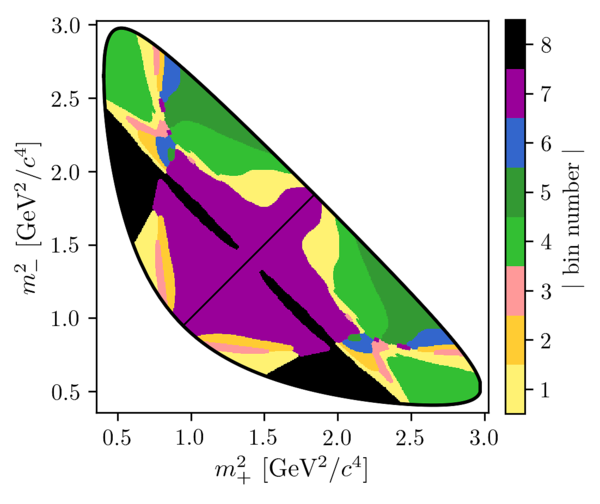
\includegraphics[height = 4cm]{Plots/KsPiPi_optimal.png}
      \vspace{-0.3cm}
      \caption*{$K_S^0\pi^+\pi^-$}
    \end{subfigure}%
    \begin{subfigure}{0.45\textwidth}
      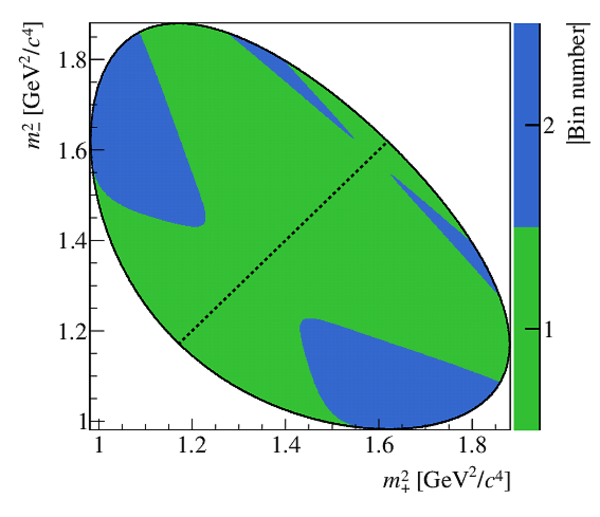
\includegraphics[height = 4cm]{Plots/KsKK_binning.png}
      \vspace{-0.3cm}
      \caption*{$K_S^0K^+K^-$}
    \end{subfigure}
  \end{figure}
  \begin{itemize}
    \setlength\itemsep{0.5em}
    \item{Bin boundaries are optimised for sensitivity to $\gamma$ by CLEO}
    \item{We would like to do this for $D^0\to K^+K^-\pi^+\pi^-$...}
    \item[]{\phantom{... but the four-body phase space is five-dimensional!}}
  \end{itemize}
\end{frame}

\begin{frame}{Binned four-body decay: $D^0\to K^+K^-\pi^+\pi^-$}
  \begin{center}
    {\large Back to $D^0\to K_S^0h^+h^-$ binning schemes, visualised on a Dalitz plot:}
  \end{center}
  \vspace{-0.3cm}
  \begin{figure}
    \begin{subfigure}{0.45\textwidth}
      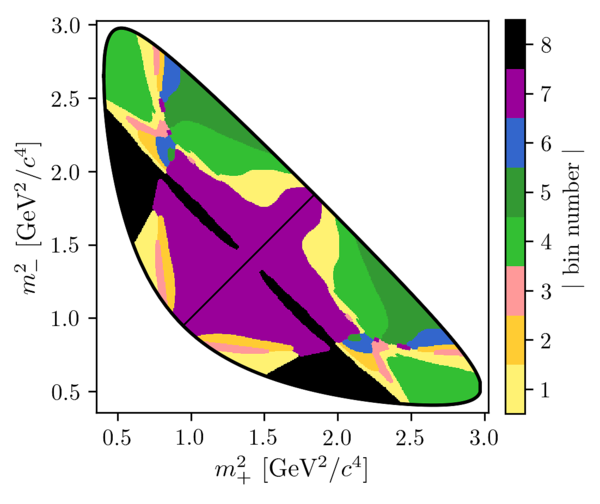
\includegraphics[height = 4cm]{Plots/KsPiPi_optimal.png}
      \vspace{-0.3cm}
      \caption*{$K_S^0\pi^+\pi^-$}
    \end{subfigure}%
    \begin{subfigure}{0.45\textwidth}
      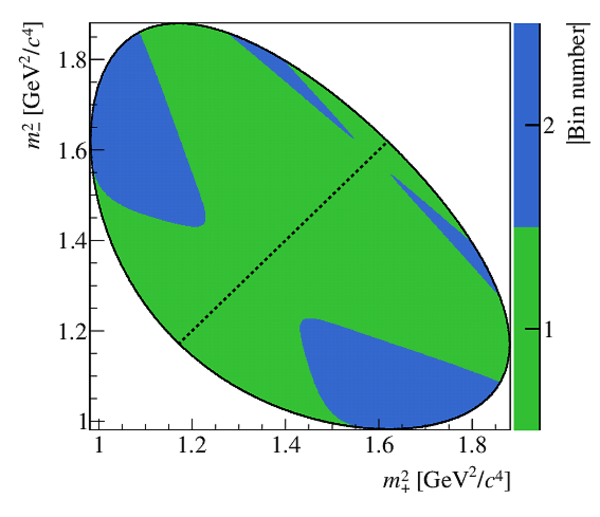
\includegraphics[height = 4cm]{Plots/KsKK_binning.png}
      \vspace{-0.3cm}
      \caption*{$K_S^0K^+K^-$}
    \end{subfigure}
  \end{figure}
  \begin{itemize}
    \setlength\itemsep{0.5em}
    \item{Bin boundaries are optimised for sensitivity to $\gamma$ by CLEO}
    \item{We would like to do this for $D^0\to K^+K^-\pi^+\pi^-$...}
    \item{... but the four-body phase space is five-dimensional!}
  \end{itemize}
\end{frame}

\begin{frame}{Binned four-body decay: $D^0\to K^+K^-\pi^+\pi^-$}
  \begin{center}
    \Large But how do we navigate through a 5D space?
  \end{center}
  \vspace{-0.5cm}
  \begin{figure}
    \centering
    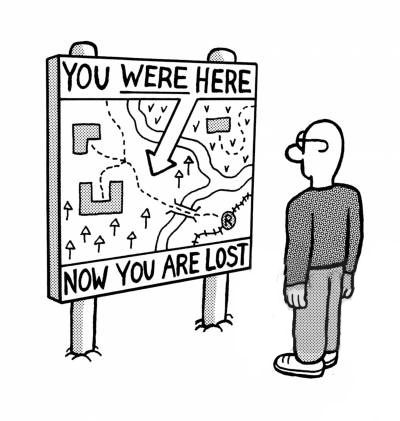
\includegraphics[width = 0.35\textwidth]{Plots/TravelLost.jpeg}
  \end{figure}
  \vspace{-0.7cm}
  \begin{center}
    \Large Use an amplitude model! JHEP \textbf{02} (2019) 126\\~\\
    \large Ultimately, the charm strong-phase differences will be measured directly at BESIII, and the $\gamma$ measurement will be \underline{model independent}
  \end{center}
\end{frame}

\begin{frame}{Binned four-body decay: $D^0\to K^+K^-\pi^+\pi^-$}
  \vspace{0.0cm}
  {\Large A binning scheme must satisfy the following:}
  \begin{itemize}
    \item{Minimal dilution of strong phases when integrating over bins}
    \item{Enhance interference between $B^\pm\to D^0K^\pm$ and $B^\pm\to\bar{D^0}K^\pm$}
  \end{itemize}
  \vspace{0.4cm}
  {\Large How to bin a 5-dimensional phase space?}
  \begin{enumerate}
    \item{For each $B^\pm$ candidate, use the amplitude model to calculate}
  \end{enumerate}
  \begin{center}
    {\Large $\frac{\mathcal{A}(D^0)}{\mathcal{A}(\bar{D^0})} = r_De^{i\delta_D}$}
  \end{center}
  \begin{enumerate}
    \setcounter{enumi}{1}
    \setlength\itemsep{0.5em}
    \item{Split $\delta_D$ into uniformly spaced bins}
    \item{Use the symmetry line $r_D = 1$ to separate bin $+i$ from $-i$}
    \item{Optimise the binning scheme by adjusting the bin boundaries in $\delta_D$}
  \end{enumerate}
\end{frame}

\begin{frame}{Binning scheme}
  \begin{figure}
    \centering
    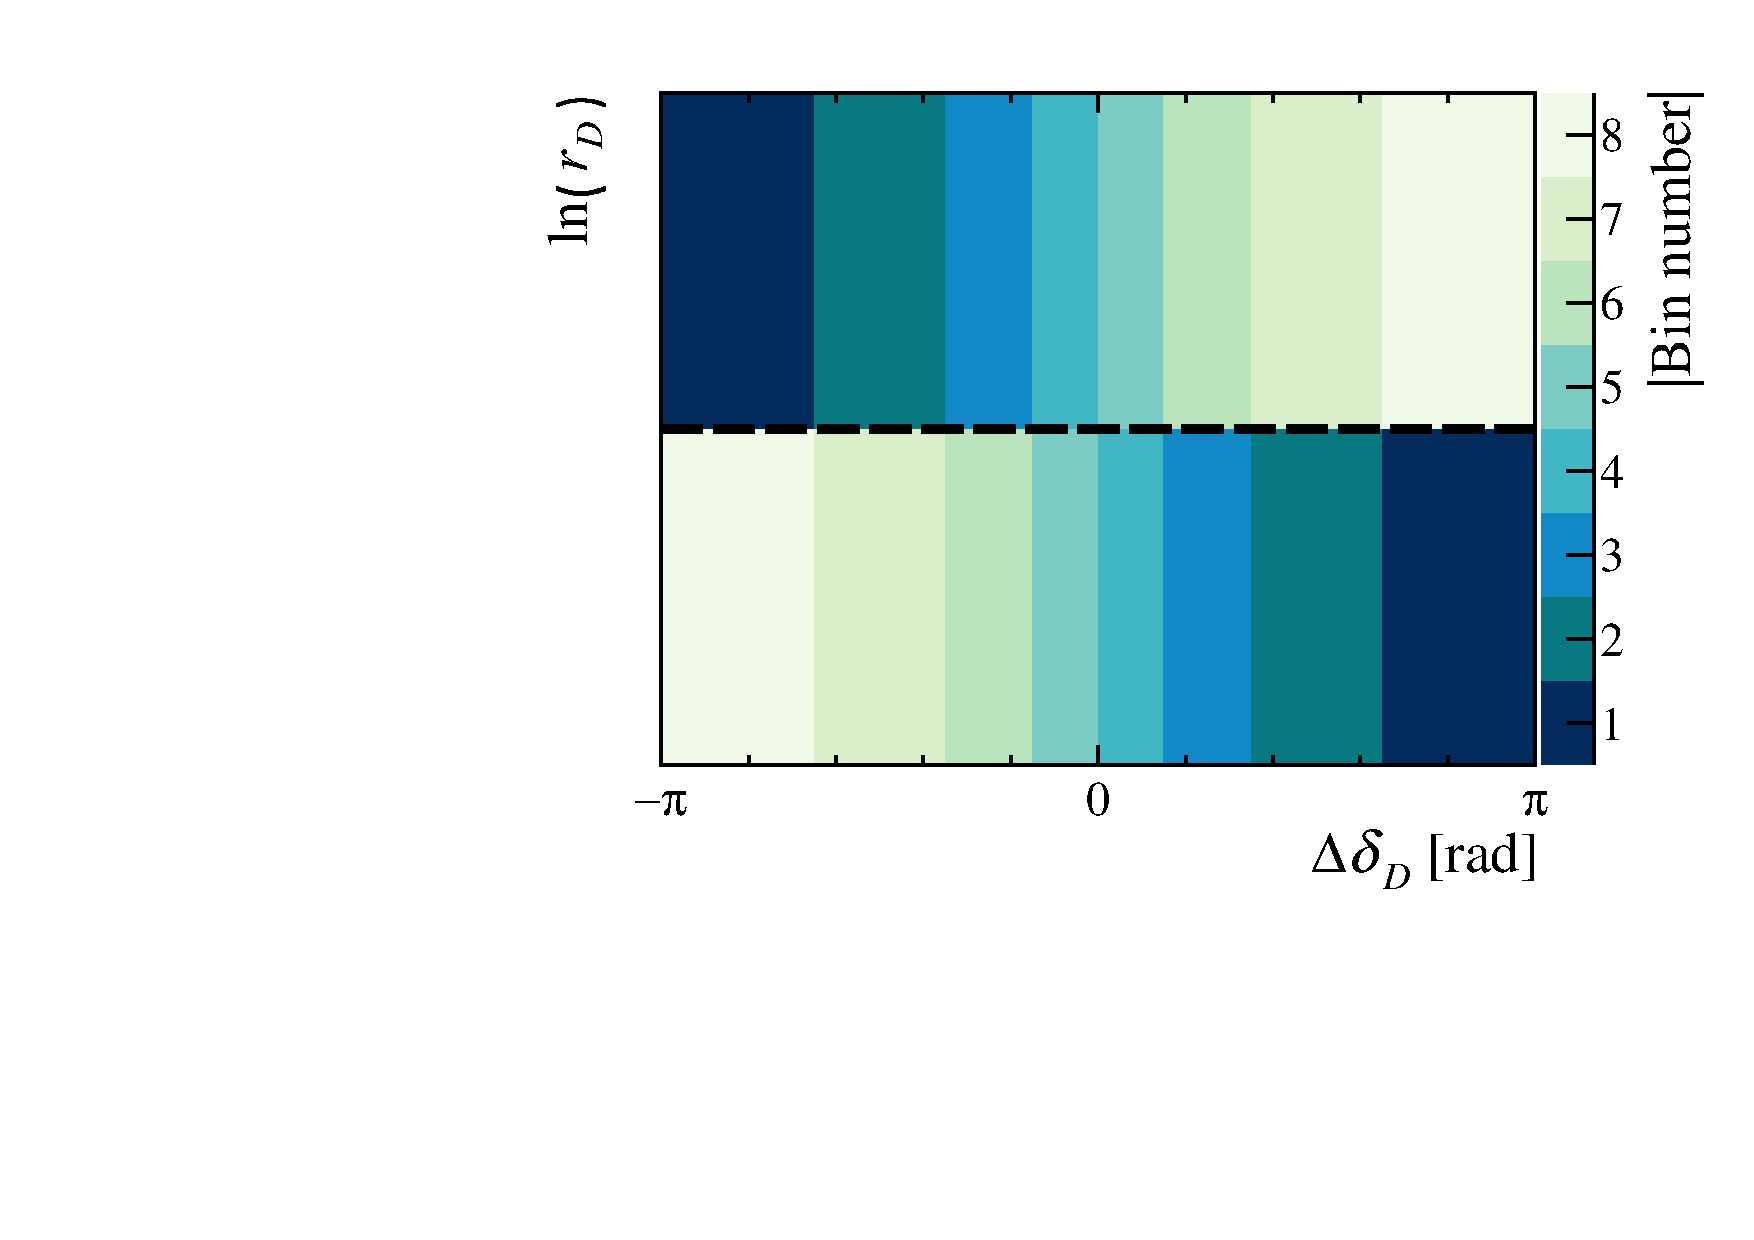
\includegraphics[width = 0.7\textwidth]{Plots/BinningSchemePlot_8Bins.pdf}
  \end{figure}
  \vspace{-1.0cm}
  \begin{center}
    $Q = 0.90$ \\
    Bins $i < 0$ on top, $i > 0$ below
  \end{center}
\end{frame}

\begin{frame}{Phase-space binned $B^\pm\to[K^+K^-\pi^+\pi^-]_DK^\pm$}
  \begin{center}
    {\large Fully charged final state $\implies$ Highly suitable for LHCb}
  \end{center}
  \begin{figure}
    \centering
    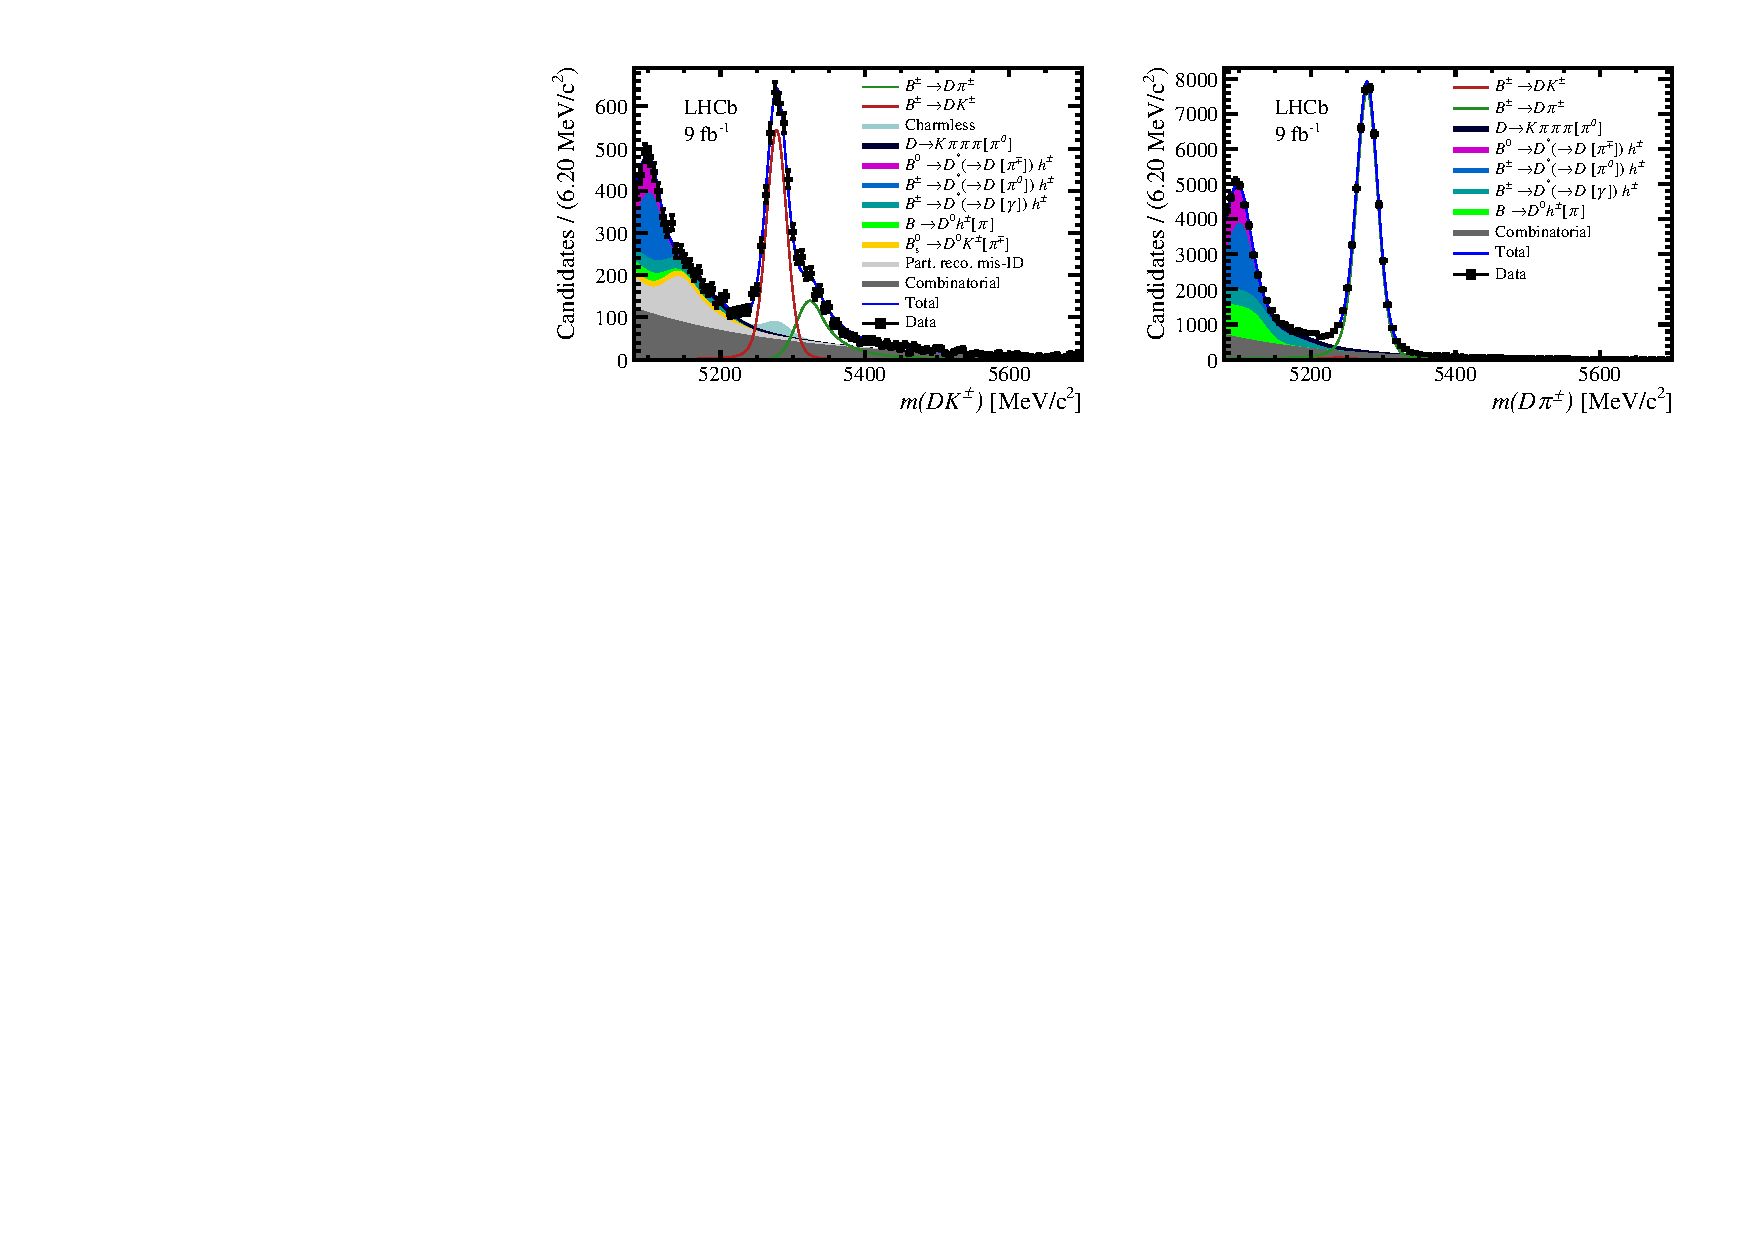
\includegraphics[width = 1.0\textwidth,trim={0 0 0 0},clip=true]{Plots/d2kkpipi_fiveL_allDP.pdf}
    \caption*{\tiny Eur. Phys. J. C \textbf{83}, 547 (2023)}
  \end{figure}
  \vspace{-0.5cm}
  \begin{itemize}
    \item{$B^\pm\to[K^+K^-\pi^+\pi^-]_Dh^\pm$ signal yield:}
    \begin{itemize}
      \item{$B^\pm\to DK^\pm$: $3026 \pm 38$}
      \item{$B^\pm\to D\pi^\pm$: $44349 \pm 218$}
    \end{itemize}
  \end{itemize}
\end{frame}

\begin{frame}{Phase-space binned $B^\pm\to[K^+K^-\pi^+\pi^-]_DK^\pm$}
  \begin{figure}
    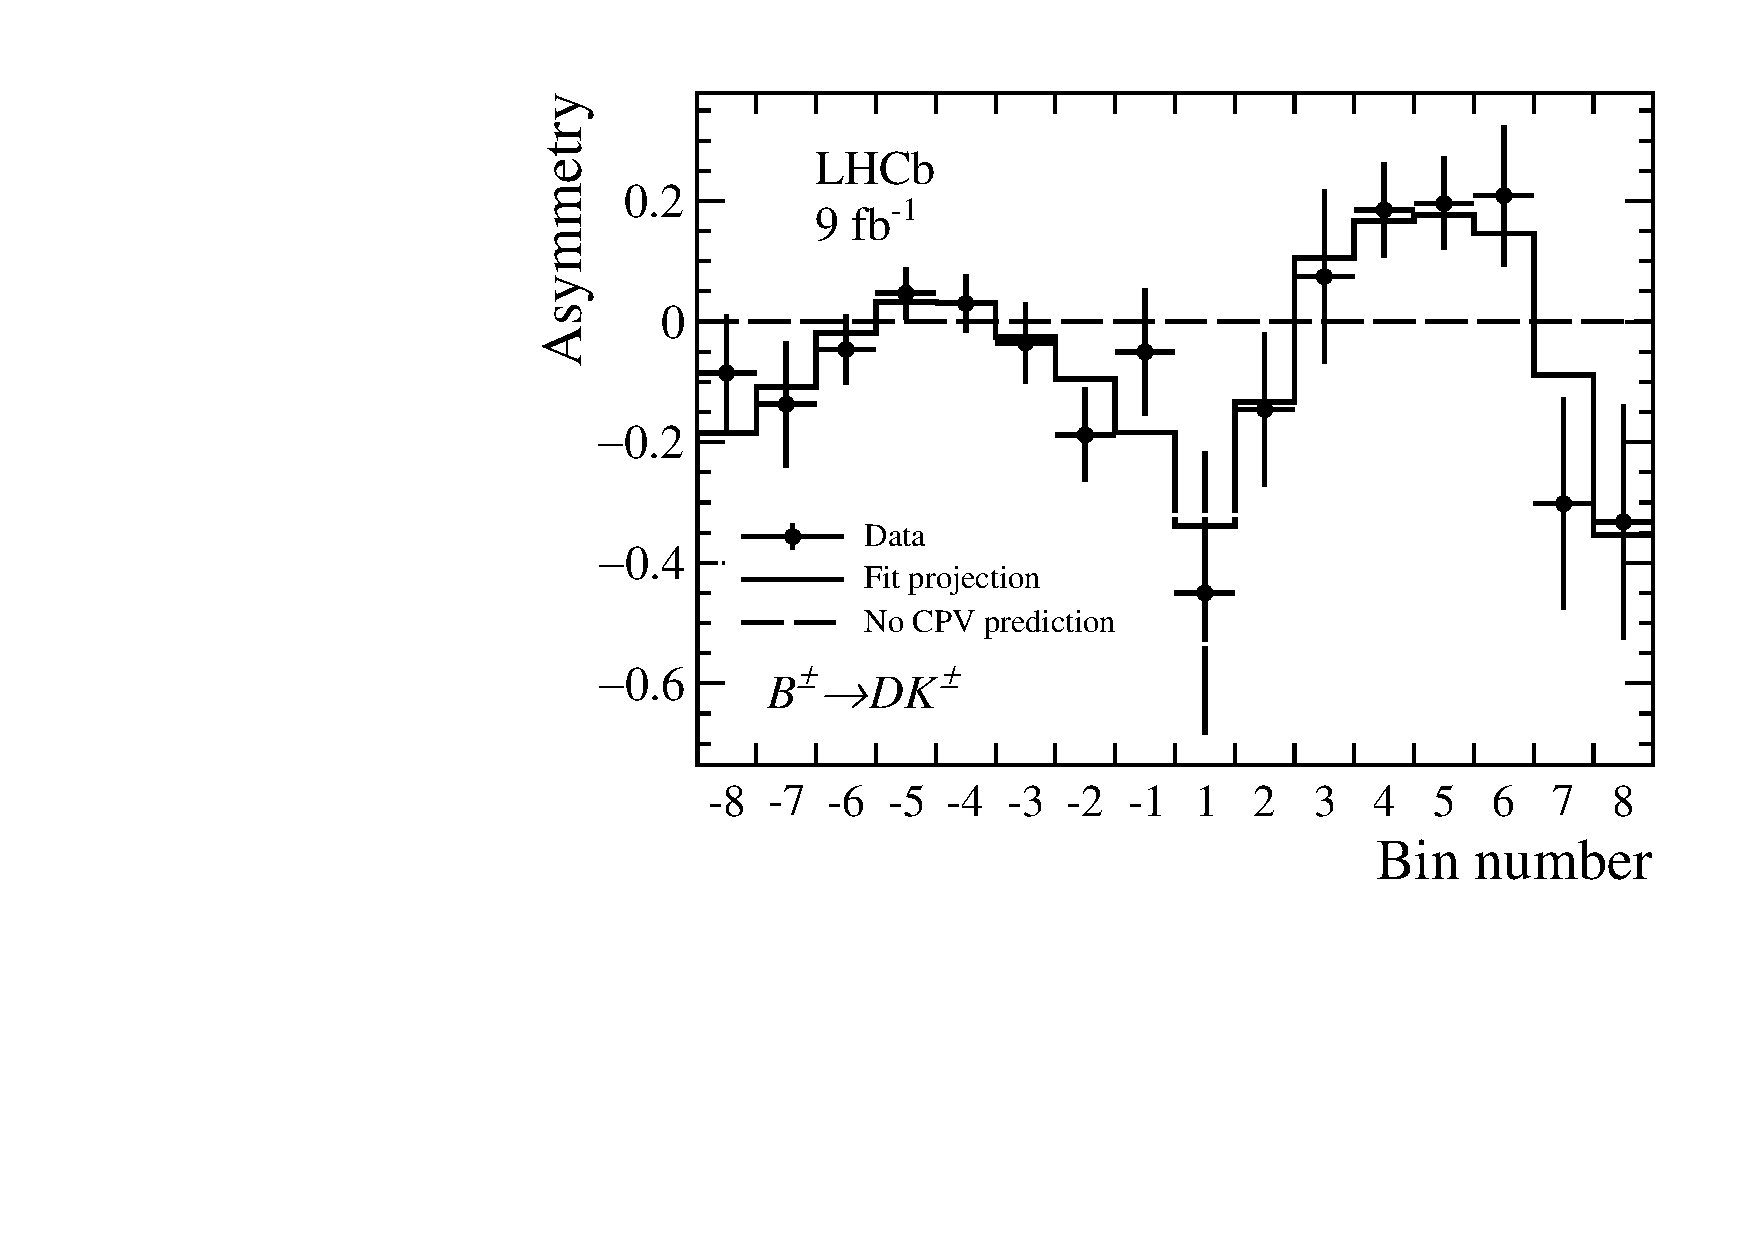
\includegraphics[height = 5cm]{Plots/BinAsymmetries_dk.pdf}
    \vspace{-0.4cm}
    \caption*{\tiny Eur. Phys. J. C \textbf{83}, 547 (2023)}
  \end{figure}
  \vspace{-0.5cm}
  \begin{itemize}
    \setlength\itemsep{0.5em}
    \item{Clear bin asymmetries are seen, and the non-trivial distribution is driven by the change in strong-phase differences across phase space}
    \item{While the interpretation of $\gamma$ require charm inputs, the observed bin asymmetries are model independent}
  \end{itemize}
\end{frame}

\begin{frame}{Phase-space binned $B^\pm\to[K^+K^-\pi^+\pi^-]_DK^\pm$}
  \begin{center}
    \large From the phase-space binned asymmetries, we obtain:
  \end{center}
  \begin{itemize}
    \item{$\gamma = (116^{+12}_{-14})^\circ$}
    \item{$\delta_D^{DK} = (81^{+12}_{-14})^\circ$}
    \item{$r_B^{DK} = 0.110^{+0.020}_{-0.020}$}
  \end{itemize}
  \vspace{-0.2cm}
  \begin{figure}[htb]
    \centering
    \begin{subfigure}{0.5\textwidth}
      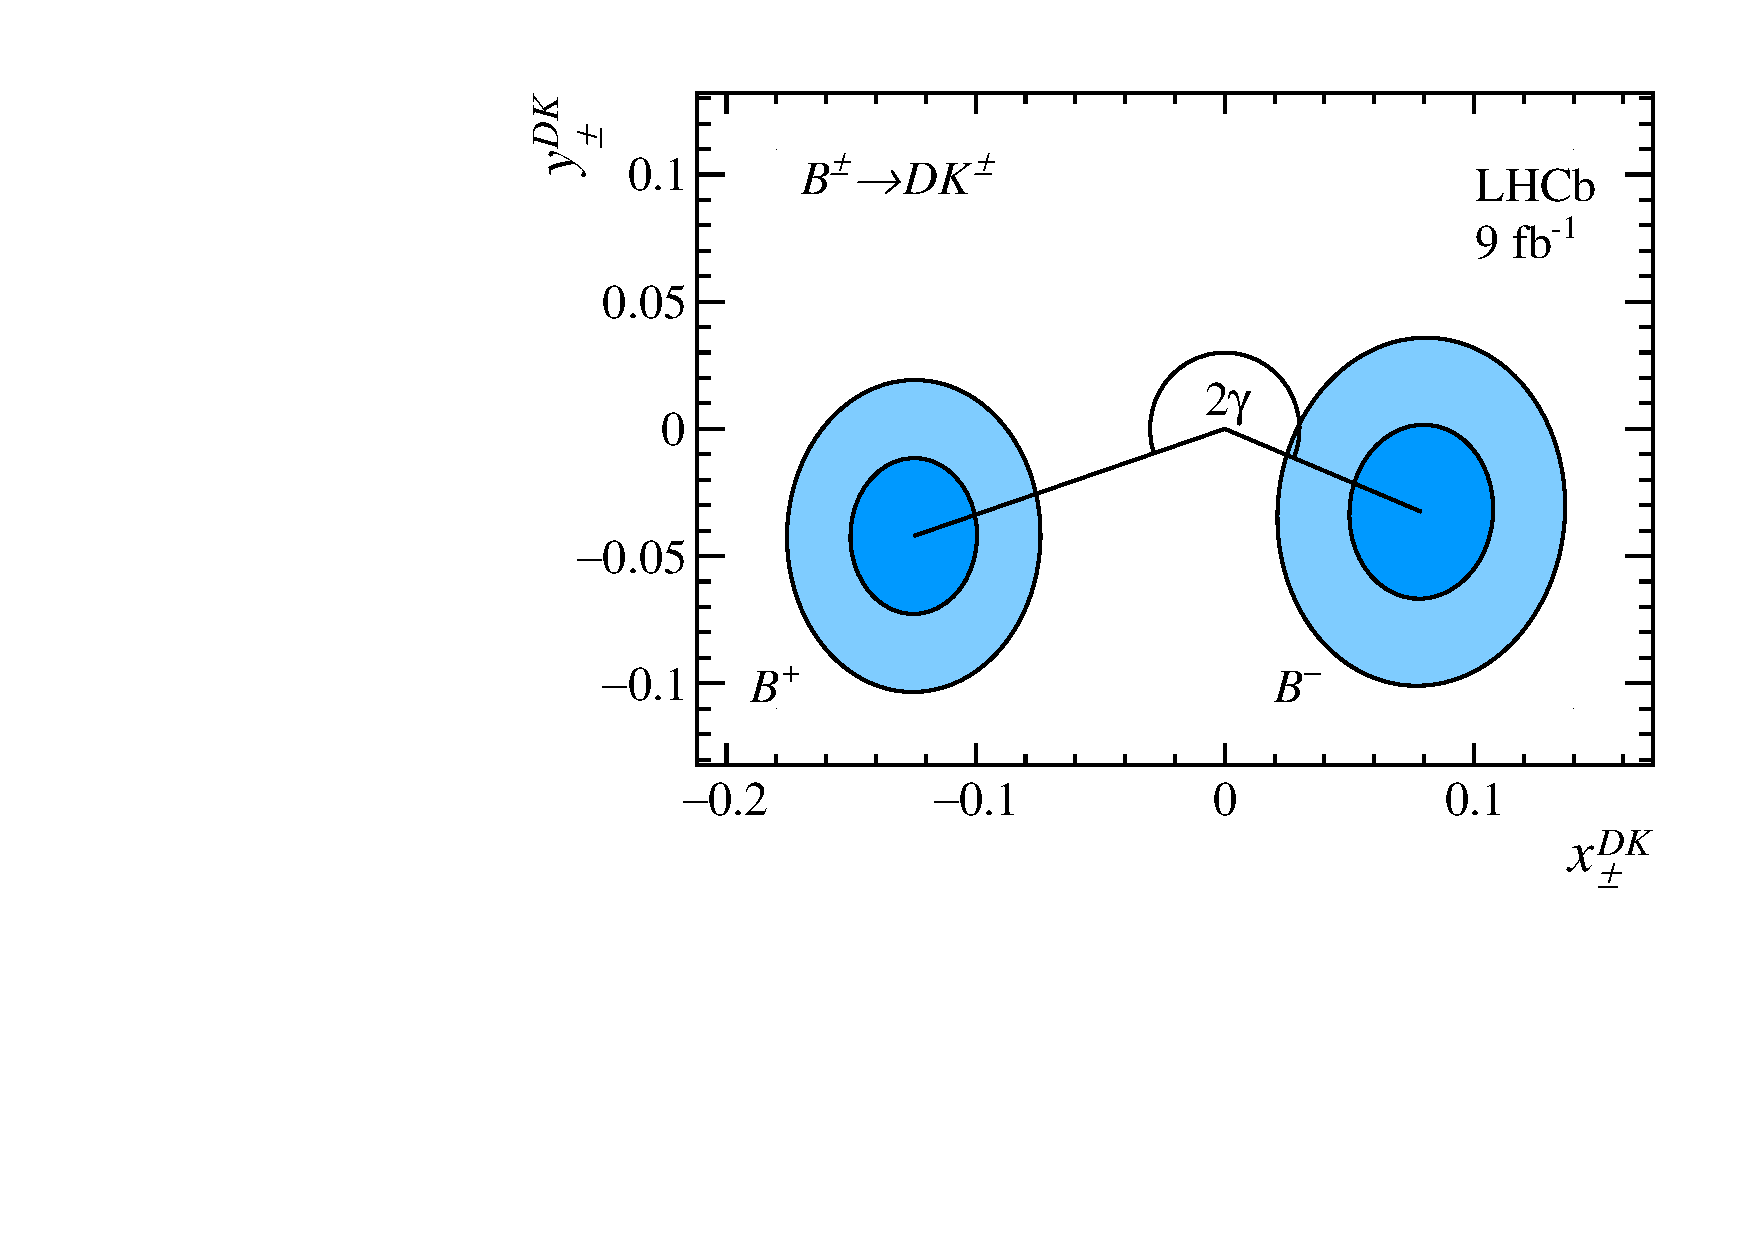
\includegraphics[width=1\textwidth]{Plots/B2DK_CP_Observables_Contours.pdf}
    \end{subfigure}%
    \begin{subfigure}{0.5\textwidth}
      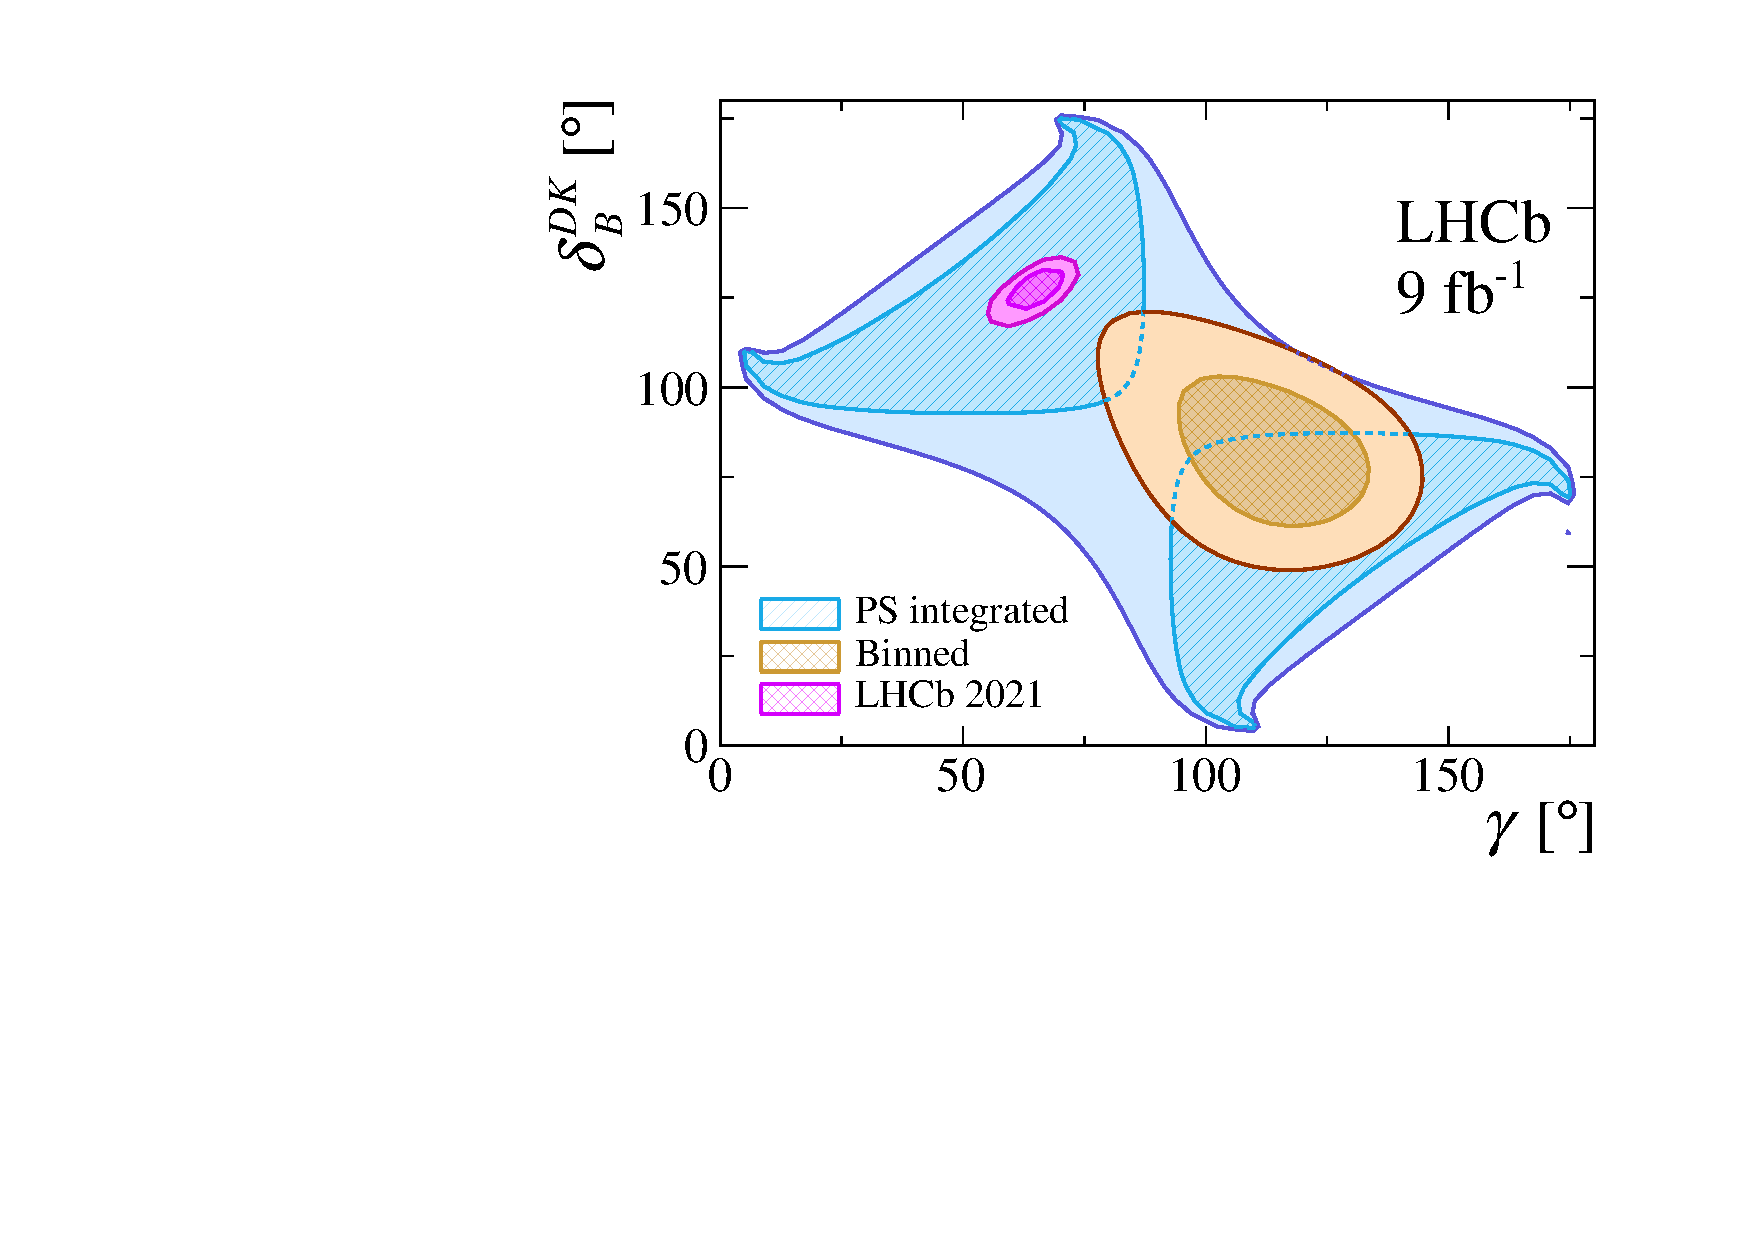
\includegraphics[width=1\textwidth]{Plots/gammacharm_lhcb_KKpipi_GLW_KKpipi_GGSZ_lhcb_2020_beauty_and_charm_g_d_dk.pdf}
    \end{subfigure}
    \vspace{-0.5cm}
    \caption*{\tiny Eur. Phys. J. C \textbf{83}, 547 (2023)}
  \end{figure}
  \vspace{-0.5cm}
  \begin{center}
    {\large These results are \underline{model dependent}, and will be updated once BESIII strong-phase inputs are available}
  \end{center}
\end{frame}

\section{Summary and future prospects}
\begin{frame}{Summary and future prospects}
  \begin{center}
    {\huge The angle $\gamma$ of the Cabibbo-Kobayashi-Maskawa ansatz} \\~\\
    {\large Almost at the end of this seminar, but not the end of the journey!}
  \end{center}
\end{frame}

\begin{frame}{Future prospects}
  \vspace{0.0cm}
  {\Large Future prospects:}
  \vspace{0.3cm}
  \begin{itemize}
    \setlength\itemsep{1.0em}
    \item{The measurements presented today will make valuable improvements to future $\gamma$ combinations}
    \item{Several interesting Run 1$+$2 results are in the pipeline:}
    \begin{enumerate}
      \setlength\itemsep{0.3em}
      \item{Update of $B^\pm\to[K^+K^-\pi^+\pi^-]_Dh^\pm$ with charm inputs from BESIII}
      \item{GLW and ADS results from $B^0\to DK^{*0}$ could shed light on the (slight) tension between $B^0$ and $B^\pm$}
      \item{Time-dependent measurements, such as $B_s^0\to D_s^-K^+$ with Run 2, will be interesting to compare with results from $B^\pm$/$B^0$}
    \end{enumerate}
    \item{LHCb, during Run 3 and 4, anticipates to collect five times more data}
    \begin{itemize}
      \item{$\gamma$ is still dominated by statistical uncertainties!}
    \end{itemize}
  \end{itemize}
\end{frame}

\begin{frame}{Summary and future prospects}
  \vspace{0.0cm}
  {\Large In summary:}
  \vspace{0.3cm}
  \begin{enumerate}
    \setlength\itemsep{1.0em}
    \item{Long journey towards a precise determination of $\gamma$}
    \item{Two recent results of $B^\pm\to D^*h^\pm$ and $B^0\to DK^{*0}$ with $D\to K_S^0h^+h^-$, using external inputs from BESIII}
    \begin{itemize}
      \item{Unique synergy between beauty and charm factories}
    \end{itemize}
    \item{A binned measurement with the channel $B^\pm\to[K^+K^-\pi^+\pi^-]_DK^\pm$ has been performed for the first time}
    \begin{itemize}
      \item{Need external inputs for charm strong-phases from BESIII}
    \end{itemize}
    \item{LHCb is on track to reach a $1^\circ$ precision after Run 3 and 4!}
  \end{enumerate}
  \vspace{0.4cm}
  \begin{center}
    {\huge \phantom{Thanks for your attention!}}
  \end{center}
\end{frame}

\begin{frame}{Summary and future prospects}
  \vspace{0.0cm}
  {\Large In summary:}
  \vspace{0.3cm}
  \begin{enumerate}
    \setlength\itemsep{1.0em}
    \item{Long journey towards a precise determination of $\gamma$}
    \item{Two recent results of $B^\pm\to D^*h^\pm$ and $B^0\to DK^{*0}$ with $D\to K_S^0h^+h^-$, using external inputs from BESIII}
    \begin{itemize}
      \item{Unique synergy between beauty and charm factories}
    \end{itemize}
    \item{A binned measurement with the channel $B^\pm\to[K^+K^-\pi^+\pi^-]_DK^\pm$ has been performed for the first time}
    \begin{itemize}
      \item{Need external inputs for charm strong-phases from BESIII}
    \end{itemize}
    \item{LHCb is on track to reach a $1^\circ$ precision on $\gamma$ after Run 3 and 4!}
  \end{enumerate}
  \vspace{0.4cm}
  \begin{center}
    {\huge Thanks for your attention!}
  \end{center}
\end{frame}

\end{document}
